\documentclass[acmsmall,screen,review,nonacm]{acmart}

% --- Journal metadata (volume, number, article and DOI are set by ACM) ----
\acmJournal{TOCT}

% --- Packages ---------------------------------------------------------------
% acmart already loads amsmath, amsthm (acmthm=true), natbib, hyperref,
% graphicx, xcolor and booktabs.
\usepackage{mathtools}
\usepackage{array}
\usepackage[nameinlink,noabbrev]{cleveref}

\AtEndPreamble{%
  \theoremstyle{acmdefinition}%
  \newtheorem{remark}[theorem]{Remark}%
  \theoremstyle{acmplain}}

\newcommand{\wt}{\operatorname{wt}}
%                 A comment "% gloss: <term or G-id>" on the same or an
%                 adjacent line marks a gloss given in other words.
% % lint: lean-table begin / end
%                 brackets the Appendix A correspondence table, the only
%                 place where Lean identifiers may appear.
% % lint: program begin / end
%                 brackets the origin paragraph (Section 1.5) and the marked
%                 reading paragraph (Section 8.2), the only places where the
%                 program vocabulary may appear.
\newcommand{\defterm}[1]{\emph{#1}}
% Release identity (DOI, version, date) written by the Zenodo toolkit's
% paper_set_release.py.
% Generated by scripts/paper_set_release.py.
% The date is the UTC date when this submission was assembled.
\newif\ifpaperhasdoi
\paperhasdoitrue
\newcommand{\paperdoi}{10.5281/zenodo.24494014}
\newcommand{\manuscriptversion}{Preprint v1.0}
\newcommand{\manuscriptdate}{25 November 2026}
\newcommand{\manuscriptyear}{2026}

% Zenodo archive DOI (reserved 2026-11-24, deposition 24494014; see
% paper/submission/zenodo-release.json).
\newcommand{\archivedoi}{10.5281/zenodo.24494014}
% Shared notation (moved from Section 3)
\newcommand{\NN}{\mathbb{N}}
\newcommand{\QQ}{\mathbb{Q}}
\newcommand{\RR}{\mathbb{R}}
\newcommand{\supp}{\operatorname{supp}}
\newcommand{\sgn}{\operatorname{sgn}}
\newcommand{\core}{\operatorname{core}}
\newcommand{\SC}{\operatorname{sc}}
\newcommand{\FQ}{\mathcal F_{\QQ}}
\newcommand{\FR}{\mathcal F_{\RR}}

% --- Front matter ---------------------------------------------------------------
\title[One Word Against Two]{One Word Against Two: The Complexity of Revising Markov Laws Under Held Tests}

\author{Ioannis Tsiokos}
\orcid{0009-0009-7659-5964}
\affiliation{%
  \institution{Automorph Inc.}
  \city{Athens}
  \country{Greece}}
\email{ioannis@automorph.io}
\renewcommand{\shortauthors}{Ioannis Tsiokos}

\begin{abstract}
We prove that, for explicitly presented labeled shared-probe Markov chains with a hidden register, revising parameters under held tests goes from P-complete to PSPACE-hard at one step of test syntax. A word test equates joint probabilities of two sets of words with each final observed base state, from every initial full state. Its words share one positive length within the model's bound. Value tests fix a probe eigenvalue or an equal-length word-probability ratio. At a fixed profile (labeled transition support, register partitions, held tests), fine reachability asks for a finite feasible rational chain between supplied endpoints at every $\varepsilon>0$, each step changing every full-state labeled transition probability by less than $\varepsilon$. On promised-feasible inputs this is P-complete under log-space reductions if every word test compares single words, with polynomial-size certificates for both answers. It is PSPACE-hard if exactly one compares a word with a sum of two distinct words, the others single words, even at a supplied inverse-polynomial tolerance. Single-word tests give binomial probe equations that become vacuous when both monomials vanish. Peeling damps coordinates to zero along monomial curves with nonnegative integer weights that preserve the active equations, then recomputes them. At a fixed single-word profile each signed support has a unique terminal signed support, its signed core, and feasible endpoints are finely reachable exactly when their cores agree. In the reduction from nondeterministic constraint logic, a positive sum keeps at least one summand nonzero; further equations and budgets make the represented orientations legal. For budgeted signed-binomial systems with promised bounded rational solution sets and supplied feasible rational endpoints, fine connectivity by sup-norm steps is P-complete; growing numbers of affine trinomials make it PSPACE-hard.
\end{abstract}

% CCS 2012 concepts (concept IDs as used in published ACM CCS markup).
\begin{CCSXML}
<ccs2012>
   <concept>
       <concept_id>10003752.10003777.10003779</concept_id>
       <concept_desc>Theory of computation~Problems, reductions and completeness</concept_desc>
       <concept_significance>500</concept_significance>
   </concept>
   <concept>
       <concept_id>10003752.10003777.10003783</concept_id>
       <concept_desc>Theory of computation~Algebraic complexity theory</concept_desc>
       <concept_significance>300</concept_significance>
   </concept>
</ccs2012>
\end{CCSXML}

\ccsdesc[500]{Theory of computation~Problems, reductions and completeness}
\ccsdesc[300]{Theory of computation~Algebraic complexity theory}

% Keywords: the candidates of the target profile, in American spelling.
\keywords{reconfiguration, P-completeness, PSPACE-hardness, labeled Markov chains, binomial systems, exact rational arithmetic, formal verification}

\begin{document}

\maketitle

\noindent{\small \manuscriptversion, \manuscriptdate. \copyright~\manuscriptyear{} Automorph Inc. CC-BY 4.0. Zenodo DOI: \href{https://doi.org/\paperdoi}{\paperdoi}.}


\section{Introduction}\label{sec:intro}

\paragraph{What is new.}
% gloss: labeled Markov chain
% gloss: feasible
% gloss: held test
% gloss: word test
% gloss: P-complete
% gloss: PSPACE-hard
% gloss: fine reachability
\begin{itemize}
\item \emph{A sharp complexity boundary} (Theorem~\ref{thm:boundary}).
% gloss: configuration (defined in Section 1.1, as the block's last sentence says)
% gloss: profile
% gloss: at a fixed profile
% gloss: word test
For labeled Markov chains with held tests: can two feasible configurations
at a fixed profile be joined by arbitrarily small feasible rational steps?
% gloss: P-complete
% gloss: PSPACE-hard
This is P-complete when every word test compares single words, and
PSPACE-hard when exactly one compares a word with the sum over two distinct
words and the rest compare single words.
% gloss: signed core
\item \emph{The signed core} (Theorems~\ref{thm:core}
and~\ref{thm:fixed-profile}), a combinatorial invariant that decides the
tractable side, with short certificates for both answers.
% gloss: budgeted signed-binomial system
\item \emph{A model-free version} (Corollary~\ref{cor:intro-algebraic}).
For budgeted signed binomials with a promised bounded rational solution
set, rational fine connectivity is P-complete. Allowing a growing number
of equations $x_j+y_j=1$ makes it PSPACE-hard.
% gloss: acquisition timing
\item \emph{Timing matters} (Theorem~\ref{thm:acquisition}). Adding a test
early can block revisions that adding it late allows.
\end{itemize}
Section~\ref{sec:question} defines the terms, and
Theorem~\ref{thm:intro-boundary} and Table~\ref{tab:results} give the
precise statements.


\subsection{The question}\label{sec:question}

Reconfiguration problems ask whether one feasible solution of a
constraint system can be turned into another by small steps that each
stay feasible~\cite{gopalan,hearndemaine,ito}.
% gloss: feasible
We ask this question for rational parameters in a family of Markov chains whose
transitions carry labels~\cite[Definition~1]{chenkiefer2014}.
% gloss: labeled Markov chain
A \defterm{word test} compares \defterm{words}, strings of transition
labels, all of the same positive length within the model's length bound.
In a word-against-word test, the joint probability of the first word
and each final observed base state must equal that of the second word,
from every initial state of the chain.
In a \defterm{word-against-pair} test, the single word's joint probability
must equal the sum of the corresponding joint probabilities for two distinct
words. Given two feasible rational parameter vectors at a common profile
(defined below),
% gloss: profile
can one be revised into the other, for every $\varepsilon>0$, by a finite
sequence of feasible rational parameter vectors at that profile? Each step
must change every full-state labeled transition probability by less
than~$\varepsilon$.

The chain is built so that word tests yield simple equations. A
\defterm{full state} $(g,r)$ pairs an observed base state~$g$ with a hidden
\defterm{register} value~$r$. Each label~$m$ moves base states by a
kernel~$Q_m$, and all these kernels share a fixed family of $\pm1$-valued
\defterm{probes} on the base states as eigenvectors. The \defterm{eigenvalue}
$\alpha_{mi}$ of $Q_m$ on probe~$i$ is the label's \defterm{signed bias}:
from any full state, conditional on label~$m$, probe~$i$ keeps its sign with
probability $(1+\alpha_{mi})/2$, and an eigenvalue of zero makes the new sign
fair. On each probe, a word's eigenvalue is the product of its labels'
eigenvalues. A word-against-word test therefore gives binomial equations: one
equating word probabilities, and one \defterm{probe equation} per probe
equating eigenvalue products.

The \defterm{Markov law} of the title is the parameter vector: label
probabilities, eigenvalues, and register tables. A \defterm{configuration}
pairs a parameter vector with its \defterm{profile}: positive labeled
transitions, register groupings at each level (Section~\ref{sec:problem}),
and \defterm{held} tests.
% gloss: held test
We keep this profile fixed; every configuration in the sequence must satisfy
all tests held at its profile.

\begin{figure}[t]
  \centering
  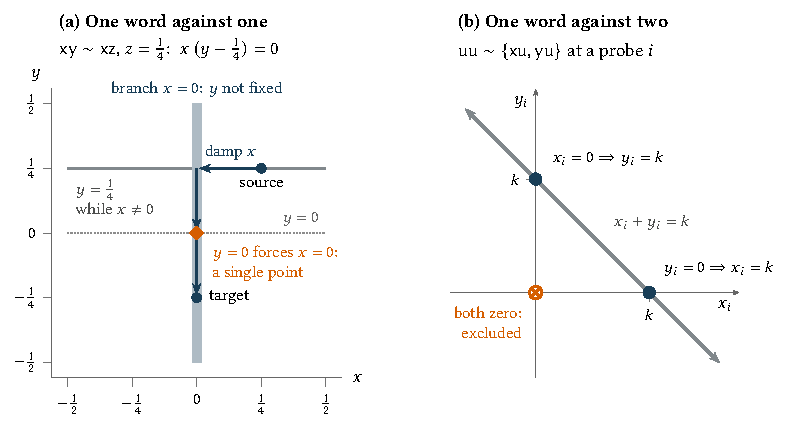
\includegraphics{figures/fig1-mechanism.pdf}
  \Description{Two panels. Panel (a), titled one word against one, plots y against x for the equation x(y - 1/4) = 0 with z = 1/4. A horizontal line at y = 1/4 holds while x is nonzero. On the shaded branch at x = 0, the equation no longer fixes y, and the branch extends from y = -1/2 to y = 1/2. A horizontal arrow damps x from the source (1/4, 1/4) to (0, 1/4). Two downward arrows lead through (0, 0) to the target (0, -1/4). A marked point at the origin notes that setting y = 0 instead forces x = 0, a single point. Panel (b), titled one word against two, shows the load line x_i + y_i = k in the (x_i, y_i) plane at a probe i. Its intercepts at (0, k) and (k, 0) are marked: if one summand is zero the other equals k. The origin is crossed out because both summands cannot vanish.}
  \caption{How the two test syntaxes differ; here $x,y,z$ and $x_i,y_i$ are label eigenvalues on shared $\pm1$ probes (Section~\ref{sec:question}).
% gloss: peeling step (the staged example, next paragraph; the float is placed early for layout)
% gloss: value test (a held value test that fixes one eigenvalue: a calibration)
(a) In the staged example, a held value test fixes (calibrates) $z=1/4$, and the word-against-word test $\mathsf{xy}\sim\mathsf{xz}$ gives $xy=xz$. While $x\neq0$ this fixes $y=1/4$. A \emph{peeling step} damps $x$ to~$0$. On $x=0$ both monomials vanish, so the test still passes while $xy=xz$ stops constraining $y$, letting $y$ move through rationals to $-1/4$. Setting $y=0$ instead forces $x=0$, a single point. (b) In the hard construction of Section~\ref{sec:hard} (with different labels),
% gloss: load label (the calibrated label whose word is compared with the pair; Section 5.1)
one word-against-pair test, with forced label probabilities and a fixed (calibrated) load label, gives the load equation $x_i+y_i=k>0$ at each probe~$i$. If one summand is zero, the other equals~$k$; both cannot vanish. The remaining constraints (Figure~\ref{fig:ncl}) decide which points on this line and which moves are feasible, and at a given feasible configuration an edge may allow only one orientation. In both panels only eigenvalues vanish; the set of positive labeled transitions does not change.}\label{fig:mechanism}
\end{figure}

Two small examples, each with two base states and one probe, show what is at
stake: the \defterm{staged example} (displayed labels $\mathsf x,\mathsf y,\mathsf z$;
Figure~\ref{fig:mechanism}(a)) and the \defterm{sign example} (labels
$\mathsf y,\mathsf z$). Throughout, each italic letter $x,y,z$ denotes the
eigenvalue of the matching roman label. In both examples, a held
\defterm{calibration} fixes $z=1/4$. In the staged example, the held word
test $\mathsf{xy}\sim\mathsf{xz}$ gives $xy=xz$, fixing $y=1/4$ while
$x\neq0$. A \defterm{peeling step} multiplies each eigenvalue by $t^{\eta}$,
with its own nonnegative integer weight~$\eta$, as $t$ falls from $1$ to~$0$.
The weights must preserve every binomial equation \defterm{active} on the
starting support. An equation is active there exactly when neither monomial
is forced to vanish by zeros outside that support. Here
$\eta_x=1$ and $\eta_y=\eta_z=0$, sending $x$ to~$0$. The word test still
passes, its probe equation becomes inactive, and $y$ then moves to $-1/4$ in
arbitrarily fine rational steps.

The sign example has a one-value register and a probability floor of $1/2$, a
lower bound on each label's probability;
% gloss: probability floor
since the two label probabilities sum to~$1$, both equal $1/2$. With the
calibration $z=1/4$ and $\mathsf{yy}\sim\mathsf{zz}$ held, the only feasible
values of $y$ are $1/4$ and $-1/4$. Switching signs changes each labeled
transition-table entry for $\mathsf y$ by $1/8$ in absolute value and fixes
the $\mathsf z$ entries, so a feasible sequence joins them exactly when
$\varepsilon>1/8$. Passing the same tests does not settle reachability. We
ask how hard it is to decide \defterm{fine reachability}, the existence of a
feasible connecting sequence at every positive tolerance. We also ask how the
complexity changes when exactly one word test is word-against-pair and all
other word tests compare single words (Figure~\ref{fig:mechanism}(b)).


\subsection{Our results}\label{sec:results-intro}

Our main theorem gives a tractable--hard boundary for reconfiguration of
exact rational parameter spaces. The two-way classification of Gopalan
et al.~\cite{gopalan}, with Schwerdtfeger's
correction~\cite{schwerdtfeger}, and the three-way classification of Kimura and
Suzuki~\cite{kimurasuzuki} are analogies for this change in complexity at
one step of test syntax.
The title's \defterm{one word against two} names the two test syntaxes:
every word test compares one word with one (the \emph{single-word class}),
or exactly one compares a word with two distinct words and the rest compare
single words.
% gloss: value test
Value tests, which fix an eigenvalue or a probability ratio, are allowed in
both classes. The word-against-pair test imposes $1+|I|$ equations
(Section~\ref{sec:problem}), possibly dependent: one mass equation on word
probabilities and one per probe in the probe set~$I$.
Theorem~\ref{thm:intro-boundary} concerns the shared-probe family of
Section~\ref{sec:model}: labeled Markov chains whose labels act by eigenvalues
on shared probes, with a hidden register. Keeping the profile fixed ensures
that hardness does not come from profile changes.

\begin{theorem}[Informal; see Theorem~\ref{thm:boundary}]\label{thm:intro-boundary}
For explicitly presented shared-probe models encoded in binary, given two
rational configurations $A,B$ promised feasible at a fixed profile:
\begin{enumerate}
% gloss: P-complete
\item[(i)] If every word test compares one word with one, fine reachability
is P-complete under deterministic log-space many-one reductions, with
polynomial-size, polynomial-time-checkable certificates for both answers.
\item[(ii)] If exactly one word test compares a single word with the sum over
two distinct words and all others compare single words, fine reachability is
PSPACE-hard under polynomial-time many-one reductions. The same reduction
proves PSPACE-hardness of sequence existence at a supplied positive rational
tolerance whose reciprocal is polynomially bounded in the length of the
reduction's input.
\end{enumerate}
\end{theorem}

% gloss: signed core
% gloss: G9
% gloss: finely reachable (Section 1.1, fine reachability)
% gloss: reversal (Section 2.1)
\paragraph{Part (i) in words.} In the single-word class, $B$ is finely
reachable from $A$ exactly when both have the same signed core under the
profile's eigenvalue constraints, including the fixed reversal equations
(Theorem~\ref{thm:fixed-profile}; omitting reversal equations can change the
verdict).
The signed core records only the eigenvalue coordinate indices surviving
iterated peeling and their signs, not their magnitudes.
Certificates record peeling stages and a terminal Gordan certificate for each
endpoint, containing no connecting sequence. %
There are algebraic instances for which every feasible connecting sequence
at tolerance $1/4$ contains a coordinate value whose reduced denominator has
exponentially many binary digits in the number of coordinates
(Proposition~\ref{prop:long-sequences}).

\paragraph{Part (ii) in words.} The reduction is from nondeterministic
constraint logic (NCL)~\cite{hearndemaine}. Each edge becomes a probe whose
nonzero summands in the load equation $x_i+y_i=k>0$
(Figure~\ref{fig:mechanism}(b)) give its candidate orientations. A zero
summand forces the other to equal~$k$, though both may be nonzero in between.

% gloss: cover
% gloss: profile step
% gloss: attained (Section 2.3)
\paragraph{The strengthening.} Theorem~\ref{thm:directed} also allows
profile steps to a covering attained profile (adding tests, shrinking
support, or refining register partitions; Section~\ref{sec:directed}) while
keeping label probabilities and eigenvalues, and register tables when support
is unchanged. In the single-word class, fine reachability holds exactly when
the target profile is at or above the source profile and both signed cores
agree under the source profile's constraints.

\paragraph{Scope.} Both lower bounds hold with every test held throughout
and a one-value hidden register; Theorem~\ref{thm:boundary} lists the
remaining restrictions.
% gloss: exactly one word-against-pair test
% gloss: G5
``Exactly one'' counts word-against-pair tests in the model's word-test list;
other word tests and calibrations are unlimited. We prove no upper bound for
part~(ii); one in PSPACE would put rational-zero existence for integer
polynomials in PSPACE (Theorem~\ref{thm:rational-roots}).

\begin{corollary}[The model-free form, informal; see Corollaries~\ref{cor:algebraic} and~\ref{cor:real-complexity}]\label{cor:intro-algebraic}
For an explicit binary budgeted signed-binomial system (equations
$x^a=c\,x^b$ with $a,b\in\NN^J$ and $c\in\QQ$ on coordinates allowed to be
zero or negative, with $\ell^1$ budgets)
% gloss: ℓ¹ budget κ (absolute-value budgets; Section 2.1)
and two supplied feasible rational points:
\begin{enumerate}
\item[(i)] Under the promise that the feasible rational set is bounded,
\defterm{fine connectivity} (joining them at every rational $\varepsilon>0$
by feasible rational steps changing each coordinate by less than~$\varepsilon$)
is P-complete under deterministic log-space many-one reductions meeting the
promise.
% gloss: affine trinomial
\item[(ii)] Allowing a growing number of scalar affine trinomials
$x_j+y_j=k$ (even with $k=1$ throughout) makes fine connectivity PSPACE-hard
under polynomial-time many-one reductions meeting the same promise, with no
upper bound proved here.
\item[(iii)] In the full real locus, membership of two feasible rational
points in one real path component is P-complete for budgeted binomial
systems, and PSPACE-complete with a growing number of equations $x_j+y_j=1$
(Corollary~\ref{cor:real-complexity}); neither upper bound requires
boundedness.
\end{enumerate}
\end{corollary}

\paragraph{Reading the corollary.} The split already occurs for explicit
algebraic systems, with no Markov model. The tractable side contrasts with
real two-point connectivity, which is PSPACE-hard already for noncrossing
planar tree-linkage configuration spaces~\cite[Theorem~2]{altknauerrotewhitesides}.
Following Canny~\cite{canny93}, Basu, Pollack and Roy give a singly
exponential roadmap algorithm for explicit real semialgebraic sets with
algebraically encoded endpoints~\cite[Theorem~3]{basupollackroy}.
The direct algebraic reduction uses $|E|$ normalized affine trinomials
(Section~\ref{sec:real-ncl}), leaving PSPACE-hardness with one scalar affine
trinomial open.

\begin{table}[tp]
\caption{Results at a glance. Decision inputs are explicitly encoded in
binary, with supplied feasible rational endpoints. P-completeness is under
deterministic log-space many-one reductions, and PSPACE lower bounds are
under polynomial-time many-one reductions. Source~$A$, target~$B$; $\preceq$
is the profile order (Section~\ref{sec:directed}); $A^+$ is $A$ after an
acquisition.}\label{tab:results}
\footnotesize\setlength{\tabcolsep}{4pt}\renewcommand{\arraystretch}{0.88}
\begin{tabular}{@{}>{\raggedright\arraybackslash}p{0.25\linewidth}p{0.60\linewidth}p{0.11\linewidth}@{}}
\toprule
Problem & Result & Where\\
\midrule
\multicolumn{3}{@{}l}{\emph{Main results}}\\[2pt]
Single-word class, fixed profile & P-complete, with polynomial-size,
polynomial-time-checkable certificates for both answers; decided by equal
signed cores under the common profile's constraints. &
Thms~\ref{thm:boundary}(i), \ref{thm:fixed-profile}\\
% gloss: G9
Single-word class, with profile steps & P-complete, with the same certificate
guarantees; holds exactly when $p_A\preceq p_B$ and signed cores agree under
the source profile's constraints. & Thm~\ref{thm:directed}\\
% gloss: G5
% gloss: G7
Exactly one word-against-pair test & Fixed profile: PSPACE-hard for fine
reachability and at a supplied tolerance (verdict agrees at that tolerance
and below on NCL outputs); rational-zero existence reduces to it; no upper
bound proved. & Thms~\ref{thm:boundary}(ii), \ref{thm:rational-roots}\\
Budgeted binomials: fine connectivity (bounded rational set) & P-complete. &
Cor.~\ref{cor:algebraic}\\
\quad plus growing affine trinomials $x_j+y_j=k$ (same promise) &
PSPACE-hard; no upper bound proved. & Cor.~\ref{cor:algebraic}\\
Budgeted binomials: real path-component membership & Full real locus, two
supplied feasible rational endpoints: P-complete for budgeted binomials, and
PSPACE-complete with growing equations $x_j+y_j=1$; upper bounds need no
boundedness, and hardness already holds on bounded real loci. &
Cor.~\ref{cor:real-complexity}\\[3pt]
\multicolumn{3}{@{}l}{\emph{Further results}}\\[2pt]
Single-word class, no nonzero calibration held at source & Fine reachability
holds exactly when $p_A\preceq p_B$. & Thm~\ref{thm:no-calibration}\\
% gloss: undecidable
% gloss: G14
One word-against-pair test, fixed counts & For each fixed $N$, quartic
rational solvability reduces to fine reachability and sequence existence at
one fixed positive tolerance. Probe and label counts depend only on~$N$.
Undecidability is conditional on the Bhargava--Burungale quartic
theorem~\cite[Corollary~1.2(3)]{bhargavaburungale}. & Cor.~\ref{cor:quartic}\\
One word-against-pair test, zero probes & If the test is unheld at the
source, the directed profile order decides fine reachability. If held, two
subcases are polynomial-time. The remaining subcase has an exact
rational-ratio closure criterion whose decidability is open. & Props.~\ref{prop:zero-probes},
\ref{prop:zero-probe-closure}\\
Real versus rational, one word-against-pair test & Examples with zero probes
(and a held probability-ratio test) and with one probe have a real path but
fail fine rational reachability. & Props.~\ref{prop:one-probe},
\ref{prop:zero-probe-fermat}\\
One-state subclass & Length-two tests with growing word-against-pair tests:
PSPACE-hard at a fixed profile and at the supplied tolerance; rational-zero
existence also reduces to it. & Prop.~\ref{prop:one-state}\\
Acquisition timing (test acquired before or after revision) & Early
acquisition can block fine reachability that late acquisition allows, even when
both endpoints pass the new test. For the feasible acquisition keeping the
parameter vector fixed, with $p_A\preceq p_{A^+}\preceq p_B$, two signed-core
checks decide timing in polynomial time (single-word class). With both
word-test shapes, the criterion compares components in the projected rational
closures $\mathcal K_{p_A}$ and $\mathcal K_{p_{A^+}}$ (no general algorithm
given). & Thms~\ref{thm:acquisition}, \ref{thm:projected-components}\\
% gloss: real component
% gloss: G22
Budgeted binomials: real components (no boundedness assumed) & Connected and
path components are classified by the signed core. & Cor.~\ref{cor:real}\\
Separation cutoff for distinct signed cores (bounded rational locus) & Sup
distance $\ge 2^{-D}$, with $\log D$ polynomially bounded in binary system
length excluding endpoints; transfers to the Markov metric. Expanded rational
cutoff denominators can need exponentially many digits. Doubly exponential
scale and repeated-squaring witness via Jeronimo, Perrucci and
Tsigaridas~\cite{jeronimoperruccitsigaridas}. & Prop.~\ref{prop:separation}\\
\bottomrule
\end{tabular}
\end{table}

\paragraph{Contributions.}
\begin{enumerate}
\item \emph{The boundary} (Theorem~\ref{thm:intro-boundary},
Table~\ref{tab:results}). At a fixed profile on promised-feasible rational
inputs, fine reachability is P-complete with polynomial-size certificates for
% gloss: polynomial-size certificates (no connecting sequence; Part (i) in words)
both answers in the single-word class, and PSPACE-hard with exactly one
word-against-pair test.
% gloss: G25
Since the reductions land inside the promise, the single-word problem is in
log-space-uniform NC only if P equals log-space-uniform NC.
To our knowledge, this PSPACE lower bound for fine rational reachability with
exactly one word-against-pair test in this model has not appeared in the
literature. For continuous Petri nets, Fraca and Haddad's Algorithm~2 and
Propositions~27 and~32~\cite{fracahaddad} give the precedents for the
iterated linear-programming upper bound of part~(i) and its lower bound from
monotone circuit value~\cite{goldschlager,greenlawhooverruzzo}.
Here the signed core gives certificates for both answers, and the circuit
reduction uses endpoints sharing a profile and differing in one sign.
\item \emph{The model-free form} (Corollary~\ref{cor:intro-algebraic}). Over
$\RR$, the signed core classifies the components of budgeted signed-binomial
systems without assuming boundedness. For feasible rational endpoints, real
path connectivity agrees with rational fine connectivity when the rational
feasible set is bounded (Corollary~\ref{cor:real}). Real path-component
membership is P-complete, and PSPACE-complete with a growing number of
equations $x_j+y_j=1$ (Corollary~\ref{cor:real-complexity}). The PSPACE
upper bound uses the component algorithm of Heintz, Roy and
Solern\'o~\cite{heintzroysolerno1994components}. We have
not found the rational PSPACE lower bound of
Corollary~\ref{cor:intro-algebraic}(ii) in the literature.
\item \emph{The engine} (Theorems~\ref{thm:core}, \ref{thm:fixed-profile},
\ref{thm:directed} and~\ref{thm:no-calibration}). We have not found
the signed-core classification of Theorem~\ref{thm:core} for bounded
rational feasible sets of budgeted signed-binomial systems stated in the
literature. Newman~\cite{newman}
supplies the confluence antecedent, Tevelev~\cite{tevelev} a chart-limit
antecedent, and \emph{Toric Cubes}~\cite{toriccubes} related fixed-support
geometry. Geiger--Meek--Sturmfels~\cite{geigermeeksturmfels} and
Rauh--Kahle--Ay~\cite{rauhkahleay} give facial-support criteria for positive
model families, while Payne~\cite{payne} and
Soprunova--Sottile~\cite{soprunovasottile} study real toric varieties.
Diaconis--Eisenbud--Sturmfels~\cite{diaconiseisenbudsturmfels} and
Kahle--Rauh--Sullivant~\cite{kahlerauhsullivant} relate discrete
connectivity to binomial ideals for fixed move sets. Our additional steps are
restriction across recomputed supports, the least support, and exact rational
realization under budgets.
\item \emph{Acquisition timing} (Theorems~\ref{thm:acquisition}
and~\ref{thm:projected-components}). Barrett and
Weld~\cite[Sections~3.2--3.3]{barrettweld} study which subgoals can be
achieved and protected in order. Hauser and Latombe analyze component
obstructions at mode intersections~\cite{hauserlatombe}, and Hu, Iyer and
Christensen connect within-manifold roadmaps at
intersections~\cite{huiyerchristensen}. We have not found this
before-and-after criterion for projected rational closures in this model in
the literature.
% gloss: undecidable
% gloss: G14
\item \emph{Exactness} (Corollary~\ref{cor:quartic},
Section~\ref{sec:exactness}). Table~\ref{tab:results} lists the fixed-count
quartic reduction, the real-versus-rational separations, and the zero-probe
cases. That reduction gives undecidability of both target decision problems
for some fixed counts if the Bhargava--Burungale quartic
theorem~\cite[Corollary~1.2(3)]{bhargavaburungale} holds.
\end{enumerate}

\subsection{Techniques}\label{sec:techniques}

The tractable side has one delicate point: tests become inactive as
coordinates vanish. In the staged example, the branch $x=0$ joins opposite
signs of~$y$, so active tests must be recomputed after each peeling step.
Keeping the initial weight balances instead rejects that example
(Figure~\ref{fig:peeling}). Under a fixed test list, permitted peeling steps
restrict to smaller supports, so from a given signed support every terminal
peeling sequence gives the same signed core (Lemma~\ref{lem:restriction}).
After peeling, exact rational interpolation under tight budgets joins points
with the same signed support (Lemma~\ref{lem:interpolation}); in the
P-hardness reduction the surviving signed core computes the circuit.

On the hard side, a positive-sum test keeps constraining when a summand
vanishes: in the load equation $x_i+y_i=k>0$ (Lemma~\ref{lem:engine}) a zero
summand forces the other to carry the load.
A nonzero summand makes the corresponding edge orientation available, and
further tests and budgets encode legality of every represented orientation.
We do not claim that these extra tests and budgets are needed for hardness.
Transfer must hold in both directions and for every feasible step below the
supplied cutoff, including multi-coordinate steps (Section~\ref{sec:transfer}).
The cited hardness results concern different solution spaces or step rules.
Bürgisser and Cucker's Proposition~8.15~\cite{burgissercucker} proves
PSPACE-hardness of deciding whether some point of each of two specified loci lies in one connected
component of the real zero set of one integer polynomial. Their Lemma~8.14
supplies the single-equation construction, and their Remark~8.16 retains
hardness for compact one-dimensional real algebraic sets. The related
results of Cardinal et al.~\cite{cardinal} concern discrete configurations.
Specifically, Cardinal et al.~\cite[Theorem~3.3]{cardinal} prove strong
PSPACE-completeness for subset-sum reconfiguration with 3-moves, and their
Theorem~4.7 proves PSPACE-completeness for single-bit moves with a constant
number of inequalities.

\subsection{Related work}\label{sec:related}

\emph{Reconfiguration.} Gopalan et al.~\cite{gopalan}, with Schwerdtfeger's
correction~\cite{schwerdtfeger}, classify two-solution connectivity for
constraint languages with constants and repeated variables. Ito et
al.~\cite[Section~1]{ito} give the general framework (hard cases in
Theorems~1--2; tractable ones in Theorem~3 and Proposition~2). Cardinal et
al.~\cite{cardinal} and Kimura and Suzuki~\cite{kimurasuzuki} find thresholds
for subset sums and integer linear systems. Hirahara and
Ohsaka~\cite{hiraharaohsaka} and Guruswami et al.~\cite{guruswami} study
approximate reconfiguration, where intermediate assignments may violate a
fraction of constraints. At a fixed profile and tolerance, our problem has
Ito et al.'s adjacency-graph form. However, solutions need not have
polynomial length, fine reachability quantifies over all tolerances, and
every step joins exact feasible rational configurations.

\emph{Real-algebraic connectivity.} Related binomial results include toric
cubes~\cite{toriccubes,basugabrielovvorobjov} and toric component
counts~\cite{soprunovasottile}. Fine connectivity is Akin and Wiseman's chain
relation for the identity on feasible rational points with the fixed sup
metric~\cite[Section~3]{akinwiseman}. With one word-against-pair test, real
component membership can give the wrong rational verdict
(Section~\ref{sec:real-rational}).

\emph{Parametric Markov chains, Petri nets and model repair.} Parameter
synthesis partitions a parametric Markov chain's parameter space by
specifications~\cite{jungesetal2019,hutschenreiterbaierklein}, and model
repair adjusts transition probabilities to meet a specification~\cite{ceska}.
Fatmi et al.~\cite{fatmikiefermainparker} ask whether states or distributions
are language-equivalent or probabilistically bisimilar under some or every
transition-probability assignment permitted by a fixed allowed-edge graph.
Robust reachability separates one perturbation scale from all
scales~\cite{asarinbouajjani,bournezgracahainry,blancbournez,blanc}. These
works concern satisfying valuations, equivalence across valuations, or
perturbed dynamics. By contrast, we study connectivity between two supplied
feasible rational parameter vectors through feasible rational ones under the
held exact tests.

\subsection{Origin of the question}\label{sec:origin}

% lint: program begin
The question arose in the Six Birds program, a series of papers on how
stable descriptions of a finite process form and how they can be strictly
extended~\cite[Sections~4.1--4.2]{foundations1}.
% gloss: Six Birds program
% gloss: held test (Section 1.1)
On the program's reading, retaining held tests models revision without
retraction. In this paper the directed order is defined by retaining held
tests, shrinking table support and refining register partitions
(Section~\ref{sec:directed}).
An earlier step of the series revised a Markov chain while each label's
transition kernel on the base states stayed fixed, a case with an exact
criterion of its own. Once those kernels may change too, two feasible
configurations at ordered profiles need no longer be joined at every
positive tolerance. The program asked whether a configuration can acquire a
new held test through feasible revisions, or whether reachability can fail
even when both endpoint configurations are feasible. This paper asks which
pairs are joined, and how hard it is to tell.
% lint: program end

% ---------------------------------------------------------------------------
\subsection{Formal verification and organization}

\paragraph{Formal verification.} Appendix~\ref{app:verification} records the
Lean~\cite{lean4,mathlib} checks of the signed-core criteria and reduction
correspondences, including selected record and size bounds. The LP resource
bounds and complete binary-transduction and running-time analyses are
written proofs.

\paragraph{Organization.} Sections~\ref{sec:problem}--\ref{sec:hard} state
and prove the boundary, Sections~\ref{sec:timing}--\ref{sec:exactness} treat
timing and exactness, and Sections~\ref{sec:discussion}--\ref{sec:open}
give scope, a reading of the results, and open problems.


\section{The problem at a fixed profile, and statement of results}\label{sec:problem}

Sections~\ref{sec:model}--\ref{sec:binomial} set up the model, the problem
at a fixed profile (no step changes the profile) and the algebraic language
it compiles to. Section~\ref{sec:results} states the three results.
% gloss: at a fixed profile

% ---------------------------------------------------------------------------
\subsection{The model}\label{sec:model}

The model is built so that each label acts on each probe by a single
number. Fix nonempty finite sets $M$ of labels, $X$ of base states and $R$
of register values. The probes $\chi_i:X\to\{-1,1\}$, $i\in I$, are
balanced and pairwise orthogonal:
\[
  \sum_{g\in X}\chi_i(g)=0,\qquad
  \sum_{g\in X}\chi_i(g)\chi_{i'}(g)=|X|\,\mathbf 1_{i=i'} .
\]
% gloss: probe
Nontrivial characters of a finite elementary abelian $2$-group are examples,
but only these identities are used. Each label $m$ has a label probability
$\theta_m$, an eigenvalue $\alpha_{mi}$ on each probe and register tables
$L_m(g,h;\cdot,\cdot)$, and
\[
  Q_m(g,h)=\frac{1+\sum_i\alpha_{mi}\chi_i(g)\chi_i(h)}{|X|},\qquad
  P_m((g,r),(h,r'))=\theta_m\,Q_m(g,h)\,L_m(g,h;r,r')
\]
are its base kernel and transition table. Each $Q_m$ is a
\defterm{parity mixture}: it mixes a uniform refresh with moves that keep or
flip probe signs. So every probe is an eigenvector of every base kernel,
with eigenvalue~$\alpha_{mi}$. Here $\alpha_{mi}$ is an eigenvalue of $Q_m$,
not in general of~$P_m$.

Two bounds keep the label probabilities and base kernels positive as
eigenvalues are damped. The \defterm{$\ell^1$ budget} $\kappa<1$ requires
$\sum_i|\alpha_{mi}|\le\kappa$ for every label, while the eigenvalues
themselves may be negative or zero. This budget makes $Q_m$ positive: with
probability $1-\sum_i|\alpha_{mi}|$ the base state refreshes uniformly,
and with probability $|\alpha_{mi}|$ moves to a uniform $h$ with
$\chi_i(h)=\sgn(\alpha_{mi})\chi_i(g)$ (omitting zero-weight terms).
Hence $Q_m(g,h)\ge(1-\kappa)/|X|>0$. The budget survives every decrease in
absolute values, though not every coordinatewise decrease. The probability
floor requires $\theta_m\ge\delta>0$ and
$\sum_m\theta_m=1$; it lets steps in the transition tables bound steps in
the eigenvalues (Section~\ref{sec:tractable}).

The register is hidden from the word tests, which sum it out; it carries
the discrete table-support and level data of the profile
(Section~\ref{sec:profiles}). Its tables $L_m(g,h;\cdot,\cdot)$ are
stochastic, may depend on the base transition $(g,h)$ and keep stationary a
fixed rational register distribution $\nu$ of full support. The register,
levels, decisions and admissible sets
(Sections~\ref{sec:words}--\ref{sec:profiles}) enter the definition of
feasibility and govern which profile steps are possible. All Markov
hardness constructions in this paper use a one-value register, only
level~$0$, and the full word-test list as the sole admissible set.

A \defterm{reversal} is an involution $m\mapsto\bar m$ of the labels,
included so that the stationary time reversal of each parameter vector
remains in the model. It imposes $\alpha_{\bar mi}=\alpha_{mi}$ on every
parameter vector, so these reversal equations must be included in the
eigenvalue constraints $\Phi_p$ (Section~\ref{sec:binomial}). With the
reciprocity $\nu(r)L_m(g,h;r,r')=\nu(r')L_{\bar m}(h,g;r',r)$, the
distribution $\mu(g,r)=\nu(r)/|X|$ is stationary, and
\[
  \mu(g,r)\,P_m((g,r),(h,r'))\,\theta_{\bar m}
  =\mu(h,r')\,P_{\bar m}((h,r'),(g,r))\,\theta_m
\]
even when $\theta_m\neq\theta_{\bar m}$. The stationary time reversal, with
each reversed transition relabeled by the involution, has the same base and
register kernels and label probabilities
$\theta^{\mathrm{rev}}_m=\theta_{\bar m}$. All Markov hardness constructions
use the identity reversal, while the $x^2=\bar xz$ example after
Theorem~\ref{thm:fixed-profile} shows why the reversal equations matter
for~$\Phi_p$.

\begin{definition}[Shared-probe model]\label{def:model}
A \emph{shared-probe model} fixes finite nonempty sets $M$, $X$, $R$,
probes $(\chi_i)_{i\in I}$ as above, a reversal $m\mapsto\bar m$, a rational
distribution $\nu$ on $R$ of full support, a maximum word length $H\ge1$
and rationals $\delta>0$ and $0\le\kappa<1$. Its parameter vectors are the
rational triples $(\theta,\alpha,L)$ with $\theta_m\ge\delta$,
$\sum_m\theta_m=1$, $\sum_i|\alpha_{mi}|\le\kappa$,
$\alpha_{\bar mi}=\alpha_{mi}$, and stochastic tables
$L_m(g,h;\cdot,\cdot)$ that keep $\nu$ stationary and satisfy the
reciprocity above.
\end{definition}

In other words, a parameter vector is a transition-labeled Markov chain
on $X\times R$~\cite[Definition~1]{chenkiefer2014} with parity-mixture
base kernels.
% gloss: labeled Markov chain
In the staged example, the base is
$X=\{0,1\}$ with one probe, $\chi(0)=1$ and $\chi(1)=-1$. Its four labels
$\mathsf x,\mathsf y,\mathsf z,\mathsf f$ each have probability $1/4$, are
their own reversals and have eigenvalues $x,y,z,f$, with $f=0$ along the revision. The label $\mathsf f$ carries the
remaining quarter of the label probability and appears in neither
% gloss: held test
held test. Here $\delta=1/8$, $\kappa=1/2$ and $H=2$. The register has four values
and uniform $\nu$, and every table entry is $1/4$, except that for
$\mathsf z$ at $g=h=0$ the block on values $\{0,1\}$ is
$\operatorname{diag}(1/2,1/2)$.
At label~$\mathsf y$, the conditional probability of keeping the probe
sign changes from $5/8$ to $3/8$ along the revision. Jointly with that
label, it changes from $5/32$ to $3/32$.

% ---------------------------------------------------------------------------
\subsection{Words and tests}\label{sec:words}

A word $w$ is a nonempty string of labels of
length $|w|\le H$, with $|w|_m$ occurrences of~$m$. Its word probability
and word eigenvalues are $\theta(w)=\prod_m\theta_m^{|w|_m}$ and
$\alpha_i(w)=\prod_m\alpha_{mi}^{|w|_m}$. Summing out the register, the
probability of observing $w$ from state $(g,r)$ and ending at base state
$h$ is
\begin{equation}\label{eq:word-joint}
  \theta(w)\,(Q_{w_1}\cdots Q_{w_{|w|}})(g,h)
  =\frac{\theta(w)}{|X|}\Bigl(1+\sum_{i\in I}\alpha_i(w)\chi_i(g)\chi_i(h)\Bigr).
\end{equation}

% gloss: value test
\begin{definition}[Word tests and value tests]\label{def:tests}
A \emph{word test} is $w\sim w'$ (word-against-word) or $w\sim\{w',w''\}$
with $w'\neq w''$ (word-against-pair), all words of one positive length at
most~$H$. A parameter vector passes it if, from every state $(g,r)$ and for
every final base state $h$, the probability~\eqref{eq:word-joint} for $w$
equals that for $w'$, or the sum of those for $w'$ and $w''$. A
\emph{value test} is a named calibration $\alpha_{mi}=c$ with $c\in\QQ$, or
a probability-ratio test $\theta(w)=c\,\theta(w')$ with $|w|=|w'|$ and
$c\in\QQ_{>0}$. A shared-probe model also fixes a final level $n_F\ge0$,
finite lists of word tests and value tests, and the
% gloss: admissible sets of word tests
\emph{admissible sets of word tests}: the subsets of the word-test list
that a configuration may hold together.
\end{definition}

Admissible sets let a model restrict which combinations of word tests may
be held simultaneously. In all Markov hardness constructions, the full
word-test list is the only admissible set.

\begin{lemma}[What a word test says]\label{lem:compile}
For every parameter vector:
(a)~$w\sim w'$ passes if and only if $\theta(w)=\theta(w')$ and
$\alpha_i(w)=\alpha_i(w')$ for every $i\in I$;
(b)~$w\sim\{w',w''\}$ passes if and only if
$\theta(w)=\theta(w')+\theta(w'')$ and
$\theta(w)\alpha_i(w)=\theta(w')\alpha_i(w')+\theta(w'')\alpha_i(w'')$ for
every $i\in I$.
\end{lemma}

Thus a word-against-word test gives one homogeneous rate equation and one
binomial probe equation per probe. A word-against-pair test gives $1+|I|$
displayed equations, possibly dependent. Its probe equations can couple
label probabilities and eigenvalues and need not be binomial. By Lemma~\ref{lem:compile},
the tests of the two examples also give the rate equations
$\theta_{\mathsf x}\theta_{\mathsf y}=\theta_{\mathsf x}\theta_{\mathsf z}$
and $\theta_{\mathsf y}^2=\theta_{\mathsf z}^2$. Lemma~\ref{lem:compile}
and~\eqref{eq:word-joint} are proved in Appendix~\ref{app:problem-proofs}.

% ---------------------------------------------------------------------------
\subsection{Profiles and the fixed-profile problem}\label{sec:profiles}

Reachability is between configurations, whose profile carries the discrete
data.

\begin{definition}[Profiles and feasibility]\label{def:profile}
A \emph{profile} $p=(\Gamma_p,F^p,\mathcal T_p)$ has three parts. The
table support $\Gamma_p$ is a set of indices $(m,g,r,h,r')$. The level
partitions $F^p_0,\dots,F^p_{n_F}$ of $R$ each refine the one before. The
\defterm{held tests} $\mathcal T_p$ are word tests and value tests that
must keep passing. A decision at level $\ell$ is a $0/1$ function on $R$
that is constant on the blocks of $F^p_\ell$. A configuration $A$ is a
profile $p_A$ with a rational parameter vector
$(\theta_A,\alpha_A,L_A)$, equivalently with its transition tables~$P_A$.
It is \emph{feasible} if the positive entries of $P_A$ are exactly
$\Gamma_{p_A}$, every decision $d$ at every level satisfies
\[
  \sum_{r':\,d(r')=1}L_m(g,h;r,r')=\sum_{r':\,d(r')=1}\nu(r')
  \qquad\text{for all }m,g,h,r,
\]
the parameter vector passes every test in $\mathcal T_{p_A}$, and the held
word tests form an admissible set.
\end{definition}

The displayed block-mass condition says that, for every label~$m$, base
move $(g,h)$ and current register value~$r$, the new register value
satisfies each level-$\ell$ decision with the same probability as
under~$\nu$. Because the partitions are nested, any decision
available at an earlier level is also available at level~$n_F$. It
therefore suffices to check the displayed block-mass condition at
level~$n_F$.

% gloss: attained
In other words, the profile records which transitions occur, which register
partitions constrain block masses at each level and which tests are held. A
profile is \defterm{attained} when some feasible rational configuration has
it. In the staged example, levels $0$ and $1$ both group the register
values as $\{0,1\}\mid\{2,3\}$, and the profile holds
$\mathsf{xy}\sim\mathsf{xz}$, admissible on its own, and the calibration
$z=1/4$.

% gloss: fine reachability
\begin{center}
\fbox{\begin{minipage}{0.93\linewidth}
\textsc{Fine Reachability at a fixed profile}\par\smallskip
\emph{Input:} the explicitly presented model, a profile and two rational
parameter vectors at it, in binary.\par\smallskip
\emph{Promise:} both configurations are feasible.\par\smallskip
\emph{Question:} is there, at every positive tolerance, a finite
reconfiguration sequence of feasible rational configurations joining the
two supplied configurations at that profile whose
steps change each transition-table entry $P_m((g,r),(h,r'))$ by less than
the tolerance? Zero steps are allowed when they coincide.\par\smallskip
\emph{Supplied-tolerance variant:} the input also contains
$\varepsilon_0\in\QQ_{>0}$, and the question is whether such a sequence
exists at tolerance~$\varepsilon_0$.
\end{minipage}}
\end{center}

If the answer is yes, the second configuration~$B$ is
\defterm{finely reachable} from the first,~$A$. Real and rational
tolerances give the same verdict.

\begin{remark}[Inputs and equal profiles]\label{rem:inputs}
(i)~Numbers are binary rationals, and the model is given by explicit lists
and tables. The promise covers admissibility and attainment, and no
algorithm here checks it.
(ii)~Profile steps (Section~\ref{sec:directed}) go up a partial order, so a
sequence between configurations at one profile contains no profile step, at
any tolerance. Hence the lower bounds of Theorem~\ref{thm:boundary} hold
with profile steps allowed.
\end{remark}

% ---------------------------------------------------------------------------
\subsection{Binomial systems, peeling and the signed core}\label{sec:binomial}
% gloss: signed core

Held word-against-word tests, calibrations and the fixed reversal equations
give binomial eigenvalue equations, whose coordinates can be zero or
negative; probability-ratio tests give only rate equations.
Section~\ref{sec:core} decides reachability by tracking which coordinates
can vanish together, and with which signs.

% gloss: budgeted signed-binomial system
\begin{definition}[Budgeted signed-binomial systems, peeling, signed core]\label{def:system}
Let $J$ be finite.
\begin{enumerate}
\item[(a)] A \emph{binomial test} is $x^a=c\,x^b$ with $a,b\in\NN^J$ and
$c\in\QQ$, where $x^a=\prod_jx_j^{a_j}$ and $x_j^0=1$ also at $x_j=0$. An
\emph{$\ell^1$ budget} is $\sum_{j\in J_\beta}|x_j|\le\kappa_\beta$ for an
explicitly listed subset $J_\beta\subseteq J$ and a rational $\kappa_\beta$.
A \defterm{budgeted signed-binomial system} is a finite test list $\Phi$
with finitely many budgets; its feasible points are those of $\RR^J$ that
satisfy them all.
\item[(b)] The \emph{signed support} of $x$ is $\supp x$ with the sign of each
$x_j$ there. A test is \emph{active} on $S\subseteq J$ when
$\supp a\cup\supp b\subseteq S$, and $\Delta_S$ has one row $a-b$,
restricted to the columns in~$S$, for each test active on~$S$.
\item[(c)] A \defterm{weight vector} $\eta\in\NN^S$ with $\Delta_S\eta=0$ defines
the \emph{peeling step} $S\to T$ with $T=\{j\in S:\eta_j=0\}$. For a point
$x$ of support $S$, its \defterm{monomial curve} is $x_jt^{\eta_j}$ on $S$
and zero off $S$, with $t^0=1$, as $t\downarrow0$. $S$ \emph{peels to} $T$
if zero or more peeling steps lead from $S$ to~$T$, with the active tests
recomputed at each support.
\item[(d)] The \emph{core} $\core_\Phi(S)$ is the least support that $S$ peels to
(Lemma~\ref{lem:restriction}), and the \defterm{signed core}
$\SC_\Phi(x)$ equals $\sgn x_j$ for $j\in\core_\Phi(\supp x)$ and $0$
elsewhere ($\Phi$ is omitted when fixed).
\item[(e)] Let $p$ be a profile of a model whose word tests are all
word-against-word. Its \emph{eigenvalue constraints} $\Phi_p$ on
$J=M\times I$ are one reversal equation $\alpha_{\bar mi}=\alpha_{mi}$ per
coordinate, one equation $\alpha_i(w)=\alpha_i(w')$ per held
word-against-word test and probe, and one equation $\alpha_{mi}=c$ per held
calibration. Its budgets are $\sum_i|\alpha_{mi}|\le\kappa$, one per label.
We write $\SC_p$ for $\SC_{\Phi_p}$.
\end{enumerate}
\end{definition}

In other words, positive weights send their coordinates to zero while the
active tests stay satisfied, and the signed core records the surviving
support and signs, not magnitudes. The all-zero weight vector gives the
identity step. On the signed support of a feasible point, a test with
$c\neq0$ is inactive exactly when both its monomials vanish; for $c=0$ the
left monomial must vanish, so the test is inactive. In $\Phi_p$ the case
$c=0$ occurs only for a zero calibration. In the staged example, $\Phi_p$ is
$xy=xz$, $z=1/4$ and identity reversal equations, and both endpoints have
signed core $z$ alone, positive (Section~\ref{sec:restriction}).

Write $\FQ$ for the set of feasible rational points of a budgeted
signed-binomial system.

\begin{center}
\fbox{\begin{minipage}{0.93\linewidth}
\textsc{Fine Connectivity}\par\smallskip
\emph{Input:} a budgeted signed-binomial system (coordinates $J$, tests
$x^a=c\,x^b$ with nonnegative integer exponents encoded in binary, with
sparse lists allowed, and rational $c$,
budgets $\sum_{j\in J_\beta}|x_j|\le\kappa_\beta$), and two rational
points $x,x'$.\par\smallskip
\emph{Promise:} $\FQ$ is bounded, and $x$ and $x'$ are feasible.\par\smallskip
\emph{Question:} for every rational $\varepsilon>0$, is there a finite
sequence of feasible rational points from $x$ to $x'$ in which consecutive
points differ by less than $\varepsilon$ in every coordinate?\par\smallskip
% gloss: affine trinomial
\emph{With affine trinomials:} the input may also list affine trinomials
$x_j+y_j=k$. The normalized version, with equations $x_{j0}+x_{j1}=1$, is
the restriction on which hardness already holds.
\end{minipage}}
\end{center}

% ---------------------------------------------------------------------------
\subsection{Statement of results}\label{sec:results}

% gloss: P-complete
\begin{theorem}[The boundary, at a fixed profile]\label{thm:boundary}
Consider Fine Reachability at a fixed profile for explicitly presented
shared-probe models, with binary rational data and two configurations
promised feasible.
\begin{enumerate}
\item[(i)] If every word test compares one word with one word, the problem
is P-complete under deterministic log-space many-one reductions, with
polynomial-size, polynomial-time checkable certificates for both answers.
% gloss: PSPACE-hard
\item[(ii)] If exactly one word test compares a single word with the sum
over two distinct words, and every other word test compares one word with
one word, the problem is PSPACE-hard under polynomial-time many-one
reductions. The same reduction proves PSPACE-hardness of sequence existence
at a supplied rational tolerance $\varepsilon_0>0$ whose reciprocal is
polynomially bounded in the length of the reduction's input.
\end{enumerate}
Both lower bounds hold on instances with one common profile, at which every
test is held, the table support is full and only level~$0$ occurs, and with
a one-value register, identity reversal and $\kappa=1/2$. The instances for~(i) have a binary base, one probe,
one calibration and every word in a word test of length three. Those
for~(ii) have the word-against-pair test of length one or two, every other
word test of length three, and distinct endpoints.
\end{theorem}

% gloss: exactly one word-against-pair test
Thus the single-word problem is P-complete, and PSPACE-hardness already
holds with exactly one word-against-pair test. We prove no upper bound for the full problem of part~(ii):
a PSPACE upper bound would put the existence of rational zeros of integer
polynomials in PSPACE (Theorem~\ref{thm:rational-roots}). On each output
of the reduction of Section~\ref{sec:hard} from nondeterministic constraint
logic (NCL)~\cite{hearndemaine}, the NCL verdict agrees with sequence
existence at~$\varepsilon_0$ and at every smaller positive tolerance. This
equivalence can fail at larger tolerances. Indeed, at tolerance~$2$, any
two feasible configurations at one profile are one step apart, yet an NCL
graph with two AND vertices joined by parallel edges of weights $2$, $1$
and~$1$ has two legal orientations, each isolated.

% gloss: G9
\begin{theorem}[Fixed-profile criterion]\label{thm:fixed-profile}
Fix a shared-probe model in which every word test is word-against-word, and
let $A$ and $B$ be feasible rational configurations at a common
profile~$p$. Then $B$ is finely reachable from $A$ if and only if
$\SC_p(\alpha_A)=\SC_p(\alpha_B)$, where $\SC_p$ is the signed core for the
eigenvalue constraints $\Phi_p$, including the reversal equations.
\end{theorem}

Thus, in the word-against-word class at a fixed profile, fine
reachability depends only on the support that survives peeling and the
signs there. In particular, the criterion joins the staged
example's endpoints, whose signed cores agree, and separates the sign
example's, whose cores differ at~$y$. The reversal equations cannot be
omitted. Take a two-state base with one probe, a one-value register,
$\kappa=1/2$ and labels $\mathsf x,\bar{\mathsf x},\mathsf z$ of probability
$1/3$, where $\bar{\mathsf x}$ reverses~$\mathsf x$. Hold
$\mathsf{xx}\sim\bar{\mathsf x}\mathsf z$ and $z=1/4$, so that $x^2=\bar xz$.
Without the reversal equation, the weights $(1,2,0)$ peel the feasible
endpoint $(x,\bar x,z)=(1/4,1/4,1/4)$ to the support of the feasible
endpoint $(0,0,1/4)$, so the computed cores agree. With it, neither $x$
nor $\bar x$ can peel, so the cores differ. Theorem~\ref{thm:directed}
extends the criterion to profile steps: it adds $p_A\preceq p_B$ and uses
the source profile's constraints.

\begin{corollary}[The algebraic form]\label{cor:algebraic}
Consider explicitly binary-encoded budgeted signed-binomial systems whose
feasible rational set is promised bounded, with two supplied feasible
rational points. Deciding whether, for every rational $\varepsilon>0$, a
finite sequence of feasible rational points joins them with every
coordinate changing by less than $\varepsilon$ per step is P-complete under
deterministic log-space many-one reductions whose outputs meet the
promises. Allowing a growing number of scalar affine trinomials
$x_j+y_j=k$ makes it PSPACE-hard under polynomial-time many-one reductions
with the same promises, even with $k=1$ throughout.
\end{corollary}

% gloss: affine trinomial
Thus budgeted signed-binomial Fine Connectivity
(Section~\ref{sec:binomial}) is P-complete, and allowing a
growing number of scalar affine trinomials gives PSPACE-hardness under the
same promises. %
The signed-core characterization used for the upper bound requires
rational boundedness. Without it, points with different signed cores can
be finely connected, that is, joined at every tolerance, as the example in
Section~\ref{sec:classification} shows.
% gloss: finely connected
For this rational problem the paper gives no upper bound with trinomials,
and hardness with one trinomial is open.


%
\section{The signed core of a budgeted signed-binomial system}\label{sec:core}

% gloss: finely connected
This section proves Theorem~\ref{thm:core} for budgeted signed-binomial
systems (Definition~\ref{def:system}). If the feasible rational set is
bounded, two feasible rational points are finely connected, that is,
joined at every positive tolerance by sequences of feasible rational
points, exactly when their signed cores agree. This theorem is the engine of
Theorems~\ref{thm:boundary}(i), \ref{thm:fixed-profile}
and~\ref{thm:directed} and of Corollary~\ref{cor:algebraic}.

% ---------------------------------------------------------------------------
\subsection{Fine connectivity}\label{sec:fine-connectivity}

Fine Connectivity (Section~\ref{sec:binomial}) is the algebraic counterpart
of fixed-profile Fine Reachability in Section~\ref{sec:problem}. Its
vertices are feasible rational coordinate vectors, and its step bound uses
their sup norm. Section~\ref{sec:tractable} proves the transfer for
single-word tests. Fix a budgeted signed-binomial system on a finite
set~$J$ (Definition~\ref{def:system}). Recall that $\FQ$ is its feasible
rational set, and write $\FR$ for its real feasible set, which is closed.
Points $x,x'\in\FQ$ are \defterm{finely connected} if, for each rational
$\varepsilon>0$, feasible rational points join $x$ to $x'$ by sup-norm
steps below~$\varepsilon$. Fine connectivity is an equivalence relation,
since a sequence may be empty, reversed, or concatenated with another at
the same tolerance.

The example after Theorem~\ref{thm:core} shows that the signed-core
characterization can fail without boundedness of $\FQ$. Boundedness holds whenever every
coordinate lies in some budget, as in the Markov model.

% ---------------------------------------------------------------------------
\subsection{Restriction and the least support}\label{sec:restriction}

The classification compares what survives peeling, so we first show that
the survivor is well defined, although the active tests change from one
support to the next. We use the signed supports, the matrices
$\Delta_S$ of active tests, weight vectors, peeling steps $S\to T$ and
signed cores of Definition~\ref{def:system}. Lemma~\ref{lem:restriction}(c)
shows that the core $\core(S)$, the least support that $S$ peels to,
exists.

\begin{lemma}[Realization and restriction]\label{lem:restriction}
Fix a budgeted signed-binomial system on~$J$.
\begin{enumerate}
\item[(a)] Let $x\in\FQ$ have support~$S$, and let $S\to T$ be a peeling
step with weight vector~$\eta$. Put $x_j(t)=x_jt^{\eta_j}$ for $j\in S$ and
$x_j(t)=0$ otherwise, with $t^0=1$. Then $x(t)$ is feasible for
$0\le t\le1$, the point $x(0)$ has support~$T$ and agrees with $x$ on~$T$,
and $x$ and $x(0)$ are finely connected.
\item[(b)] If $S\to T$ and $U\subseteq S$, then $U\to U\cap T$. Hence, if
$S$ peels to~$T$, then $U$ peels to $U\cap T$.
\item[(c)] Every support $S$ has a unique least support $\core(S)$ that it
peels to, and every support that $S$ peels to has the same core. Two
supports have equal cores exactly when they peel to a common support, and
their common core lies in every such support.
\end{enumerate}
\end{lemma}

Lemma~\ref{lem:restriction} is proved in Appendix~\ref{app:core-proofs};
for~(c), a support of least cardinality that $S$ peels to lies, by~(b), in
every support that $S$ peels to. Restriction is what makes the core well
defined. Newman's lemma~\cite{newman} is the classical antecedent for such
uniqueness; here restriction proves it directly.

An \defterm{irreducible support} equals its own core, so no peeling step
reduces it. In the sign example, $\{y,z\}$ is irreducible. The P-hardness
proof of Section~\ref{sec:p-hardness} uses irreducible supports.

\begin{lemma}[The core is the greatest irreducible support]\label{lem:irreducible}
For every support~$S$, the core $\core(S)$ is irreducible and contains
every irreducible subset of~$S$, whether or not that subset is the support
of a feasible point. Hence $\core(S)$ is the greatest irreducible subset
of~$S$ and the union of all of them.
\end{lemma}

\begin{proof}
The core is irreducible, since $S$ peels to it and so it has the core
of~$S$ by Lemma~\ref{lem:restriction}(c). Let $F\subseteq S$ be
irreducible, and put $C=\core(S)$. By Lemma~\ref{lem:restriction}(b), $F$
peels to $F\cap C$, so $F=\core(F)\subseteq F\cap C$, and $F\subseteq C$.
\end{proof}

Figure~\ref{fig:peeling} runs this calculus on the staged example of
Section~\ref{sec:question}. Its coordinates are the eigenvalues $x,y,z$ of
the labels $\mathsf x,\mathsf y,\mathsf z$; in this and later examples,
letters name coordinates and points are written as tuples.
Its eigenvalue constraints are those of Section~\ref{sec:binomial}, and
the figure shows $x,y,z$. Starting from a
feasible point, each side of an active equation gains a power of~$t$. For
$0<t<1$, the equation stays satisfied exactly when the two exponents agree.
These balances form $\Delta_S\eta=0$.

On the starting support $S=\{x,y,z\}$, the probe equation $xy=xz$ and the
calibration $z=1/4$ are both active. The reversal equations impose no
additional conditions on the weights. The weights must therefore satisfy
\[
  \eta_y-\eta_z=0,\qquad \eta_z=0 .
\]
These equations allow $\eta_x=1$ and $\eta_y=\eta_z=0$, so a first peeling
step gives $\{x,y,z\}\to\{y,z\}$. They also force $\eta_y=0$, so no single
step reaches $\{z\}$.

Once $x=0$, the word test is still held and still passes. Its probe
equation is inactive because both monomials vanish. On $S=\{y,z\}$ only
\[
  \eta_z=0
\]
remains, so a second step gives $\{y,z\}\to\{z\}$ whatever the sign
of~$y$. The source $(1/4,1/4,1/4)$ takes two steps and the target
$(0,-1/4,1/4)$ one, and both reach the signed core $z$ alone, with
positive sign.

Recomputing the active tests is essential. A rule that keeps the starting
support's balance equations at every later support forces $\eta_y=0$ on
$\{y,z\}$. Each endpoint then keeps its own sign at~$y$, wrongly ruling out
the revision of Section~\ref{sec:question} (the dashed stubs in
Figure~\ref{fig:peeling}).

\begin{figure}[t]
  \centering
  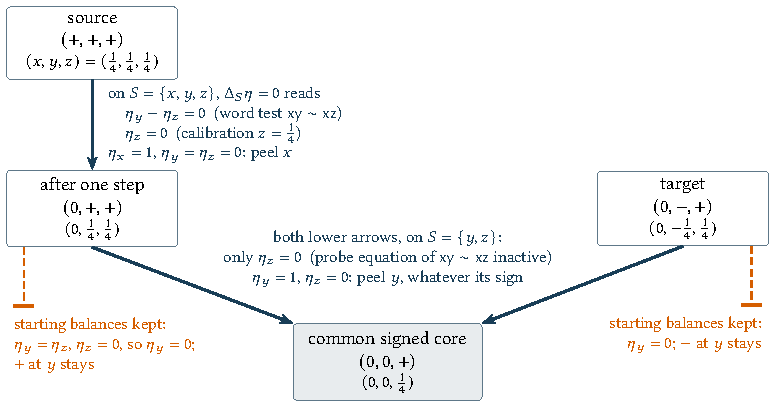
\includegraphics{figures/fig2-peeling.pdf}
  \Description{A flow diagram of signed supports in the coordinate order (x, y, z). The source, with signs (+, +, +) at the point (1/4, 1/4, 1/4), has an arrow to the node after one step, with signs (0, +, +) at (0, 1/4, 1/4); the arrow is labelled with the weight equations on the full support, eta_y - eta_z = 0 from the word test and eta_z = 0 from the calibration, solved by eta_x = 1, eta_y = eta_z = 0, which peels x. The node after one step and the target, with signs (0, -, +) at (0, -1/4, 1/4), both have arrows to the common signed core (0, 0, +) at (0, 0, 1/4). These arrows are labelled: on the support {y, z} only eta_z = 0 remains, because the probe equation of the word test is inactive, and eta_y = 1, eta_z = 0 peels y whatever its sign. Dashed stubs from the intermediate node and the target show what happens if the starting balances are kept. They force eta_y = 0, so the intermediate node retains positive y, the target retains negative y, and the two do not reach a common signed core.}
  \caption{Peeling the staged example of Section~\ref{sec:question}. Nodes
  are signed supports in the coordinate order $(x,y,z)$, each with a point
  that has it; arrow labels give the weight equations $\Delta_S\eta=0$ of
  the tests active on the current support~$S$. Recomputing them after each
  step leads the source (two steps) and the target (one step) to a common
  signed core. After the source's first step, the probe equation of
  $\mathsf{xy}\sim\mathsf{xz}$ is inactive. The dashed stubs keep the balance
  equations from the source support for both reductions. These force
  $\eta_y=0$ on $\{y,z\}$, leaving no common signed support to peel to.}\label{fig:peeling}
\end{figure}

% ---------------------------------------------------------------------------
\subsection{Computing the core}\label{sec:computing-core}

The core is computed by linear programming over recomputed supports. At
a support~$S$, a step removing $j\in S$ exists exactly when
$\Delta_S\eta=0$, $\eta\ge0$, $\eta_j\ge1$ has a rational solution, since
clearing denominators gives integer weights. Each round sums one solution
for each such~$j$, removing all removable coordinates at once, and
then recomputes the active tests. Every round but the last removes a
coordinate. The last can stop at a nonempty support, which has no proper
step and is therefore the core by Lemma~\ref{lem:restriction}(c). No
connectivity computation is needed, and Section~\ref{sec:algorithm} bounds
the cost. For a prescribed survivor set $T\subseteq S$, add $\eta_j=0$ on
$T$ and $\eta_j\ge1$ on $S\setminus T$ to $\Delta_S\eta=0$. This rational
feasibility test is equivalent to the existence of the peeling step
$S\to T$ after clearing denominators.

Related uses of linear programming occur in continuous Petri
nets and exponential families. Fraca and
Haddad's Algorithm~2~\cite{fracahaddad} alternates linear programming for
maximal state-equation support with forward and reverse firing-set
restrictions. For exponential families, Csiszár and
Matúš~\cite{csiszarmatus} characterize the variation closure of canonically
convex families using accessible faces. Geyer~\cite{geyer} uses repeated
linear programming in a method that identifies a limiting conditional model
via a generic direction of recession.

% ---------------------------------------------------------------------------
\subsection{Limits and exact interpolation}\label{sec:limits}

Necessity in Theorem~\ref{thm:core} must exclude sequences with ever finer
steps that pass between signed supports near a common limit point, which
can be irrational. A \defterm{real chart} is the set of points of $\FR$
with a given signed support, and a \defterm{rational chart} the set of
points of $\FQ$ with it.

\begin{lemma}[A chart limit gives a peeling step]\label{lem:limit}
Let points $x^{(k)}\in\RR^J$ satisfy every test of the system and share one
signed support~$\sigma$ with support~$S$, and let $x^{(k)}\to x^*\in\RR^J$.
Then $S\to\supp x^*$ is a peeling step, $x^*$ has the signs of $\sigma$ on
$\supp x^*$, and $\SC(x^*)=\SC(x^{(k)})$.
\end{lemma}

The proof, in Appendix~\ref{app:core-proofs}, takes logarithms on~$S$ and
keeps every test active on~$S$, including tests whose monomials vanish
at~$x^*$. %
Subtracting the bounded correction given by a fixed linear right inverse
produces a kernel vector on the vanishing coordinates. Negating this vector,
approximating in the rational kernel, clearing denominators and extending
by zero on the surviving coordinates yields a weight vector positive
exactly on $S\setminus\supp x^*$. No budget is used. The lemma can also be derived from Tevelev's criterion for
closures of subvarieties of a complex torus~\cite[Lemma~2.2]{tevelev}.
Sufficiency needs the opposite move.

\begin{lemma}[Rational interpolation]\label{lem:interpolation}
Any two points $x,x'\in\FQ$ with the same signed support are finely
connected through feasible rational points with that signed support.
\end{lemma}

The proof, also in Appendix~\ref{app:core-proofs}, samples the log-affine curve $\xi_j(t)=\sgn(x_j)|x_j|^{1-t}|x'_j|^{t}$ through the prime
factorizations of the endpoint ratios $|x'_j|/|x_j|$. Their exponent
vectors lie in the kernel of $\Delta_S$ and vanish on unchanged
coordinates. So the samples satisfy every test exactly, and tight budgets
on unchanged coordinates stay exact.

% ---------------------------------------------------------------------------
\subsection{The classification}\label{sec:classification}

The next lemma, proved in Appendix~\ref{app:core-proofs} and reused in
Section~\ref{sec:timing}, ties sequences with steps below every tolerance
to the connected components of a compact closure.

% seq{}uences: {} breaks the small-caps Qu ligature, which text extraction drops.
\begin{lemma}[Small-step seq{}uences in a compact closure]\label{lem:compact-chain}
Let $Y$ be a dense subset of a compact metric space~$Z$, and let
$h,h'\in Y$. %
The points $h$ and $h'$ lie in the same connected component of~$Z$ if and
only if, for every $\varepsilon>0$, there is a finite sequence in~$Y$ from
$h$ to~$h'$ whose consecutive distances are below~$\varepsilon$.
\end{lemma}

\begin{theorem}[Signed-core classification]\label{thm:core}
Let $J$ be finite. Fix finitely many tests $x^a=c\,x^b$ with
$a,b\in\NN^J$ and $c\in\QQ$, and finitely many $\ell^1$ budgets
$\sum_{j\in J_\beta}|x_j|\le\kappa_\beta$ with rational~$\kappa_\beta$.
Suppose the set $\FQ$ of feasible rational points is bounded. Then
$x,x'\in\FQ$ are finely connected if and only if $\SC(x)=\SC(x')$.
\end{theorem}

\begin{proof}
For sufficiency, iterating Lemma~\ref{lem:restriction}(a) along a peeling
from $\supp x$ to its core finely connects $x$ to a feasible rational
point $\hat x$ with support $\core(\supp x)$ that agrees with $x$ there.
Obtain $\hat x'$ from $x'$ in the same way. Equal signed cores give $\hat x$
and $\hat x'$ the same signed support, so Lemma~\ref{lem:interpolation}
joins them, and reversing the sequence from $x'$ completes the
sufficiency proof.

For necessity, let $\sigma$ range over the finitely many signed supports
of points of~$\FQ$, and let $K_\sigma$ be the closure of the rational chart
of~$\sigma$. Each $K_\sigma$ is compact by rational boundedness. If $K_\sigma$ and
$K_\tau$ meet at~$x^*$, Lemma~\ref{lem:limit} gives both charts the signed
core of~$x^*$. The unions of the sets $K_\sigma$ grouped by signed core
therefore form a finite family of pairwise disjoint compact sets. If at
least two classes occur, take $d>0$ to be the minimum of their pairwise
distances. Every feasible rational point lies in its own class union, so
no sequence with steps below $d$ changes class.
\end{proof}

Thus fine connectivity depends only on the support that survives iterated
peeling and on the signs there, not on magnitudes. The staged example's
endpoint eigenvalue vectors have equal signed cores, so they are finely
connected by Theorem~\ref{thm:core}. In the sign example, the probe
equation $y^2=z^2$ gives $2\eta_y=2\eta_z$, and the calibration gives
$\eta_z=0$. Thus $\{y,z\}$ is irreducible, and the different signs at $y$
give different signed cores. The two eigenvalue vectors are therefore not
finely connected.

Boundedness cannot be dropped. For $xy^2=1$ with no budgets, the balance
$\eta_x+2\eta_y=0$ forces zero weights, so both coordinates survive, and
the endpoints $(1,1)$ and $(1,-1)$ have different signed cores. Yet they
are finely connected: sample the rational points $(t^2,\pm1/t)$ finely
from $t=1$ to $t=n$ on each branch, and cross the gap $2/n<\varepsilon$
between the branches at $t=n$.

\begin{remark}[Components of the rational closure]\label{rem:closure}
Under the hypotheses of Theorem~\ref{thm:core}, the closure
$K=\overline{\FQ}$ is compact, and by Lemma~\ref{lem:compact-chain} points
of $\FQ$ are finely connected exactly when they lie in one component
of~$K$. Every component of $K$ meets~$\FQ$, although density alone would
not show this. Indeed, each point of $K$ lies in the closure of one of the
finitely many rational charts, each rational chart lies in one component
by Lemmas~\ref{lem:interpolation} and~\ref{lem:compact-chain}, and
components are closed. So the components of $K$ are labeled by the signed
cores of points of~$\FQ$. In the terms of Akin and
Wiseman~\cite[Section~3]{akinwiseman}, fine connectivity is the chain
relation of the identity map of $\FQ$ with the sup metric.
\end{remark}

Three objects must be kept apart: the real feasible set $\FR$, whose
components Corollary~\ref{cor:real} classifies; the closure $K$, which can
be strictly smaller; and finite rational sequences, which need no
continuous rational path. For $y^2=2x^2$ with $|x|+|y|\le1$, $K$ is the
origin and $\FR$ is two crossing segments. Under rational boundedness the
real and rational verdicts agree on rational endpoints in this class
(Corollary~\ref{cor:real}); Section~\ref{sec:real-rational} gives
instances with one word-against-pair test where they differ.

Three examples bound the theorem. For $xy=1$ with $|x|+|y|\le3$, the
balance $\eta_x+\eta_y=0$ forces zero weights, so two signed cores
survive, $(+,+)$ and $(-,-)$. The core can be empty even when no weight
vector is positive on the whole support. For $xy=x$ with $|x|+|y|\le2$,
the only proper one-step peel from full support removes~$x$. On $\{y\}$
the row is inactive, so $y$ then peels. Every feasible point has empty
core. Finally, the spherical section of $z_0z_2=z_1^2$ has two components,
while its budgeted affine cone has one signed core, so the theorem is not a
special case of Soprunova and Sottile's component
count~\cite[Theorem~2.4(2)]{soprunovasottile}.

Geometrically, on a fixed support~$S$, consider the damping-factor set
$\{e^{-\eta}:\eta\in\RR_{\ge0}^S,\ \Delta_S\eta=0\}$. With
$d_j=e^{-\eta_j}$, each balance becomes $d^a=d^b$, equivalently two
binomial inequalities on $(0,1]^S$, and the closure of this positive
solution set is a toric cube~\cite[Lemma~1 and Theorems~1--2]{toriccubes}.
Vanishing monomials can make some of these inequalities
vacuous~\cite[Example~3]{toriccubes}.

% ---------------------------------------------------------------------------
\subsection{Real components}\label{sec:real-components}

Over $\RR$ the same signed cores classify the components of the binomial
equations and budgets, with no boundedness at all.

% gloss: real component
\begin{corollary}[Real components]\label{cor:real}
Fix a budgeted signed-binomial system on a finite set~$J$, read over~$\RR$,
and let $\FR$ be its real feasible set, with no boundedness assumed. For
$x,x'\in\FR$ the following are equivalent: (i)~$x$ and $x'$ lie in one
connected component of~$\FR$; (ii)~a continuous path in $\FR$ joins them;
(iii)~$\SC(x)=\SC(x')$. If $\FQ$ is bounded, then for $x,x'\in\FQ$ these
conditions are also equivalent to fine connectivity.
\end{corollary}

\begin{proof}
A path lies in one component, so (ii) implies~(i). For (i)~implies~(iii),
consider the finitely many nonempty real charts. Every finite
limit of a real chart has the same signed core by Lemma~\ref{lem:limit}.
Each core class and its complement are therefore finite unions of chart
closures, so each class is relatively clopen. A connected set thus lies in
one class. For (iii)~implies~(ii), the monomial-curve calculation in the
proof of Lemma~\ref{lem:restriction}(a) applies to real feasible points:
the equations persist and every budget weakly decreases. Peeling $x$ and
$x'$ gives points $\hat x,\hat x'$ with the same signed support. The
log-affine interpolation from the proof of Lemma~\ref{lem:interpolation}
preserves the equations between these real points, and
$|\xi_j(t)|\le(1-t)|\hat x_j|+t|\hat x'_j|$ preserves the budgets.
Concatenating these paths (with the second peeling path reversed) proves~(ii).
The last claim follows from Theorem~\ref{thm:core}.
\end{proof}

Rational boundedness serves only the agreement, and the signed cores
occurring over $\RR$ and $\QQ$ can differ: $x^2=2$ with $|x|\le2$ has two
real components and no rational point. The classification is for binomial
equations: with $y=x^2$, $z=y$ and the affine trinomial $y+z=1$, the real
feasible set is the two points $(\pm1/\sqrt2,1/2,1/2)$, while the binomial
tests alone give both the empty core.

% gloss: P-complete
% gloss: PSPACE-hard
Section~\ref{sec:real-ncl} shows that deciding whether two supplied
feasible rational endpoints lie in the same real path component is
P-complete for binary-encoded budgeted signed-binomial systems under
deterministic log-space many-one reductions. Allowing a growing number of
scalar equations $x_j+y_j=1$ gives PSPACE-completeness under
polynomial-time many-one reductions.


\section{One word against one: the tractable side and profile steps}\label{sec:tractable}

This section proves part~(i) of Theorem~\ref{thm:boundary}, the
fixed-profile criterion, the single-word claims of
Theorem~\ref{thm:directed}, and the P-complete half of
Corollary~\ref{cor:algebraic}.
% gloss: single-word class
We call a model \defterm{single-word}, or in the \defterm{single-word class}, when all its word tests are word-against-word.

% ---------------------------------------------------------------------------
\subsection{From word tests to binomial equations}\label{sec:compile}

Feasibility then splits into three systems with separate variables.

\begin{lemma}[Feasibility separates]\label{lem:separate}
Fix a shared-probe model in the single-word class, a profile $p$ whose held
word tests form an admissible set, and a parameter vector
$(\theta,\alpha,L)$ with tables~$P$. Then the configuration $(p,P)$ is
feasible if and only if conditions (a)--(c) hold.
(a)~The vector $\theta$ satisfies $\theta(w)=\theta(w')$ for every held
word test $w\sim w'$ and $\theta(w)=c\,\theta(w')$ for every held
probability-ratio test.
(b)~The vector $\alpha$ is a feasible point of $\Phi_p$ with its budgets.
(c)~The tables satisfy $L_m(g,h;r,r')>0$ exactly when
$(m,g,r,h,r')\in\Gamma_p$, and $L$ satisfies the block-mass conditions at
every level of~$p$.
\end{lemma}

Lemma~\ref{lem:compile}(a) gives the split
(Appendix~\ref{app:tractable-proofs}). The next lemma moves between steps in the tables and
steps in each part.

\begin{lemma}[Tables and parameters]\label{lem:transfer}
Fix a shared-probe model and put $N=|X||R|$.
\begin{enumerate}
\item[(a)] Any two parameter vectors, with eigenvalue vectors
$\alpha_A,\alpha_B$ and tables $P_A,P_B$, satisfy
$\|\alpha_A-\alpha_B\|_\infty\le(2N/\delta)\,\|P_A-P_B\|_\infty$.
\item[(b)] On the set of parameter vectors, the tables are uniformly
continuous functions of $(\theta,\alpha,L)$.
\item[(c)] At a profile $p$ of the single-word class, let rational vectors
$\theta,\theta'$ satisfy the probability floor, normalization and the
equations of Lemma~\ref{lem:separate}(a). For every rational
$\varepsilon>0$, a finite sequence of such rational vectors with sup-norm
steps below~$\varepsilon$ joins them.
\item[(d)] The same holds for two register tables satisfying
Definition~\ref{def:model} and Lemma~\ref{lem:separate}(c) at~$p$, through
rational affine interpolation.
\end{enumerate}
\end{lemma}

Appendix~\ref{app:tractable-proofs} proves the lemma, interpolating label
probabilities geometrically and registers affinely.

\begin{remark}[The role of each restriction]\label{rem:restrictions}
The $\ell^1$ budget keeps every base kernel positive along the monomial
curves of Lemma~\ref{lem:restriction}(a), which shrink absolute values,
while the eigenvalues themselves can be negative or zero. Positivity of
$Q_m$ alone would not do. On $(\mathbb Z/2)^2$, take two generating
characters and their product as the three probes. Eigenvalues
$(4/5,4/5,7/10)$ give a positive kernel. Damping the third eigenvalue to
zero gives the entry $(1-4/5-4/5)/4=-3/20$. The probability floor
$\theta_m\ge\delta>0$ gives Lemma~\ref{lem:transfer}(a), through division
by~$\theta_m$. Equal word lengths make the rate equations homogeneous, so
normalization preserves them. The register conditions are affine and
separate from the others.
\end{remark}

% ---------------------------------------------------------------------------
\subsection{Proof of the fixed-profile criterion}\label{sec:fixed-proof}

\begin{proof}[Proof of Theorem~\ref{thm:fixed-profile}]
By Lemma~\ref{lem:separate}, the eigenvalue vectors of feasible
configurations at~$p$ are exactly the feasible rational points of $\Phi_p$
with its budgets. The reversal equations belong to $\Phi_p$ because every
parameter vector satisfies them. Every coordinate lies in a budget, so this
feasible rational set is bounded, and Theorem~\ref{thm:core} applies to it.

For necessity, fix a rational $\varepsilon_\alpha>0$ and a reconfiguration
sequence from $A$ to $B$ at tolerance $\delta\varepsilon_\alpha/(2N+1)$,
with $N$ as in Lemma~\ref{lem:transfer}. By Lemma~\ref{lem:transfer}(a),
consecutive eigenvalue vectors differ by less than $\varepsilon_\alpha$ in
sup norm. So $\alpha_A$ and $\alpha_B$ are finely connected, and
Theorem~\ref{thm:core} gives $\SC_p(\alpha_A)=\SC_p(\alpha_B)$.

For sufficiency, fix $\varepsilon>0$ and change one part of the parameter
vector at a time. Lemma~\ref{lem:transfer}(c) joins $\theta_A$ to
$\theta_B$, Theorem~\ref{thm:core} joins $\alpha_A$ to $\alpha_B$, and
Lemma~\ref{lem:transfer}(d) joins $L_A$ to $L_B$, whose positive entries
both give~$\Gamma_p$. Every intermediate configuration is feasible by
Lemma~\ref{lem:separate}. By Lemma~\ref{lem:transfer}(b), fine enough steps
in each part change every table entry by less than~$\varepsilon$.
\end{proof}

% ---------------------------------------------------------------------------
\subsection{The algorithm and its certificates}\label{sec:algorithm}

The linear-programming (LP) computation of Section~\ref{sec:computing-core}
has at most $|J|$ deletion rounds and one final check. Its LPs have
polynomial input size because their matrices are restrictions of the
binary-encoded exponent differences. Neither this computation nor the real
signed-core criterion of Corollary~\ref{cor:real} requires a bounded locus,
so the same computation decides real path-component membership
(Corollary~\ref{cor:real-complexity}). Fraca and Haddad's
Proposition~27~\cite{fracahaddad} analyzes their Algorithm~2
(Section~\ref{sec:computing-core}).

% gloss: Gordan certificate
A peeling sequence shows which coordinates can be removed; a certificate
must also show that no more can be. A \defterm{Gordan certificate} for a
support $C$ is an integer vector $\lambda$, indexed by the tests active
on~$C$, with $\Delta_C^{\mathsf T}\lambda>0$ in every coordinate; for
$C=\emptyset$ it is empty. In the sign example on $C=\{y,z\}$, multiplier $1$ on
the difference vector $(2,-2)$ of $y^2=z^2$, multiplier $3$ on $(0,1)$ of
$z=1/4$, and $0$ on the identity reversal equations give
$\Delta_C^{\mathsf T}\lambda=(2,1)$. Let $D_0$ be the
maximum of $1$ and the absolute values of the entries of the vectors $a-b$.

\begin{theorem}[Polynomial time, with certificates]\label{thm:certificates}
Let $\Phi$ be an explicitly binary-encoded budgeted signed-binomial system
with $n=|J|$ coordinates and $|\Phi|$
tests.
\begin{enumerate}
\item[(a)] For every support $S$, the core $\core_\Phi(S)$ is computable in
deterministic polynomial time.
\item[(b)] Integer weight vectors of a peeling sequence from $S$ to~$C$,
each checked against the tests active at its own support, together with a
Gordan certificate for $C$, prove $C=\core_\Phi(S)$. Such a certificate
exists with at most $n$ stages and at most $n$ nonzero multipliers, each
of absolute value at most $n!\,D_0^n$. It can be stored with binary length
$O(n^3(1+\log(n+1)+\log D_0)+n\log(|\Phi|+1))$.
% gloss: polynomial-size certificates (G8; read back after the proof)
\item[(c)] Fine Reachability at a fixed profile in the single-word class is
decided in deterministic polynomial time, and both answers have
polynomial-size certificates, checkable in polynomial time.
\end{enumerate}
\end{theorem}

\begin{proof}
Part~(a) is the computation above. Appendix~\ref{app:tractable-proofs}
proves the bounds and~(b)--(c). In~(b), soundness uses the terminal
dot-product check and completeness uses Gordan's alternative. Part~(c)
compiles $\Phi_p$, applies Theorem~\ref{thm:fixed-profile} and gives the
verifier for both verdicts.
\end{proof}

Thus both answers are certified by peeling stages and Gordan certificates,
not by the points of a sequence.

Checking whether a supplied rational point satisfies the binomial equations
of a Fine Connectivity instance is a separate task. After handling zero
coefficients, vanishing monomials and signs, clear denominators in each
comparison, keeping the powers encoded. Proposition~2.1 of Etessami,
Stewart and
Yannakakis~\cite[Proposition~2.1]{etessamistewartyannakakis} supplies the
power-product equality check. With the zero and sign checks and
rational budget arithmetic, this equality check verifies feasibility of the
supplied endpoint. Boundedness remains a promise, and the check does not
decide whether a feasible point exists.

\begin{proposition}[Explicit seq{}uences can need exponential binary length]\label{prop:long-sequences}
For $k\ge1$, let $\Phi$ have coordinates $x_0,\dots,x_k$, tests
$x_{i+1}=x_i^2$ for $0\le i<k$, and budgets $|x_i|\le1$. The points $0$
and $(1,\dots,1)$ are finely connected. Every sequence of feasible rational
points between them with sup-norm steps below $1/4$ contains a point whose
coordinate $x_k$ has a reduced denominator of binary length at least
$2^k+1$.
\end{proposition}

The proof (Appendix~\ref{app:tractable-proofs}) follows~$x_0$ across
$[1/4,1/2)$.

\paragraph{Scope of the tolerance.} The single-word P-completeness result
and its certificates concern fine reachability, at every positive rational
tolerance. Different signed cores can still be joined at a coarse
tolerance, as one step joins the two signs of the sign example above~$1/8$. Proposition~\ref{prop:separation} supplies a
sufficient separation cutoff whose expanded rational denominator can
require exponentially many binary digits. For each NCL reduction instance
of Section~\ref{sec:hard}, the NCL verdict agrees with sequence existence
at its supplied cutoff and at every smaller positive tolerance. A positive
certificate proves sequence existence at every tolerance, while by
Proposition~\ref{prop:long-sequences} an explicit sequence can require
exponentially many binary digits even at a fixed tolerance.

% ---------------------------------------------------------------------------
\subsection{P-hardness}\label{sec:p-hardness}

% gloss: anchor
As in both examples of Section~\ref{sec:question}, $\mathsf z$ is the
\defterm{anchor}, a label calibrated to $1/4$ whose coordinate never peels.
We reduce from monotone circuit value, which Goldschlager proved P-complete
under log-space reductions~\cite{goldschlager}; Greenlaw, Hoover and Ruzzo
prove the variant with numbered gates and assigned
inputs~\cite[Theorem~6.2.2]{greenlawhooverruzzo}. A circuit lists gates
$1,\dots,G$, each a constant $0$ or $1$ or a binary AND or OR of earlier
gates, and names an output gate~$\gamma_{\mathrm{out}}$.

% gloss: sentinel
The reduction outputs an instance of the single-word class with base
$\{0,1\}$, one probe, a one-value register and only level~$0$. Its labels,
each its own reversal, are a gate label $\mathsf g_\gamma$ for each gate,
the anchor and a \defterm{sentinel}~$\mathsf s$, whose sign alone
distinguishes the two endpoints. The eigenvalues of the gate labels, the anchor and the sentinel are
$g_\gamma$, $z$ and~$s$, respectively. With $\delta=1/(G+2)$ every label
probability is~$\delta$; also $\kappa=1/2$ and $H=3$. To keep two tests per
gate uniformly for log-space output, each gate receives two named word tests,
its \emph{slots}. An AND gate uses one test per input, constant~$0$ and OR
repeat one test, and constant~$1$ uses two trivial identities so it still
fills both slots. With inputs $\gamma',\gamma''$, the slots are
\[
\begin{array}{lll}
\text{constant }0: & \mathsf g_\gamma\mathsf{zz}\sim\mathsf{zzz}, & \mathsf g_\gamma\mathsf{zz}\sim\mathsf{zzz};\\
\text{constant }1: & \mathsf{zzz}\sim\mathsf{zzz}, & \mathsf{zzz}\sim\mathsf{zzz};\\
\text{AND}: & \mathsf g_\gamma\mathsf g_{\gamma'}\mathsf z\sim\mathsf z\mathsf g_{\gamma'}\mathsf z, &
\mathsf g_\gamma\mathsf g_{\gamma''}\mathsf z\sim\mathsf z\mathsf g_{\gamma''}\mathsf z;\\
\text{OR}: & \mathsf g_\gamma\mathsf g_{\gamma'}\mathsf g_{\gamma''}\sim\mathsf z\mathsf g_{\gamma'}\mathsf g_{\gamma''}, &
\mathsf g_\gamma\mathsf g_{\gamma'}\mathsf g_{\gamma''}\sim\mathsf z\mathsf g_{\gamma'}\mathsf g_{\gamma''}.
\end{array}
\]
The output test is
$\mathsf{ss}\mathsf g_{\gamma_{\mathrm{out}}}\sim\mathsf{zz}\mathsf g_{\gamma_{\mathrm{out}}}$.
All $2G+1$ word tests and the calibration $z=1/4$ are held, and the only
admissible set is the set of all word tests. The endpoint $A$ has every
eigenvalue $1/4$, and $B$ differs only in $s=-1/4$; both are feasible
whatever the circuit, since $s$ enters only the output test, squared.

In other words, a test is active only while all its letters are nonzero.
So the coordinates that peel follow gate-local Horn rules: a constant~$1$
is removed, an AND gate once both inputs are, an OR gate once either is,
and $s$ once the output gate is. In the three-gate circuit, $\mathsf g_1$
is the constant~$0$, $\mathsf g_2$ the constant~$1$, and the output is
$\mathsf g_3=\mathrm{OR}(\mathsf g_1,\mathsf g_2)$. Here $g_2$ peels first,
making the test of $\mathsf g_3$ inactive; then $g_3$ peels, making the
output test inactive; then $s$ peels. The core is $\{z,g_1\}$, and
$B$ is finely reachable from~$A$. With AND in place of OR, the slot of
$\mathsf g_1$ keeps $g_3=z$ after $g_2$ leaves. Then $\{z,g_1,g_3,s\}$ is
irreducible and $B$ is not finely reachable, although one numerical step
joins the endpoints at any tolerance above $1/20$.

\begin{theorem}[P-hardness]\label{thm:p-hard}
The map from a monotone circuit to the instance above is computable in
deterministic logarithmic space. The configurations $A$ and $B$ are
feasible at one common profile with full table support, and $B$ is finely
reachable from $A$ if and only if the circuit outputs~$1$. Hence Fine
Reachability at a fixed profile in the single-word class is P-hard under
deterministic log-space many-one reductions on promised-feasible inputs.
\end{theorem}

\begin{proof}[Proof sketch]
An active gate test other
than a constant-$1$ slot gives $\eta_{g_\gamma}=\eta_z$, where $\gamma$ is
its gate. The constant-$1$ slots are identities. The active output test
gives $2\eta_s=2\eta_z$, and the calibration gives $\eta_z=0$. The anchor,
the false gates and, if the output is~$0$, the sentinel form an irreducible
support, so they lie in the core of the full support
(Lemma~\ref{lem:irreducible}). A first true gate in that core would peel
alone, and so would the sentinel once the output gate is gone. So the
signed cores of $A$ and~$B$ agree exactly when the output is~$1$, and
Theorem~\ref{thm:fixed-profile} gives the equivalence.
Appendix~\ref{app:tractable-proofs} gives the details and the log-space
transducer.
\end{proof}

Thus the sentinel survives peeling exactly when the circuit outputs~$0$.
With
Theorem~\ref{thm:certificates}, the problem is P-complete, and since the
reductions land inside the promise, it is in log-space-uniform NC only if P
equals log-space-uniform NC.

The reduction follows the circuit-value pattern of Fraca and Haddad's
Proposition~32 for continuous Petri nets~\cite{fracahaddad}. Here the
surviving signed core computes the circuit. For a given gate count, the
endpoint eigenvalue vectors are fixed independently of the gate types,
wiring and output value; the endpoints share a profile within each
instance and differ only in one sign. On these instances the removed set
is the least model of the gate-local Horn rules above, which the
propagation of Dowling and Gallier computes in linear
time~\cite[Sections~4--5]{dowlinggallier}. This reading is for the circuit
instances only: in general a peeling step combines tests through kernel
vectors found by linear programming.

% ---------------------------------------------------------------------------
\subsection{Profile steps: the directed criterion}\label{sec:directed}

% gloss: profile order
% gloss: cover
% gloss: profile step
Theorem~\ref{thm:directed} lets the profile change: a configuration can
acquire held tests, refine its register partitions or shrink its table
support, but never the reverse, so a held test keeps passing for the rest
of the sequence. Definition~\ref{def:profile-steps} extends the sequences and fine
reachability of Section~\ref{sec:profiles}.

\begin{definition}[Profile order and profile steps]\label{def:profile-steps}
For profiles $p$ and~$q$, put $p\preceq q$ if $\Gamma_q\subseteq\Gamma_p$,
$F^q_\ell$ refines $F^p_\ell$ at every level~$\ell$, and
$\mathcal T_p\subseteq\mathcal T_q$. An attained profile $q$ \emph{covers}
an attained $p$ if $p\prec q$ and no attained profile lies strictly between.
A \emph{numerical step} at tolerance~$\varepsilon$ joins feasible
configurations $A,B$ with $p_A=p_B$ and $\|P_A-P_B\|_\infty<\varepsilon$.
A \emph{profile step} joins feasible configurations $A,B$ such that $p_B$
covers $p_A$ and either $\Gamma_{p_B}=\Gamma_{p_A}$ and $P_B=P_A$, or
$\Gamma_{p_B}\subsetneq\Gamma_{p_A}$ and the projected tables
$\theta_mQ_m(g,h)$ agree. A \emph{reconfiguration sequence at
tolerance~$\varepsilon$} is a finite, possibly empty, sequence of such
steps through feasible rational configurations. $B$ is \emph{finely
reachable} from $A$ if one exists from $A$ to $B$ for every rational
$\varepsilon>0$.
\end{definition}

In other words, steps go up the partial order~$\preceq$, and agreement of
the projected tables means $\theta_B=\theta_A$ and $\alpha_B=\alpha_A$, so
only the register can change. %
In the sign example the two labels are self-reversing. Take $\kappa=1/2$,
$H=2$, full table support and only level~$0$. The admissible sets of word tests are the empty set and the
singleton containing $\mathsf{yy}\sim\mathsf{zz}$. Let $A$ hold only
the calibration, at $y=1/4$, and let $B$ also hold
$\mathsf{yy}\sim\mathsf{zz}$, at $y=-1/4$; then $p_A\preceq p_B$.

\begin{center}
\fbox{\begin{minipage}{0.93\linewidth}
\textsc{Fine Reachability with profile steps}\par\smallskip
\emph{Input:} an explicitly presented model, and two rational configurations
$A$ and~$B$, each given by its profile, or data that determine it
(Remark~\ref{rem:readback}), and its parameter vector or transition tables,
in binary.\par\smallskip
\emph{Promise:} $A$ and $B$ are feasible.\par\smallskip
\emph{Question:} is $B$ finely reachable from~$A$?\par\smallskip
\emph{Supplied-tolerance variant:} the input also contains
$\varepsilon_0\in\QQ_{>0}$, and the question is whether a reconfiguration
sequence at tolerance~$\varepsilon_0$ exists.
\end{minipage}}
\end{center}

\begin{lemma}[One change per profile step]\label{lem:covers}
If $q$ covers $p$, then $q$ differs from $p$ in exactly one of the
following: the table support; the held word tests; the held value tests;
the partition at one level. If the held value tests differ, $q$ holds
exactly one more value test than~$p$.
\end{lemma}

Appendix~\ref{app:tractable-proofs} proves the lemma by building an attained
profile, above $p$ and at most~$q$, that changes one part. So every step has one of six types: numerical; support;
word-test; value-test; partition at a non-final level; partition at the
final level. Only a word-test cover can add more than one test. In that
case no admissible set of word tests lies strictly between the two held
word-test sets.

\begin{theorem}[Directed criterion]\label{thm:directed}
Fix a shared-probe model in the single-word class, and let $A$ and $B$ be
feasible rational configurations. Then $B$ is finely reachable from $A$ if
and only if $p_A\preceq p_B$ and $\SC_{p_A}(\alpha_A)=\SC_{p_A}(\alpha_B)$,
where both signed cores are computed from the eigenvalue constraints
$\Phi_{p_A}$ of the source profile, including the reversal equations. Fine
Reachability with profile steps in this class is P-complete under
deterministic log-space many-one reductions, and both answers have
polynomial-size certificates, checkable in polynomial time, that include
the order comparison. For models in which exactly one word test is
word-against-pair and all others are word-against-word, Fine Reachability
with profile steps is PSPACE-hard under polynomial-time many-one
reductions.
\end{theorem}

Thus profile steps add only the order condition $p_A\preceq p_B$, and both
cores come from the source's constraints; the sign example below shows why
the target's constraints would not do.

\begin{proof}[Proof outline]
Steps never lower the profile, so every later configuration passes the
tests of~$p_A$, and profile steps preserve~$\alpha$; necessity then follows as
for Theorem~\ref{thm:fixed-profile}. For sufficiency, combine the target's
label probabilities and eigenvalues with the source register at~$p_A$, and
reach that configuration by Theorem~\ref{thm:fixed-profile}. Then climb a
saturated chain of attained profiles at these values, interpolating to the
upper register at the lower profile before each cover with unchanged
support. Appendix~\ref{app:tractable-proofs} gives the details and proves
the complexity claims.
\end{proof}

In the sign example, $\Phi_{p_A}$ gives only $\eta_z=0$, so $y$ peels and
both signed cores are $z$ alone: $B$ is finely reachable from~$A$, through
$y=0$. At this calibration-only profile, every feasible eigenvalue vector
has signed core $\{z\}$ with positive sign. Thus every feasible target at
or above that profile is finely reachable from any feasible source there,
by Theorem~\ref{thm:directed}. Using the target's constraints for both cores would add
$2\eta_y=2\eta_z=0$, incorrectly ruling out fine reachability from $A$ to
$B$. Let $A^+$ hold the test at the parameter vector of~$A$. From $A^+$ the
cores differ in the sign of~$y$, so $B$ is not finely reachable; the exact
threshold $1/8$ of Section~\ref{sec:question} is for this pair. No
sequence leads from $A^+$ back to $A$ at any tolerance: reachability is
between configurations, not parameter vectors.

The same sign obstruction persists in a model with a nontrivial register and
four labels. On the staged example's base, register values and labels, take
label probabilities $1/4$ and the common full-support profile holding
$\mathsf{yy}\sim\mathsf{zz}$ and $z=1/4$. Take eigenvalues
$(x,y,z,f)=(-1/8,\pm1/4,1/4,1/8)$, the register redrawn from $\nu$ at every
step, and one block at every level. Then Lemma~\ref{lem:transfer}(a), with
$N=8$ and $\delta=1/8$, excludes every sequence between the two signs at
tolerance $1/272$, a sufficient tolerance rather than the exact threshold.
At the same profile, a direct step between these endpoints changes a table
entry by at most $1/64$, so it is allowed at any tolerance above $1/64$.

Both conditions of Theorem~\ref{thm:directed} can be evaluated from the
full-state labeled transition tables, decision availability at each level,
and held-test membership recorded in Remark~\ref{rem:readback}
(Appendix~\ref{app:tractable-proofs}).

The ordinary and signed row sums in Lemma~\ref{lem:transfer}(a) give $\theta_m$ and $\theta_m\alpha_{mi}$. Dividing by the positive label probability yields $\alpha_{mi}$, so the tables determine both types of value test; Appendix~\ref{app:tractable-proofs}
reconstructs the rest of the configuration.

% ---------------------------------------------------------------------------
\subsection{The algebraic form, first half, and the circuit transfer}\label{sec:circuit-transfer}

Section~\ref{sec:algorithm} and Theorem~\ref{thm:core} give the upper
bound in Corollary~\ref{cor:algebraic}, under the promise that $\FQ$ is
bounded. For hardness, the transducer of Section~\ref{sec:p-hardness} emits
only the eigenvalue tests, budgets $|x_m|\le1/2$ and endpoint
eigenvalue vectors; the resulting instances meet the promises
(Appendix~\ref{app:tractable-proofs}). By Corollary~\ref{cor:real}, which
needs no boundedness, these instances also give the P-hardness in
Corollary~\ref{cor:real-complexity}.


\section{One word against two: the hard side}\label{sec:hard}

% gloss: One Word Against Two
This section proves part~(ii) of Theorem~\ref{thm:boundary}, the
PSPACE-hard half of Corollary~\ref{cor:algebraic},
Corollary~\ref{cor:real-complexity} on real path components and
Theorem~\ref{thm:rational-roots}.
In the shared-probe hardness reductions, exactly one word test compares one
word with two distinct words, and all other word tests compare single
words. With the specified probability floor and load-label calibrations,
the widened test forces a fixed positive sum at every probe. In the
constraint-logic reduction, each edge has its own probe, and either nonzero
summand makes its labeled end available as the tail.

% ---------------------------------------------------------------------------
\subsection{The load test}\label{sec:engine}

For the \defterm{load label}~$\mathsf u$ and labels $\mathsf x,\mathsf y$ we write $u_i$, $x_i$ and $y_i$
for their eigenvalues at probe~$i$.

% Lean: SingleAdditiveLicence.joint_words_iff (the 1+|I| equations), and
% the rate forcing in nclInstrument's legality proof.
\begin{lemma}[The load test]\label{lem:engine}
Let a shared-probe model have distinct labels $\mathsf u,\mathsf x,\mathsf
y$ among its $|M|$ labels, with probability floor $\delta=1/(|M|+1)$, and
let $k>0$ be rational. A parameter vector passes the word test
$\mathsf{uu}\sim\{\mathsf{xu},\mathsf{yu}\}$ and the calibrations
$u_i=k/2$ $(i\in I)$ if and only if $\theta_{\mathsf u}=2\delta$,
$\theta_m=\delta$ for every other label~$m$, $u_i=k/2$ and
\begin{equation}\label{eq:load}
  x_i+y_i=k\qquad\text{for every }i\in I.
\end{equation}
\end{lemma}

\begin{proof}
By Lemma~\ref{lem:compile}(b) the test says
$\theta_{\mathsf u}^2=(\theta_{\mathsf x}+\theta_{\mathsf y})\theta_{\mathsf u}$
and $\theta_{\mathsf u}^2u_i^2=\theta_{\mathsf u}(\theta_{\mathsf
x}x_i+\theta_{\mathsf y}y_i)u_i$ for $i\in I$. Since
$\theta_{\mathsf u}\ge\delta>0$, the first gives
$\theta_{\mathsf u}=\theta_{\mathsf x}+\theta_{\mathsf y}\ge2\delta$. The
other $|M|-1$ label probabilities are at least~$\delta$, and these lower
bounds sum to $(|M|+1)\delta=1$, so normalization forces equality
throughout. With $u_i=k/2>0$, the probe equations become
$\delta^2k^2=\delta^2k(x_i+y_i)$. The converse is the same computation.
\end{proof}

% gloss: load equation
In other words, with the label probabilities forced, each of the $|I|$
probe equations of the test becomes the \defterm{load equation}
\eqref{eq:load}, an affine trinomial in the eigenvalues. Since $k>0$, the
two summands never vanish together: a zero summand forces the other to
equal~$k$, although both may be nonzero in between
(Figure~\ref{fig:mechanism}(b)). %
In Figure~\ref{fig:mechanism}(a), setting $x=0$ makes both monomials
vanish, so $xy=xz$ ceases to constrain~$y$. By contrast, the held, calibrated load
equation $x_i+y_i=k>0$ retains its constraint when either summand
vanishes. Further tests decide which points of each load line are feasible,
and the number of probes grows with the input.

% ---------------------------------------------------------------------------
\subsection{The construction}\label{sec:construction}

% gloss: NCL
We reduce from nondeterministic constraint logic
(NCL)~\cite{hearndemaine}. An AND/OR constraint graph is a finite
multigraph $(V,E)$ whose edges have weights $\wt(e)\in\{1,2\}$ and labeled
ends $v_e^0,v_e^1$; each vertex meets incident weights $2,1,1$ (AND) or
$2,2,2$ (OR). Let $W(v)$ sum the weights over the ends at~$v$, so a loop
counts twice. An orientation $\sigma:E\to\{0,1\}$ makes $v_e^{\sigma(e)}$
the tail of $e$ and the other end its head. The orientation is legal if the heads at
every vertex carry weight at least two (minimum inflow two). Equivalently, since each end is a head or a
tail, the tails at every vertex~$v$ carry weight at most $W(v)-2$. A
flip reverses one edge between legal orientations. Hearn and
Demaine~\cite[Section~2 and Corollary~6]{hearndemaine} prove that deciding
whether flips lead from one supplied legal orientation to another is
PSPACE-hard, and their reduction produces distinct endpoints.

\begin{figure}[tbp]
  \centering
  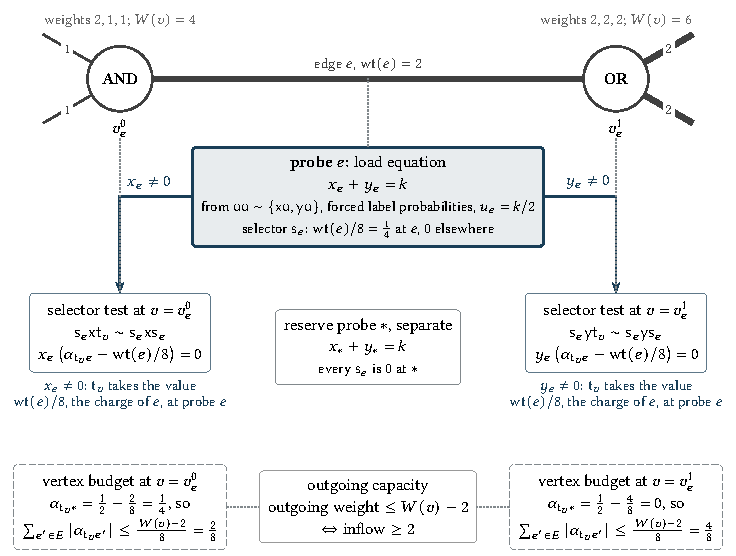
\includegraphics{figures/fig3-ncl-gadget.pdf}
  \Description{A gadget diagram. An AND vertex v_e^0 with edge weights 2, 1, 1 and an OR vertex v_e^1 with edge weights 2, 2, 2 are joined by the edge e of weight 2. The central box shows the load equation x_e + y_e = k at probe e, obtained from the word-against-pair test, the forced label probabilities and the calibration u_e = k/2. The selector s_e has eigenvalue wt(e)/8 = 1/4 at probe e and zero elsewhere. The arrow labelled x_e nonzero leads to the selector equation x_e (alpha_{t_{v_e^0}, e} - wt(e)/8) = 0 at the AND vertex. The arrow labelled y_e nonzero leads to y_e (alpha_{t_{v_e^1}, e} - wt(e)/8) = 0 at the OR vertex. The reserve probe has its own load equation, and every selector has eigenvalue zero there. The dashed boxes show reserve calibrations 1/4 at the AND vertex and 0 at the OR vertex, leaving edge-probe budgets 2/8 and 4/8, respectively. On a canonical orientation lift, each budget is equivalent to outgoing weight at most W(v) - 2, hence to inflow at least 2.}
  \caption{One NCL edge becomes one probe, on which the two summand eigenvalues share the load~$k$. A nonzero summand requires the vertex label at that end of the edge to take the value $\wt(e)/8$, the \emph{charge} of~$e$, at probe~$e$.
% gloss: charge
On a canonical orientation lift, the vertex budget is equivalent to NCL's minimum inflow of two; for an arbitrary feasible configuration, every orientation obtained by choosing one nonzero summand at each edge satisfies minimum inflow two at every vertex. Here the edge~$e$, of weight two, joins an AND vertex $v_e^0$ (edge weights $2,1,1$) to an OR vertex $v_e^1$ (edge weights $2,2,2$); an edge between an AND vertex and an OR vertex always has weight two. The selector $\mathsf s_e$ has eigenvalue $\wt(e)/8$ at probe~$e$ and $0$ at every other probe. The forced label probabilities give the two words of each selector test equal word probabilities, so after cancelling $\wt(e)/8$ the tests $\mathsf s_e\mathsf x\mathsf t_{v_e^0}\sim\mathsf s_e\mathsf x\mathsf s_e$ and $\mathsf s_e\mathsf y\mathsf t_{v_e^1}\sim\mathsf s_e\mathsf y\mathsf s_e$ give the selector equations shown.
% gloss: selector equations
The calibration of $\mathsf t_v$ at the reserve probe~$\ast$ leaves the budget $\sum_{e'\in E}|\alpha_{\mathsf t_ve'}|\le(W(v)-2)/8$, which is $1/4$ at the AND vertex and $1/2$ at the OR vertex. The reserve probe carries its own load equation and no selector. Together with the forced label probabilities, the calibrations and the remaining model constraints, including all per-label budgets, the displayed equations characterize the feasible configurations.}\label{fig:ncl}
\end{figure}

% gloss: reserve probe
% gloss: load label
% gloss: summand labels
% gloss: selector labels
% gloss: vertex labels
Given a graph and legal orientations $\sigma,\tau$, the reduction outputs
the following model. The probes are $I=E\sqcup\{\ast\}$, one per edge and a
\defterm{reserve probe}~$\ast$ for the unused part of each vertex
budget~\eqref{eq:vertex-budget}. The base is $X=\mathbb F_2^d$ with
$d=\lceil\log_2(|E|+2)\rceil$, and
$\chi_i(g)=(-1)^{a_i\cdot g}$ for distinct nonzero $a_i\in X$. The labels,
each its own reversal, are the load label~$\mathsf u$; the
\defterm{summand labels} $\mathsf x,\mathsf y$, which choose tails;
\defterm{selector labels} $\mathsf s_e$ $(e\in E)$, which read the summands
at probe~$e$; and \defterm{vertex labels} $\mathsf t_v$ $(v\in V)$. So
$|M|=|E|+|V|+3$, and we put
\[
  \delta=\frac1{|M|+1},\qquad k=\frac1{4|I|},\qquad\kappa=\frac12,\qquad
  H=3,
\]
with a one-value register and only level~$0$. The value tests are the
calibrations
\[
  u_i=\frac k2\ \ (i\in I),\qquad
  \alpha_{\mathsf s_ei}=
  \begin{cases}\wt(e)/8,&i=e,\\0,&i\neq e,\end{cases}\qquad
  \alpha_{\mathsf t_v\ast}=\frac12-\frac{W(v)-2}8 .
\]
The word tests are the load test and two \defterm{selector tests} per
edge:
\[
  \mathsf{uu}\sim\{\mathsf{xu},\mathsf{yu}\},\qquad
  \mathsf s_e\mathsf x\mathsf t_{v_e^0}\sim\mathsf s_e\mathsf x\mathsf s_e,
  \qquad
  \mathsf s_e\mathsf y\mathsf t_{v_e^1}\sim\mathsf s_e\mathsf y\mathsf s_e .
\]
The only admissible set is the full word-test list. The profile $p$ has
full table support and holds every test.

% gloss: charge
% gloss: selector equations
% gloss: vertex budgets
We call $\wt(e)/8$ the \defterm{charge} of~$e$; the vertex budgets below
cap the tails' total charge at each vertex, as legality caps their weight. The selector tests give the
\defterm{selector equations}~\eqref{eq:selector} below: the vertex label at
an end of~$e$ takes the charge at probe~$e$ whenever that end's summand is
nonzero (Figure~\ref{fig:ncl}). The \defterm{canonical orientation lift} $A_\sigma$ of
$\sigma$ has label probabilities $2\delta$ at $\mathsf u$ and $\delta$
elsewhere, the calibrated eigenvalues, $(x_\ast,y_\ast)=(k,0)$, and
$(x_e,y_e)$ equal to $(k,0)$ or $(0,k)$ as $\sigma(e)$ is $0$ or~$1$. Its
label $\mathsf t_v$ takes the charge of~$e$ at probe~$e$ if $v$ is the
tail of~$e$, and $0$ otherwise. The reduction outputs the model, $p$,
$A_\sigma$, $A_\tau$ and, for the supplied-tolerance variant,
$\varepsilon_0=\delta k/(2|X|+1)$; it runs in polynomial time
(Appendix~\ref{app:ncl-size}).

% ---------------------------------------------------------------------------
\subsection{Feasible configurations}\label{sec:feasible}

The next lemma lists exactly what feasibility at~$p$ requires.

\begin{lemma}[Feasible configurations]\label{lem:feasible}
In the construction of Section~\ref{sec:construction}, a rational parameter
vector gives a feasible configuration at~$p$ if and only if it satisfies
the conditions below and the remaining model constraints. These include
the calibrations and the $\ell^1$ budget of every label. The conditions
are $\theta_{\mathsf u}=2\delta$ and $\theta_m=\delta$ for $m\neq\mathsf
u$, the load equation~\eqref{eq:load} at every probe, the selector
equations
\begin{equation}\label{eq:selector}
  x_e\Bigl(\alpha_{\mathsf t_{v_e^0}e}-\frac{\wt(e)}8\Bigr)=0,\qquad
  y_e\Bigl(\alpha_{\mathsf t_{v_e^1}e}-\frac{\wt(e)}8\Bigr)=0\qquad(e\in E)
\end{equation}
% gloss: vertex budgets
and the \defterm{vertex budgets}
\begin{equation}\label{eq:vertex-budget}
  \sum_{e\in E}|\alpha_{\mathsf t_ve}|\le\frac{W(v)-2}8\qquad(v\in V).
\end{equation}
\end{lemma}

\begin{proof}
The register, support, reversal and admissibility conditions hold here by
construction, so feasibility means Definition~\ref{def:model} and every
held test. Lemma~\ref{lem:engine} handles the load test and the
calibrations of~$\mathsf u$. In a selector test both words have three
labels of probability~$\delta$, and at probe~$i$
Lemma~\ref{lem:compile}(a) requires
$\alpha_{\mathsf s_ei}x_i\alpha_{\mathsf t_{v_e^0}i}=\alpha_{\mathsf
s_ei}^2x_i$. Both sides vanish for $i\neq e$; at $i=e$, cancelling
$\wt(e)/8>0$ gives~\eqref{eq:selector}, and likewise with~$\mathsf y$.
Since $\alpha_{\mathsf t_v\ast}\ge0$, the budget of $\mathsf t_v$
is~\eqref{eq:vertex-budget}.
\end{proof}

The listed equations alone do not suffice: the reserve pair
$(x_\ast,y_\ast)=(1,k-1)$ satisfies all of them but violates the budget
of~$\mathsf x$.

% gloss: available
% gloss: represented
To read orientations off a feasible configuration at~$p$, call the end
$v_e^0$ of $e$ \defterm{available} if $x_e\neq0$, and $v_e^1$ if $y_e\neq0$. An
orientation is \defterm{represented} if the tail of every edge is
available. By~\eqref{eq:load} every edge has an available end, and since
both summands may be nonzero, a feasible configuration can represent
several orientations. On a canonical orientation lift, the vertex budget is
equivalent to minimum inflow two. At any feasible configuration, each
represented outgoing edge forces its full charge in a distinct probe
coordinate at its chosen vertex, so every mixture of represented choices is
legal. Hence two orientations represented by one configuration are joined
by legal flips through orientations it represents. The lift $A_\sigma$
represents only~$\sigma$, so distinct orientations give distinct feasible
endpoints (Appendix~\ref{app:ncl-transfer}).

% ---------------------------------------------------------------------------
\subsection{Both directions of the transfer}\label{sec:transfer}

Fix an instance of the construction. It remains to decode sequences into
legal flips and to lift flips to sequences. Decoding must handle every
feasible step below~$\varepsilon_0$, including
steps that change many coordinates or pass through negative summands, and
configurations representing several orientations.

% Lean: ConstraintLogic common_orientation, flips_of_represents,
% legal_of_represents.
\begin{lemma}[Small steps share an orientation]\label{lem:decode}
Let $A$ and $B$ be feasible configurations at~$p$ whose summands satisfy
$|x_{A,e}-x_{B,e}|<k$ for every $e\in E$. Then some orientation is
represented by both. Hence, if consecutive configurations of a
reconfiguration sequence from $A_\sigma$ to $A_\tau$ satisfy this bound,
legal flips lead from $\sigma$ to~$\tau$.
\end{lemma}

% Lean: Graph.flip_segments_lawful; the encoder clips the summands to
% [0,k], which is the identity on the three segments.
\begin{lemma}[Legal flips lift]\label{lem:lift}
If $\tau$ arises from a legal orientation $\sigma$ by one legal flip, then
for every rational $\varepsilon>0$ a reconfiguration sequence at
tolerance~$\varepsilon$ leads from $A_\sigma$ to~$A_\tau$.
\end{lemma}

% Lean: ncl_chain_iff (at the supplied cutoff) and ncl_fine_iff (fine
% reachability); the smaller-tolerance case combines them with
% monotonicity in writing.
\begin{lemma}[The cutoff]\label{lem:cutoff}
Let $\sigma,\tau$ be legal orientations. For every rational $0<\varepsilon\le\varepsilon_0$ the
following are equivalent: legal flips lead from $\sigma$ to~$\tau$;
$A_\tau$ is finely reachable from~$A_\sigma$; a reconfiguration sequence at
tolerance $\varepsilon$ leads from $A_\sigma$ to~$A_\tau$.
\end{lemma}

\begin{proof}[Proof idea for Lemmas~\ref{lem:decode}--\ref{lem:cutoff}]
At an edge, disjoint available ends at $A$ and $B$ would make $x_e$ jump
between $0$ and~$k$, by~\eqref{eq:load}. Choosing a common available end at
each edge gives a common represented orientation, whatever the signs.
At the forced label probabilities, summing a row for label~$m$ with
weights $\chi_i(g)\chi_i(h)$ gives $\theta_m\alpha_{mi}$. A step below
$\varepsilon_0$ therefore changes each eigenvalue by less than
$|X|\varepsilon_0/\delta<k$, so adjacent configurations share an available
end at every edge. To lift a flip with distinct tails, preload the new tail, interpolate
the summands, and unload the old tail. Each preloaded vertex total is the
larger of its two endpoint totals. For a loop, keep its one charge fixed
and interpolate only the summands. For the cutoff, any sequence at $0<\varepsilon\le\varepsilon_0$ is also one at
$\varepsilon_0$ and decodes to legal flips. Conversely, legal flips lift to
sequences at every positive tolerance.
Appendix~\ref{app:ncl-transfer} gives the full argument.
\end{proof}

As noted after Theorem~\ref{thm:boundary}, this agreement can fail at
larger tolerances.

% ---------------------------------------------------------------------------
\subsection{Length one, and the proof of Theorem~\ref{thm:boundary}(ii)}\label{sec:length-one}

% Lean: the `short` parameter of nclInstrument and of every ncl_* theorem
% gives each length separately; the cancellation is written.
\begin{proposition}[A word-against-pair test of length one]\label{prop:length-one}
Replace $\mathsf{uu}\sim\{\mathsf{xu},\mathsf{yu}\}$ by
$\mathsf u\sim\{\mathsf x,\mathsf y\}$ in the construction, keeping every
other input, including the held load calibrations, $H=3$ and both
endpoints. Then the feasible
configurations at~$p$, and hence the reconfiguration sequences at every
tolerance, are unchanged.
\end{proposition}

\begin{proof}
By Lemma~\ref{lem:compile}(b), the mass equation of the length-two test is
$\theta_{\mathsf u}$ times that of the length-one test, and its equation at
probe~$i$ is $\theta_{\mathsf u}u_i$ times the corresponding length-one
equation. The probability floor gives $\theta_{\mathsf u}>0$, and the calibration gives
$u_i=k/2>0$ at every probe, the reserve included.
\end{proof}

This reduction works with the unique word-against-pair test of length one
or two.

\begin{proof}[Proof of Theorem~\ref{thm:boundary}(ii)]
Map an NCL instance $(V,E,\sigma,\tau)$ to the construction of
Section~\ref{sec:construction}, using the word-against-pair test of length
two (or one, by Proposition~\ref{prop:length-one}). The map runs in
polynomial time, and its endpoints are feasible at~$p$. By
Lemma~\ref{lem:cutoff}, legal flips lead from $\sigma$ to $\tau$ exactly
when $A_\tau$ is finely reachable from $A_\sigma$, and exactly when a
sequence exists at the supplied tolerance $\varepsilon_0$. Here
$1/\varepsilon_0=(|M|+1)\cdot4|I|\cdot(2|X|+1)$ is polynomially bounded.
The instances have the restrictions listed in Theorem~\ref{thm:boundary},
and distinct orientations give distinct endpoints. By Remark~\ref{rem:inputs}(ii) the bounds also hold
with profile steps allowed, which gives the last claim of
Theorem~\ref{thm:directed}.
\end{proof}

Thus PSPACE-hardness needs only one word-against-pair test, at one
profile, so it comes from neither profile steps nor the order in which
tests are acquired. The next remark replaces that one test.

\begin{remark}[One word test crosses the boundary]\label{rem:control}
Replace the length-two word-against-pair test by
$\mathsf{uu}\sim\mathsf{uu}$ in the same place in the word-test list, with
every other input fixed. This preserves the supplied feasible endpoints and their common profile,
and puts the instance in the single-word class. The three-segment witness
(damp the summand eigenvalues at the original label probabilities,
interpolate the vertex-label eigenvalues inside their budgets, undamp at
the target) gives a yes verdict at every positive tolerance. For
disconnected NCL endpoints the verdict changes from no
(Lemma~\ref{lem:cutoff}) to yes. In $K_{3,3}$ with a weight-two perfect
matching and weight one elsewhere, every vertex is an AND vertex. Orienting
the matching toward one side and the other edges toward the other side, or
the reverse, gives such a pair: every vertex has inflow exactly two, so no
flip is legal.
\end{remark}

At the end of the first segment after replacement, both summands vanish at
every probe, which the original load equation forbids. For the disconnected
endpoint pair above, replacing that one test changes the verdict from no
to yes with every other input fixed (Appendix~\ref{app:ncl-control}). This change is not evidence that the test's shape
alone causes hardness. In part~(ii), other word tests and calibrations are
unrestricted in number, and we claim no necessity for the probability
floor, calibrations, budgets, selectors, reserve or growing probe family.

\subsection{The algebraic form, second half, and real path components}\label{sec:real-ncl}

The same mechanism, without the Markov model, gives the PSPACE-hard half
of Corollary~\ref{cor:algebraic}. The direct algebraic reduction discards
the reserve and uses one normalized affine trinomial per edge; dividing every load
equation of Section~\ref{sec:construction} by $k$ would also retain the
reserve equation. For a
constraint graph with legal orientations $\sigma,\tau$, take coordinates
$x_{e0},x_{e1}$ $(e\in E)$ and $z_{ve}$ $(v\in V,\ e\in E)$ with
\begin{equation}\label{eq:ncl-system}
  x_{e0}+x_{e1}=1,\qquad
  x_{eb}\,z_{v_e^be}=\wt(e)\,x_{eb},\qquad
  |x_{eb}|\le1,\qquad
  \sum_{e\in E}|z_{ve}|\le W(v)-2.
\end{equation}
The endpoint of $\sigma$ has $x_{e\sigma(e)}=1$, $x_{e,1-\sigma(e)}=0$, and
$z_{ve}=\wt(e)$ if $v$ is the selected tail of~$e$, and $z_{ve}=0$
otherwise. Feasible configurations of Section~\ref{sec:construction} map
into this system by dividing the summands by~$k$, clipping them to $[0,1]$, and
dividing the vertex-label eigenvalues by $1/8$. The budgets bound every coordinate.
Lemmas~\ref{lem:decode} and~\ref{lem:lift} apply with unit
summands and sup-norm steps strictly below~$1$ for decoding; the lift gives
sequences at every positive tolerance. So the endpoints are finely
connected exactly when legal flips lead from $\sigma$ to~$\tau$
(Appendix~\ref{app:ncl-algebraic}). There are $|E|$ normalized affine
trinomials, so their number grows. Theorem~\ref{thm:boundary}(ii) counts
exactly one word-against-pair test.

Nor does part~(ii) give hardness with one scalar equation. After
calibration and forcing of the label probabilities, the loads are affine
equations, one per probe. Selector equations link each edge's summands to
the vertex labels' eigenvalues at that probe, and per-label budgets couple
coordinates across probes. The paper leaves PSPACE-hardness with one
scalar affine trinomial open.

The same instances give the PSPACE-hardness in
Corollary~\ref{cor:real-complexity}. The three segments of
Lemma~\ref{lem:lift}, in the coordinates~\eqref{eq:ncl-system}, lift legal
flips to piecewise-linear real paths. Conversely, sample a real path
between the endpoints with consecutive samples at sup distance strictly
below one; as in Lemma~\ref{lem:decode}, adjacent samples represent a
common orientation, which gives legal flips from $\sigma$ to~$\tau$
(Appendix~\ref{app:ncl-algebraic}).

% gloss: P-complete
\begin{corollary}[Complexity of real path components]\label{cor:real-complexity}
Consider explicitly binary-encoded budgeted signed-binomial systems and two
supplied feasible rational endpoints. Deciding whether the endpoints lie in
the same path component of the full real feasible locus is P-complete under
deterministic log-space many-one reductions whose outputs satisfy the
feasibility promise.
% gloss: PSPACE-hard
If the language also allows an input-dependent number of scalar equations
$x_j+y_j=1$, this real decision problem is PSPACE-complete under
polynomial-time many-one reductions whose outputs satisfy the feasibility
promise. Neither upper bound needs a boundedness promise. PSPACE-hardness
already holds for bounded real feasible loci.
\end{corollary}

\begin{proof}
In the binomial-only language, Corollary~\ref{cor:real} identifies the
real verdict with equality of signed cores.
The algorithm of Section~\ref{sec:algorithm} computes both signed cores from the
endpoints and the test list, and none of its steps uses a bound on the
feasible set. The circuit transfer of Section~\ref{sec:circuit-transfer},
from monotone circuit value~\cite{goldschlager}, gives the P-hardness. The
real transfer of this section, from NCL~\cite{hearndemaine}, gives the
PSPACE-hardness. The PSPACE upper bound uses the component description of
Heintz, Roy and Solern\'o~\cite{heintzroysolerno1994components} after a
polynomial-time translation to degree two (Appendix~\ref{app:hrs}).
\end{proof}

Thus the hardness sources of Corollary~\ref{cor:real-complexity},
monotone circuit value and constraint logic, are imported, and the PSPACE upper bound uses the external component algorithm; the contribution is the complexity of this restricted
algebraic language. General semialgebraic roadmap algorithms decide the
real two-endpoint problem with trinomials~\cite{basupollackroy}. The
result gives no upper bound for rational fine connectivity with
trinomials (Corollary~\ref{cor:algebraic}), and no agreement between that
verdict and real path-component membership.

% ---------------------------------------------------------------------------
\subsection{Rational roots}\label{sec:rational-roots}

We prove no upper bound for part~(ii) of Theorem~\ref{thm:boundary}: one
word-against-pair test with probes already encodes the existence of
rational zeros, Hilbert's tenth problem over~$\QQ$.
% gloss: Hilbert's tenth problem over Q

Let $f$ be an integer polynomial, sparsely encoded in binary with
length~$\mathcal L$. Binary doubling and repeated squaring give a straight-line
program with $O(\mathcal L+1)$ gates~$\gamma$ whose last gate computes~$f$, as in the
substitutions behind Shor normal form~\cite[Section~3.3, proof of Theorem~1(3)]{bihanrojasstella}.
Its gates are inputs, constants $0$ and~$1$, sums, negations and products.
Work in the box $z_\gamma\in[-1,1]$, $\zeta\in[0,2]$, $\xi\in[1,3]$,
$\psi\in[-1,1]$ and $s\in[0,2]$, with $s$ the \defterm{switch}. Homogenize every gate equation with~$\zeta$ (a product
reads $\zeta z_\gamma=z_{\gamma'}z_{\gamma''}$), require $z_\gamma=0$ at
the last gate, add $\xi^2=2+\zeta^2\psi$, and multiply every residual by
the switch factor $s(2-s)$. The endpoints at $s=0$ and $s=2$ are
therefore feasible whatever $f$ is. At a rational point with $0<s<2$,
$\zeta=0$ would give $\xi^2=2$, so $\zeta>0$ and the inputs of
$z_\gamma/\zeta$ form a rational root.

Normalize to coordinates $t_j\in[0,1]$. Products become squares through
$2tt'=4\bar t^2-t^2-t'^2$ with $\bar t=(t+t')/2$, and each affine equality
and square becomes two inequalities
$\sum_jc_{\rho j}|t_j^{a_j}(1-t_j)^{b_j}|\le c_\rho$ with $c_{\rho j}\ge0$
and $a_j+b_j\le2$. The model compiles these inequalities using the length-one load test, a
reserve probe, and one probe per coordinate or copy. Copies serve repeated
occurrences. At each coordinate or copy probe~$j$, read $t_j=x_j/k$. The
model uses calibrated probe-selector labels~$\mathsf o_j$, a calibrated
pad label~$\mathsf p$ matching word lengths, calibrated coefficient
labels~$\mathsf c_{\rho j}$, and an inequality label~$\mathsf r_\rho$ for
each~$\rho$. For each inequality~$\rho$, the single-word tests
\[
  \mathsf o_j\mathsf r_\rho\mathsf p^{a_j+b_j}\sim
  \mathsf o_j\mathsf c_{\rho j}\mathsf x^{a_j}\mathsf y^{b_j}
\]
force $\alpha_{\mathsf r_\rho j}$ to be a fixed positive multiple of
$c_{\rho j}t_j^{a_j}(1-t_j)^{b_j}$. The reserve calibration of
$\mathsf r_\rho$ then turns its $\ell^1$ budget into inequality~$\rho$.

% Lean: ResponseBudgets.assign_lawful, decode_solution, decode_lift,
% lift_chain, decode_chain, fine_iff_box, no_native_chain_of_selector
% (assumes the selector dichotomy; deriving it is written);
% CalibratedResponses.rates_eq, lawful_state, build_decode.
\begin{theorem}[Rational roots]\label{thm:rational-roots}
There is a polynomial-time many-one reduction from the existence of a
rational zero of a sparsely binary-encoded integer polynomial to Fine
Reachability at a fixed profile. Its shared-probe models have exactly one
word-against-pair test, of length one, other word tests of length at most
four, a one-value register, identity reversal, $\kappa=1/2$ and a growing
number of probes. Both endpoints are feasible at one profile holding every
test. The same reduction works for sequence
existence at the supplied tolerance $\varepsilon_0=\delta k/(2|X|+1)$ and
at every smaller positive tolerance.
\end{theorem}

\begin{proof}[Proof idea]
If $f$ has a rational root, two segments in the end faces and one
intervening switch segment lift by polynomial maps. These maps are
uniformly continuous on the box, so rational subdivision gives sequences at
every positive tolerance. If $f$ has no rational root, every feasible
configuration at the common profile has $t_s\in\{0,1\}$. A switch between
these values changes the corresponding eigenvalue by~$k$, which is
impossible at any $0<\varepsilon\le\varepsilon_0$. Appendix~\ref{app:rational-roots} gives
the compiler and its bounds.
\end{proof}

So a PSPACE upper bound for part~(ii) would put the existence of rational
zeros of integer polynomials in PSPACE.
% gloss: undecidable
A 2026 preprint~\cite{openaih10q}, reported by Sun~\cite[Section~1]{sun},
claims that Hilbert's tenth problem over~$\QQ$ is undecidable; if that
claim holds, so is the problem of part~(ii). We use the reported claim only
conditionally and have not checked its arithmetic proof. The reduction is
independent of the claim.

The usual finite-graph PSPACE argument would require a polynomial encoding
bound for the vertices needed in the search.
Proposition~\ref{prop:long-sequences} shows that explicit rational sequences
in the algebraic problem can require points of superpolynomial binary
length even at a fixed tolerance. Fine reachability also quantifies over
every positive tolerance. These issues arise already with symmetric
adjacency at a fixed profile.

% ---------------------------------------------------------------------------
\subsection{Fixed counts: the quartic layout}\label{sec:quartic}

For quartics in a fixed number of variables, a fixed \emph{layout} of labels, probes and tests keeps every
count of Theorem~\ref{thm:rational-roots} fixed. The counts and lengths of
the words are fixed; the word records themselves can depend on the signs
of the coefficients.

% Lean: QuarticSelector.homogeneous_scale, interior_hasRoot,
% no_root_selector, root_has_three_segments; RowRealization.native_boundary
% and RowRealization.nativeEndpoints_distinct take a RowRealization as
% input (lift, readback and slope proofs). Row assembly, bit bounds and the
% conditional transfer are written.
\begin{corollary}[Fixed counts]\label{cor:quartic}
Fix $N$. There is a polynomial-time many-one reduction from rational
solvability of integer polynomials of total degree at most four
in $N$ variables to (a)~Fine Reachability at a fixed profile and
(b)~sequence existence at one prescribed positive rational tolerance. The
targets are shared-probe models with exactly one word-against-pair test, of
length one, and other word tests of length at most four. They have a
one-value register, identity reversal, $\kappa=1/2$ and the full word-test
list as the only admissible set. Both endpoints have one full-support profile with
only level~$0$ and every test held. The numbers of probes, labels, base
states, word tests and value tests, and the tolerance in~(b), depend only
on~$N$. If
the Bhargava--Burungale quartic theorem~\cite[Corollary~1.2(3)]{bhargavaburungale} holds, both problems are undecidable for
some fixed numbers of probes and labels, problem~(b) at the corresponding
fixed tolerance.
\end{corollary}

\begin{proof}[Proof idea]
Use the dense homogenization
$F(z,\zeta)=\sum_{|a|\le4}c_az^a\zeta^{4-|a|}$ with the switch
$s\in[0,1]$ and the equations $s(1-s)F(z,\zeta)=0$ and
$s(1-s)(\xi^2-2-\zeta^2\psi)=0$; then $F(\zeta v,\zeta)=\zeta^4f(v)$.
Compute the monomial slots of degrees one to six in the $N+4$ normalized
coordinates by a fixed sequence of products, and compile as in
Theorem~\ref{thm:rational-roots}. The unique
word-against-pair test has length one. All other word tests have length at
most four, including the degree-two square slots. Both supplied endpoints
lift: each corner satisfies the gated residuals, and the polynomial
assignment satisfies every gadget constraint, including those of the
product $s\cdot s$ at $s=1$. The cutoff $\varepsilon_0$ depends only on the layout, and each
calibration has binary length $O_N(\mathcal L+1)$ for input length~$\mathcal L$
(Appendix~\ref{app:quartic}).
\end{proof}

The Bhargava--Burungale quartic theorem, Corollary~1.2(3) of their
preprint, states that rational
solvability of integer quartics in some fixed number of variables is
undecidable. It is in a preprint (arXiv 2611.16130v2) with no refereed
version identified, and we use only its statement. Fixed counts and a fixed
cutoff still allow input-dependent rational calibration values. The
reduction settles neither the case of no probes nor the least sufficient
number of probes.


% gloss: acquisition timing
\section{Acquisition timing and order properties of the core}\label{sec:timing}

Profile steps can add held tests and never drop them
(Definition~\ref{def:profile-steps}). For sequences with profile steps,
acquisition timing can change fine reachability.
Section~\ref{sec:acquisition} gives a polynomial-time signed-core test in
the single-word class and a projected-component criterion for the full
class.
The hardness reductions of Section~\ref{sec:hard} for the Markov model use
a fixed profile, so their instances involve no acquisition timing.
Section~\ref{sec:core-order} shows when the profile order alone decides
reachability.

% ---------------------------------------------------------------------------
\subsection{Acquisition timing}\label{sec:acquisition}

An \defterm{acquisition} is a profile step whose cover adds one held test,
keeping the table support, partitions and parameter vector.
\defterm{Acquisition timing} is whether a test is acquired before or after
a numerical revision. The sign example of Section~\ref{sec:directed}
shows this effect.
Both endpoint parameter vectors pass $\mathsf{yy}\sim\mathsf{zz}$, yet $B$
is finely reachable from~$A$ and not from~$A^+$: $A$ can take $y$
through~$0$ before acquiring the test, whereas $A^+$ holds the test from
the start.

\begin{theorem}[Acq{}uisition timing, single-word class]\label{thm:acquisition}
Fix a shared-probe model in the single-word class, and feasible
configurations $A$, $A^+$ and~$B$, where $A^+$ has the parameter vector
of~$A$ and $p_A\preceq p_{A^+}\preceq p_B$. Then $B$ is finely reachable
from $A$ and not from $A^+$ if and only if
$\SC_{p_A}(\alpha_A)=\SC_{p_A}(\alpha_B)$ and
$\SC_{p_{A^+}}(\alpha_A)\neq\SC_{p_{A^+}}(\alpha_B)$. With explicit binary
inputs promised feasible, two signed-core comparisons, each computing both
endpoint cores by Theorem~\ref{thm:certificates}(a), decide this in
polynomial time.
\end{theorem}

Under the hypotheses of Theorem~\ref{thm:acquisition}, the timing effect
occurs exactly when the endpoint signed cores agree under the source tests
and differ under the tests held after acquisition. The acquired test may be a value test. An acquisition never enlarges the set of reachable targets
(Corollary~\ref{cor:refine}).

A held word-against-pair test can couple label probabilities and
eigenvalues (Lemma~\ref{lem:compile}(b)), and Definition~\ref{def:system}(e)
defines $\Phi_p$ for the single-word class. For the full class, we instead
use the projected tables $\bar P_{A,m}=\theta_{A,m}Q_{A,m}$ $(m\in M)$
from Definition~\ref{def:profile-steps}. For an attained profile~$p$, the
\defterm{projected rational closure} $\mathcal K_p\subseteq[0,1]^{M\times X\times X}$ is the sup-norm
closure of the projected tables of feasible rational configurations at~$p$.
The projected rational closure is compact. It can be strictly smaller than
the locus of projected tables of feasible real configurations at the same
profile, even with one probe (Proposition~\ref{prop:one-probe}).

\begin{theorem}[Projected components]\label{thm:projected-components}
Fix a shared-probe model, with word tests of both shapes allowed, and
feasible configurations $A$ and~$B$.
\begin{enumerate}
\item[(a)] If $p_A\preceq p_B$, then $\theta_B$, $\alpha_B$ and the
register tables of $A$ form a feasible configuration $A_B$ at~$p_A$, and
$B$ is finely reachable from $A$ if and only if $A_B$ is.
\item[(b)] $B$ is finely reachable from $A$ if and only if
$p_A\preceq p_B$ and $\bar P_A,\bar P_B$ lie in one connected component
of~$\mathcal K_{p_A}$.
\item[(c)] If $p\preceq q$ are attained, then
$\mathcal K_q\subseteq\mathcal K_p$.
\item[(d)] For a feasible $A^+$ with
$p_A\preceq p_{A^+}\preceq p_B$, $B$ is finely reachable from $A$ and
not from $A^+$ if and only if $\bar P_A,\bar P_B$ share a component of
$\mathcal K_{p_A}$ and $\bar P_{A^+},\bar P_B$ do not share one
of~$\mathcal K_{p_{A^+}}$.
\end{enumerate}
\end{theorem}

As in Theorem~\ref{thm:directed}, first check $p_A\preceq p_B$: if this
order fails, no sequence exists at any tolerance. Otherwise, the verdict
is whether the two projected tables lie in the same connected component
of~$\mathcal K_{p_A}$ (Lemma~\ref{lem:compact-chain};
Appendix~\ref{app:timing-proofs}).
In~(d), take the directed interval $p_A\preceq p_{A^+}\preceq p_B$ and a
feasible acquisition that keeps the parameter vector fixed. Then the
timing effect occurs exactly when the endpoints' projected tables share a
component before acquisition and lie in different components afterward.
In the sign example, $\mathcal K_{p_A}$ is a segment of tables indexed
by~$y$, and $\mathcal K_{p_{A^+}}$ is the two tables with $y=\pm1/4$. A
feasible acquisition need not split a component.

We give no algorithm for the components of~$\mathcal K_p$. Because
$\mathcal K_p$ is a closure of rational projected tables in the real
projected-table space, deciding its components is related to Mazur's
question on the real topology of rational points~\cite{mazur}.

\begin{proposition}[Source-profile scheduling]\label{prop:source-schedule}
Fix a shared-probe model, with word tests of both shapes allowed, feasible
configurations $A$ and $B$ with $B$ finely reachable from~$A$,
and attained profiles $p_A\preceq q_1\preceq\dots\preceq q_k\preceq p_B$.
For every rational $\varepsilon>0$, a reconfiguration sequence at
tolerance $\varepsilon$ leads from $A$ to the configuration $A_B$ of
Theorem~\ref{thm:projected-components}(a), then through configurations at
$q_1,\dots,q_k$ in order, each with label probabilities $\theta_B$ and
eigenvalues $\alpha_B$, to~$B$.
\end{proposition}

Thus the label-probability and eigenvalue revisions can be completed at
the source profile, before any test is acquired (Theorem~\ref{thm:projected-components}(a)).
Register rewrites may occur in the later phase. The sequence can pass
through the target's full parameter vector at a prescribed intermediate
profile whose support equals the target support.

Barrett and Weld's account of Korf's subgoal taxonomy~\cite{korf}
distinguishes goals that can be achieved and protected in a suitable order
from goals for which no such order
works~\cite[Sections~3.2--3.3]{barrettweld}. In Hauser and Latombe's
multimodal planning, a transition point in the intersection of two modes
can lie in a component inaccessible from the start in the old mode or from
the goal in the new mode~\cite[Sections~2.3--2.5]{hauserlatombe}. Hu, Iyer
and Christensen connect within-manifold roadmaps at
intersections~\cite[Section~IV.B]{huiyerchristensen}. To our knowledge,
the before-and-after criterion for projected rational closures in this
model has not been stated.

% ---------------------------------------------------------------------------
\subsection{Order properties of the core}\label{sec:core-order}

% gloss: G17
\begin{theorem}[No nonzero calibration]\label{thm:no-calibration}
Fix a shared-probe model in the single-word class and a profile~$p$. For
every rational $\alpha$ satisfying the equations of~$\Phi_p$,
$\SC_p(\alpha)=0$ if and only if $p$ holds no calibration
$\alpha_{mi}=c$ with $c\neq0$. Hence, if $A$ is feasible and $p_A$ holds
no such calibration, a feasible $B$ is finely reachable from $A$ if and
only if $p_A\preceq p_B$.
At a fixed profile with no nonzero calibration, any two feasible
configurations are mutually finely reachable. Setting all eigenvalues of
$A$ to zero while keeping its label probabilities and register tables gives
a feasible configuration at the same profile, mutually finely reachable
with~$A$.
\end{theorem}

For a vector satisfying the compiled equations, zero calibrations are
inactive on its support. If no nonzero calibration is held, the active
equations have equal degrees on their two sides, so unit weights peel the
entire support (Proposition~\ref{prop:empty-core}). A held nonzero
calibration keeps its coordinate in the core. Without
$z=1/4$, the sign example's test gives $2\eta_y=2\eta_z$, met by
$\eta=(1,1)$.
The empty-core conclusion in the absence of held nonzero calibrations can
fail for arbitrary binomial tests: under
$(xy)^2=xy$ and $|x|+|y|\le2$, the cores of the endpoints $(1,1)$ and
$(-1,-1)$ both have support $\{x,y\}$, with signed cores $(+,+)$ and
$(-,-)$. Moreover, $\alpha$ must satisfy~$\Phi_p$: with $z=0$ held and
the word test unheld, the formal support $\{z\}$ is irreducible, but no
eigenvalue vector passing the calibration has that support.

% gloss: G18
With budgets and metric fixed, adding tests only splits the classes of the
points that satisfy them, and a new test can also exclude points
(Corollary~\ref{cor:refine}).

% gloss: G19
By Lemmas~\ref{lem:restriction} and~\ref{lem:irreducible}, the core is
an interior operator on supports, and its removed-coordinate map
$Z\mapsto J\setminus\core(J\setminus Z)$ is a closure operator whose
closed sets are the complements of irreducible supports
(Proposition~\ref{prop:interior}). The core can strictly shrink an
attained support: at the sign example's source profile, the attained
support $\{y,z\}$ has core~$\{z\}$.


\section{Exactness and other boundaries}\label{sec:exactness}

Theorem~\ref{thm:boundary} concerns rational configurations and sequence
existence at every positive tolerance. Its word-against-pair hardness
reduction uses growing probe sets. In the single-word class, signed cores
classify the real components of the budgeted eigenvalue locus
(Corollary~\ref{cor:real}), and Proposition~\ref{prop:separation} gives an
explicit separation cutoff for rational eigenvalue vectors with different
signed cores. With one word-against-pair test, real and rational verdicts
can differ. Without probes, only part of that class is decided, whereas
many such tests give PSPACE-hardness. Appendix~\ref{app:exactness-proofs}
has the proofs.

% ---------------------------------------------------------------------------
\subsection{Real versus rational reachability}\label{sec:real-rational}

The real--rational agreement of Corollary~\ref{cor:real} can fail with one
word-against-pair test, even in the following models. They have one register value, identity reversal, and one full-support profile at level~$0$ holding every listed test, whose word tests form the only admissible set.

\begin{proposition}[One probe]\label{prop:one-probe}
Take a binary base with one probe, $\kappa=1/2$, $\delta=1/9$, $H=2$ and
labels $\mathsf u,\mathsf h,\mathsf x,\mathsf y,\mathsf x_2,\mathsf
y_2,\mathsf x_4,\mathsf y_4$. Hold the calibrations $\alpha_{\mathsf
u}=1/8$ and $\alpha_{\mathsf h}=1/4$ and the word tests
\[
  \mathsf u\sim\{\mathsf x_4,\mathsf y_4\},\quad
  \mathsf x_2\mathsf h\sim\mathsf{xx},\quad
  \mathsf x_4\mathsf h\sim\mathsf x_2\mathsf x_2,\quad
  \mathsf y_2\mathsf h\sim\mathsf{yy},\quad
  \mathsf y_4\mathsf h\sim\mathsf y_2\mathsf y_2 .
\]
With $x,y$ the eigenvalues of $\mathsf x,\mathsf y$, there are unique
feasible configurations $A$ and $B$ with $(x,y)=(1/4,0)$ and $(0,1/4)$. A
continuous path in the real feasible set joins them, but no
reconfiguration sequence at tolerance $1/72$ does.
\end{proposition}

These tests force $x^4+y^4=4^{-4}$, whose rational points lie only on the
axes by Fermat's theorem for exponent four.

\begin{proposition}[No probe and no calibration]\label{prop:zero-probe-fermat}
Take one base state, $\kappa=0$, $\delta=1/40$, $H=4$, labels
$\mathsf u,\mathsf h,\mathsf x,\mathsf y,\mathsf x_4,\mathsf y_4$, the
word tests $\mathsf u\sim\{\mathsf x_4,\mathsf y_4\}$,
$\mathsf x_4\mathsf{hhh}\sim\mathsf{xxxx}$ and
$\mathsf y_4\mathsf{hhh}\sim\mathsf{yyyy}$, and the probability-ratio test
$\theta(\mathsf u)=17\,\theta(\mathsf h)$. With
$x=\theta_{\mathsf x}/\theta_{\mathsf h}$ and
$y=\theta_{\mathsf y}/\theta_{\mathsf h}$, there are unique feasible
configurations $A$ and $B$ with $(x,y)=(1,2)$ and $(2,1)$. A real path
joins them, but $B$ is not finely
reachable from~$A$.
\end{proposition}

Here $x^4+y^4=17$ has finitely many rational points, by Darmon and
Granville~\cite[Theorem~2]{darmongranville}. So testing component membership in the full real feasible set, for
instance by a roadmap query~\cite{canny93,basupollackroy2006book}, can give
the wrong rational verdict. This mismatch does not exclude roadmaps within
algorithms with further arithmetic steps.
By Proposition~\ref{prop:zero-probe-fermat}, the no-calibration
reachability conclusion of Theorem~\ref{thm:no-calibration} does not
extend to models with a word-against-pair test.

% ---------------------------------------------------------------------------
\subsection{Separation}\label{sec:separation}

\begin{proposition}[Separation cutoff]\label{prop:separation}
\begin{enumerate}
\item[(a)] Fix a budgeted signed-binomial system on $J$ with $n=|J|\ge1$
and $\FQ$ bounded. Let $\mathcal L$ be the binary length of its coordinates, tests
and budgets (not endpoints), and $D_0$ as in Theorem~\ref{thm:certificates}.
Let $D_1$ be the maximum of $1$ and the binary lengths of the numerator
magnitudes and denominators of all test coefficients and budget bounds.
For
\[
  D=1+D_1\,n\,n!\,D_0^{\,n}+D_1\,n^3(n!)^2D_0^{\,2n+1},
\]
feasible rational points with different signed cores are at sup distance
at least $2^{-D}$. Here $\log_2D$ is polynomial in~$\mathcal L$, while $2^{-D}$ has
a denominator of $D+1$ binary digits.
\item[(b)] Let $A$ and $B$ be feasible rational configurations of a
single-word model with $\SC_{p_A}(\alpha_A)\neq\SC_{p_A}(\alpha_B)$, with
$D$ computed for $\Phi_{p_A}$ and $N=|X||R|$. Then no reconfiguration
sequence at tolerance $\delta2^{-D}/(2N+1)$ leads from $A$ to~$B$.
\item[(c)] For $s\ge1$, the system $x_0=1/2$, $x_{i+1}=x_i^2$
$(0\le i<s)$, $z^2=x_s^2$ with budgets $|x_i|\le1$ and $|z|\le1$ has
exactly two feasible rational points, with different signed cores, at
sup distance $2^{1-2^s}$. A one-probe single-word model realizes them
at one profile, $2^{-2^s-1}/(s+3)$ apart in its tables.
\end{enumerate}
\end{proposition}

For a single-word model with at least one probe, Theorem~\ref{thm:directed}
and part~(b) give equivalence between fine reachability and sequence
existence at $\delta2^{-D}/(2N+1)$, with $D$ computed at the source
profile. If $p_A\npreceq p_B$, no sequence exists at any tolerance; with
no probes, the directed profile order alone decides fine reachability. By~(c) and its binary-exponent variant
(Appendix~\ref{app:separation}), valid cutoffs can need exponentially many
binary digits. Jeronimo,
Perrucci and Tsigaridas bound the distance between disjoint components of
basic closed integer semialgebraic sets, one of them compact, at this
doubly exponential scale~\cite[Theorem~1.2]{jeronimoperruccitsigaridas}.
Their Example~3~\cite{jeronimoperruccitsigaridas} with both parameters
two is the system of~(c) up to indexing and redundant budgets.
Our contribution is the direct bound of~(a) for signed-core classes of
rational points under rational boundedness, and its Markov transfer~(b).

% ---------------------------------------------------------------------------
\subsection{Zero probes}\label{sec:zero-probes}

Section~\ref{sec:quartic} leaves zero probes open. Even with no probes,
labels $\mathsf a,\mathsf b,\mathsf c$, probability floor $1/8$,
$\mathsf c\sim\{\mathsf a,\mathsf b\}$ and
$\theta(\mathsf{ab})=\tfrac3{16}\theta(\mathsf{cc})$ allow only
$(\theta_{\mathsf a},\theta_{\mathsf b})=(1/8,3/8)$ and $(3/8,1/8)$, a
nonconvex set. For exactly one word-against-pair test
$w_0\sim\{w_1,w_2\}$, if $p_A$ does not hold it, $B$ is finely reachable
from~$A$ exactly when $p_A\preceq p_B$.
Let $t=\theta(w_1)/\theta(w_0)$. In the notation of
Proposition~\ref{prop:zero-probes} (Appendix~\ref{app:exactness-proofs}),
the image rank is $\dim_{\RR}(f,g)(\ker_{\RR}\Psi)$. In rank two, the
case is hyperbolic when $1/d_0+1/d_1+1/d_\infty<1$. If the source holds the test,
image rank at most one and hyperbolic rank two each give a polynomial-time
criterion: $B$ is finely reachable from $A$ exactly when $p_A\preceq p_B$
and $t_A=t_B$ (Proposition~\ref{prop:zero-probes}). In the remaining
rank-two case, $B$ is finely reachable from $A$ exactly when
$p_A\preceq p_B$ and the closure of the feasible rational ratios at $p_A$
contains the closed interval between $t_A$ and~$t_B$
(Proposition~\ref{prop:zero-probe-closure}). Deciding this containment in
the remaining case is open. The directed order matters even when both
ratios agree. For a rank-one example, take one base state, one register value, label
probabilities $(1/2,1/4,1/4)$ on $(\mathsf L,\mathsf A,\mathsf B)$ and
probability floor $1/4$. Both configurations hold
$\mathsf L\sim\{\mathsf A,\mathsf B\}$ and $\mathsf A\sim\mathsf B$, and
only the source holds $\theta_{\mathsf A}/\theta_{\mathsf B}=1$. With all
other profile data equal, the profiles are comparable and both ratios $t$
are $1/2$, but no directed sequence can drop the source's held
probability-ratio test.
The paper establishes neither hardness with zero probes and exactly one
word-against-pair test nor a general decision bound for fixed probe
counts.

% ---------------------------------------------------------------------------
\subsection{The one-state subclass}\label{sec:one-state}

\begin{proposition}[The one-state subclass]\label{prop:one-state}
Consider fixed-profile Fine Reachability with one base state and one
register value, hence no probes. Take $\kappa=0$ and identity label
reversal (the \defterm{one-state subclass}).
\begin{enumerate}
\item[(a)] With words of length two, a positive probability floor and a
growing number of word-against-pair tests, it is PSPACE-hard under
polynomial-time many-one reductions with distinct endpoints. %
The same reduction proves PSPACE-hardness at the supplied tolerance
$2\delta$. On each output, sequence existence has the same verdict at
every positive tolerance at most~$2\delta$.
\item[(b)] If all held equations are linear in the label probabilities,
every feasible pair is finely reachable. This includes the case in which
all held word tests and probability-ratio tests have length one. The same
conclusion holds if every held word test is word-against-word, by
homogeneity and positivity of the ratio constants.
\item[(c)] Rational-zero existence for sparsely binary-encoded integer
polynomials reduces in polynomial time to the problem of~(a), also at its
supplied tolerances; on each output, the real feasible set at the profile
is path-connected.
\end{enumerate}
\end{proposition}

Part~(a) encodes 3-CNF two-solution
connectivity~\cite[Lemma~3.6]{gopalan} through Schnider and Weber's
cubical complex~\cite[Definition~4]{schniderweber}, and does not give
Theorem~\ref{thm:boundary}(ii).
Word tests of length one alone give linear rate equations in this
subclass, as do probability-ratio tests of length one. Some length-two
probability ratios also reduce to linear equations: a held ratio
$\theta(\mathsf{ab})=c\,\theta(\mathsf{cb})$ reduces to
$\theta_{\mathsf a}=c\,\theta_{\mathsf c}$ because
$\theta_{\mathsf b}>0$.
A length-one word-against-pair test together with a length-two
probability-ratio test can give a no-instance, as in the nonconvex example
of Section~\ref{sec:zero-probes}.

Part~(c) compiles the switch of Section~\ref{sec:rational-roots}, so a
PSPACE upper bound for~(a) would put rational-zero existence in PSPACE.
Chonev's Remark~7~\cite{chonev} encodes polynomial threshold comparisons by
reachability probabilities. Winkler et al., Lemma~20
\cite{winklerjungesperezkatoen}, give pointwise equivalences on the
parameter box for five comparison relations, including equality. In the
extended article, Junges, Katoen, Pérez and Winkler's
Proposition~11~\cite{jungeskatoenperezwinkler} realizes an affine
rescaling of a polynomial as a reachability probability.


\section{Discussion: scope, and a reading of the results}\label{sec:discussion}

\subsection{Scope}\label{sec:scope}

The complexity results concern promise problems on explicitly presented
shared-probe models or budgeted signed-binomial systems in binary.
The decision bounds are for promised inputs. The algebraic endpoint test
checks feasibility of a supplied point. For algebraic Fine Connectivity,
boundedness of the rational feasible set remains a promise.
Theorems~\ref{thm:fixed-profile} and~\ref{thm:directed} rest on four
features of the model, whose roles Remark~\ref{rem:restrictions} gives: the
$\ell^1$ budget, equal word lengths, the probability floor
$\theta_m\ge\delta>0$, and register constraints that are affine and
separate from the rest.
The theorems are stated for the shared-probe model, its parity-mixture
kernels and its test families.

We claim no unconditional undecidability and do not classify test
languages: the boundary is a threshold at one syntactic step. The NCL construction uses calibrations, selector equations,
budgets and a growing probe family, with no necessity claimed for any of
them.
Restricting to rational points does not by itself create the obstructions.
The two signs after acquisition lie in different real components of the
binomial eigenvalue locus (Corollary~\ref{cor:real}). The algebraic NCL
reduction also gives obstructions over the reals
(Section~\ref{sec:real-ncl}). In Section~\ref{sec:real-rational}, however,
both endpoints are feasible rational configurations, and a real path joins
them even though rational fine reachability fails. The results concern a mathematical model and
make no claim about natural systems.

\subsection{A reading of the results}\label{sec:reading}

% lint: program begin
The question came from a program about how descriptions are strictly
extended, and the results admit a reading in its terms.
Foundations~I~\cite[Sections~4.1--4.2]{foundations1} takes the objects of a
theory to be the fixed points of a completion rule. Here, for a fixed
test list, the core is an interior operator on supports. Its
removed-coordinate map $Z\mapsto J\setminus\core(J\setminus Z)$ is a
closure operator satisfying Foundations~I's three order-closure axioms,
whose closed sets are the complements of the irreducible supports
(Proposition~\ref{prop:interior}). That much is proved; identifying these closed sets with the program's
objects is a reading.

Foundations~I calls the appearance of stable fixed
points within a theory package emergence and reserves open-endedness for
strict theory extension~\cite[Section~3.4]{foundations1}. We read feasible
revisions in which a configuration acquires a held test and retains its
earlier tests as an operational analogue of strict theory extension. An
acquisition can be redundant. The reading does not check that definability
changes strictly.
By Lemma~\ref{lem:restriction}, for single-word tests every terminal
peeling sequence from a given signed support has the same signed core.
As an analogy, not an instance, this matches the order-free admission of
Foundations~VII, Theorem~B~\cite{foundations7}.
The positive load equation in the calibrated NCL construction is analogous
to the disabling example in Foundations~VII. On the load line either
summand can vanish, and both cannot.
On explicitly presented models and
promised-feasible rational endpoints, single-word Fine Reachability is
P-complete under deterministic log-space many-one reductions and has
polynomial-size, polynomial-time checkable certificates for both answers.
With exactly one word-against-pair test, it is PSPACE-hard under
polynomial-time many-one reductions. Both statements hold at a fixed
profile and with profile steps allowed (Theorems~\ref{thm:boundary}
and~\ref{thm:directed}). For algebraic fine connectivity, with budgets and metric
fixed, adding tests refines the classes on points satisfying the enlarged
test list (Corollary~\ref{cor:refine}).
% gloss: adding tests refines the classes (budgets and metric fixed; points satisfying the enlarged list)

The reading has a one-line summary. A feasible world is what it cannot let
go of; all it keeps of that is a side; and the first commitment letting it
let go of either of two things, but not both, is the first wall. In the paper's terms, a
world is a feasible configuration and a commitment is a held test. The
signed core is what survives peeling, with its signs. In the calibrated
NCL construction, the fixed positive sum rules out joint vanishing, while
the selector equations and budgets govern the legal choices. Section~\ref{sec:acquisition} proves that early acquisition can
block fine reachability that late acquisition allows, even when both
endpoints pass the new test. We read this dependence on timing as a degree
of freedom in open-ended growth. None of this is a claim about nature, and
we make no priority claim within the program.
% lint: program end


\section{Open problems}\label{sec:open}

\begin{enumerate}
\item \emph{An upper bound.} Is Fine Reachability with exactly one
word-against-pair test in PSPACE, or decidable at all? It is PSPACE-hard
(Theorem~\ref{thm:boundary}). A PSPACE upper bound or a decision procedure,
for this class or for the one-state subclass with many word-against-pair
tests, would put rational-zero existence in PSPACE or decide it
(Theorem~\ref{thm:rational-roots}, Proposition~\ref{prop:one-state}). If
Hilbert's tenth problem over~$\QQ$ is undecidable, as a 2026 preprint
claims~\cite{openaih10q} and Sun reports~\cite[Section~1]{sun}, both
classes are undecidable. We have not independently verified the arithmetic
proof, and our reductions do not depend on it.
\item \emph{A fixed positive number of probes.} Is there a fixed integer
$c\ge1$ such that Fine Reachability with $c$ probes and exactly one
word-against-pair test is PSPACE-hard? If the Bhargava--Burungale quartic
theorem~\cite[Corollary~1.2(3)]{bhargavaburungale} holds, some fixed
positive probe count gives undecidability (Corollary~\ref{cor:quartic});
what is the least such count?
\item \emph{Zero probes and the one-state case.} For a model with
zero probes and exactly one word-against-pair test, held at the source, is
the remaining rank-two case decidable? Proposition~\ref{prop:zero-probes} decides two zero-probe
cases in polynomial time, leaving image rank two with
$1/d_0+1/d_1+1/d_\infty\ge1$. Its interval test uses the closure of
feasible rational ratios; image rank, $d_0,d_1,d_\infty$, and this closure
are defined alongside Propositions~\ref{prop:zero-probes}
and~\ref{prop:zero-probe-closure}, and deciding the test is open. Outside
the proved fragments, is the fixed-profile one-state case with exactly one
word-against-pair test, no held value tests, and a positive probability
floor decidable, in~P, or PSPACE-hard?
\item \emph{Components of $\mathcal K_p$.} Is there an algorithm that
decides whether two projected tables lie in one component of the projected
rational closure, for word tests of both shapes?
Theorem~\ref{thm:projected-components} characterizes acquisition timing
through these components but gives no procedure. Cornelissen and Zahidi
derive from Mazur's conjecture~\cite{mazur} the exclusion of a Diophantine
model of~$\mathbb Z$ in~$\QQ$~\cite[Theorem~3.6]{cornelissenzahidi}; none of
our results uses that implication.
\item \emph{One affine trinomial.} Is Fine Connectivity PSPACE-hard with a
single affine trinomial? Corollary~\ref{cor:algebraic} uses a growing
number, one per NCL edge. Is real path-component membership also
PSPACE-hard with one scalar affine trinomial?
\item \emph{Nonzero calibrations.} Does fixed-profile Fine Reachability
remain PSPACE-hard with exactly one word-against-pair test when no
calibration to a nonzero eigenvalue is held?
\end{enumerate}


% Back matter: AI use in the research, data and code availability.

\section*{Methods: Use of AI Tools in the Research}
AI tools were used in this research: in developing and checking the
proofs and the Lean formalization, in searching the literature, and in
preparing the text. The Lean development is checked by the Lean~4
kernel. Appendix~\ref{app:verification} summarizes the checks, and the
supplement \emph{Lean Correspondence Tables} identifies the corresponding
declarations and the steps proved only on paper. No AI system is an author of this
article, and the author takes full responsibility for its content.

\section*{Data and Code Availability}
The Lean~4 formalization of the results marked as checked in Lean is
archived on Zenodo with this article under the DOI
\href{https://doi.org/\archivedoi}{\archivedoi}.
It requires Lean and Mathlib v4.28.0 and builds with \texttt{lake build}.
The supplement \emph{Lean Correspondence Tables} is archived with the
code and identifies the Lean declarations and the scope of each listed
check. No data sets were generated or analyzed for this article.


\bibliographystyle{ACM-Reference-Format}
% references_v2.bib: see latexmkrc (BIBINPUTS).
\bibliography{references_v2}

\appendix

\section{Formal verification}\label{app:verification}

This appendix records the Lean~\cite{lean4,mathlib} checks of the
signed-core criteria and reduction correspondences, including selected
record and size bounds. The LP resource bounds and complete
binary-transduction and running-time analyses are written proofs.

The supplement \emph{Lean Correspondence Tables} is archived with the
code under the DOI given in the data and code availability
statement. Tables~S1--S9 give the correspondence for the results and
examples listed there. Depending on the row, the checked statement is the
paper's statement itself, a semantic counterpart, a transfer whose added
hypotheses the row names, or a related construction. Table~\ref{tab:lean-base}
gives the versions, the build and the axioms.

Two points of correspondence need comment. First, the Lean core is defined
by classical choice: a least support is chosen after it is proved to exist
and to be unique, and it is not computed. Second, the procedure of
Section~\ref{sec:computing-core} is a mathematical algorithm.
% gloss: G13
Lean checks supplied peeling and Gordan certificates, the existence of certificates and
a stage count.

The LP search, the LP witness and certificate binary-length bounds, the
complete binary encodings and transductions, and all running-time bounds
are written proofs. The same holds for the imported
hardness theorems of Goldschlager~\cite{goldschlager} and of Hearn and
Demaine~\cite{hearndemaine}, and for the input encodings, including the
full serialization and the tape-level log-space implementation of the
reduction of Theorem~\ref{thm:p-hard}. It also holds for the compilers'
total binary-output bounds, the upper bound of
Corollary~\ref{cor:real-complexity}, from Heintz, Roy and
Solern\'o~\cite{heintzroysolerno1994components}, and the conditional
arithmetic consequence of Corollary~\ref{cor:quartic}. Where a supplement table lists
no declaration, it records no formal counterpart for that result.

% lint: lean-table begin
\DeclareUrlCommand\leanid{\urlstyle{tt}}
\newcommand{\lc}{\raggedright\let\\\tabularnewline\hspace{0pt}}
\newcommand{\leanrow}{\addlinespace[2pt]}
\newcommand{\leanhead}{%
  \toprule
  \lc Result & \lc Lean declarations, by file & \lc What Lean checks & \lc Proved only on paper\\
  \midrule}


\begin{table}[tbp]
\scriptsize\setlength{\tabcolsep}{3pt}
\caption{Trusted base of the Lean development.}\label{tab:lean-base}
\begin{tabular}{@{}p{0.18\textwidth}p{0.78\textwidth}@{}}
\toprule
\lc Lean & \lc Lean~4, toolchain \leanid{leanprover/lean4:v4.28.0}.\\
\lc Mathlib & \lc Release tag \leanid{v4.28.0}, revision \leanid{8f9d9cff6bd728b17a24e163c9402775d9e6a365}.\\
\lc Development & \lc Library and root file \leanid{MovingProjection}. In a fresh clone, \texttt{lake build} completed successfully after loading the Mathlib cache. Lake reported 2,435 jobs.\\
\lc Axioms & \lc An audit of all 3,575 constants declared in the development, including every project declaration named in Tables~S1--S9 of the supplement, finds that they depend only on \leanid{propext}, \leanid{Classical.choice} and \leanid{Quot.sound}. The project code contains no \leanid{sorry}, \leanid{admit} or added \leanid{axiom}.\\
\lc Archive & \lc Zenodo record with DOI \texttt{\archivedoi}. See the data and code availability statement.\\
\bottomrule
\end{tabular}
\end{table}
% lint: lean-table end

\clearpage

% Appendix B. Deferred proof details -- 950 words
% (appendix share 12.3% of 14,250; option (a), O-6)
%
% B.1 Serialization of the P-hardness reduction (C1.4): record layout,
%     field widths, preliminary log-space validation, and the map from
%     malformed inputs to the fixed feasible negative instance ... 180 words
% B.2 Separation estimates (C7): radius, determinant estimates and M
%     .......................................................... 120 words
% B.3 Zero probes (C10-C13; C13 with its compact-closure and rate-fiber
%     arguments) ............................................... 400 words
% B.4 One-state compilers and bounds (C3 compiler and polynomial-size
%     proof; C5 template and encoding bounds) ................... 250 words

\section{Deferred proof details}\label{app:proofs}

\subsection{Proofs for Section~\ref{sec:problem}}\label{app:problem-proofs}

\begin{proof}[Proof of~\eqref{eq:word-joint}]
For each fixed base trajectory, summing the register factors backwards uses
their unit row sums. The remaining sum over base trajectories is the
indicated base-matrix product. The base kernels share the uniform and probe
projections, which gives the displayed expansion.
\end{proof}

\begin{proof}[Proof of Lemma~\ref{lem:compile}]
By~\eqref{eq:word-joint}, each side combines the pairwise orthogonal
nonzero functions $1$ and $\chi_i(g)\chi_i(h)$ of $(g,h)$. Compare
coefficients, and in~(a) divide by $\theta(w)=\theta(w')>0$.
\end{proof}

\subsection{Proofs for Section~\ref{sec:core}}\label{app:core-proofs}

% compressed 2026-11-24: type (c): in part (a) the subdivision sentence is
% named "rational subdivision" and later proofs (Lemma transfer(d), the
% control, the algebraic transfer, Theorem rational-roots) cite it instead
% of repeating it; type (e): parts (b) and (c) tightened, every step kept.
\begin{proof}[Proof of Lemma~\ref{lem:restriction}]
(a) For $t>0$, an active test gains $t^{\eta\cdot a}$ and
$t^{\eta\cdot b}$ on its two sides, equal as $\Delta_S\eta=0$. An inactive
test has both sides zero at~$x$, through a coordinate outside $S$ or
through $c=0$, and they stay zero along the curve, as those coordinates
do. The equalities pass to $t=0$ by continuity, and $|x_j(t)|\le|x_j|$
keeps the budgets. The curve is rational at rational~$t$ and uniformly
continuous on $[0,1]$, so finely spaced rational samples give, for each
$\varepsilon>0$, a sequence from $x$ to $x(0)$ with steps
below~$\varepsilon$ (\emph{rational subdivision}).

(b) A test active on $U$ is active on~$S$, and $a-b$ vanishes outside~$U$,
so $\Delta_U\eta|_U=0$, with zero set $U\cap T$. Along
$S=S_0\to S_1\to\dots\to S_m=T$ this gives
$U\to U\cap S_1\to\dots\to U\cap S_m=U\cap T$.

(c) Let $C$ have least cardinality among the supports $S$ peels to. If $S$
peels to~$U$, then by~(b) $S$ peels to $U\cap C$, so $C\subseteq U$ by
minimality. Thus $C$ is least and unique, and $U$ peels to $U\cap C=C$,
which is also least for~$U$. Supports with the same core both peel to it;
conversely, a common support they both peel to has one core, that of each.
\end{proof}

% compressed 2026-11-24: type (e): the right-inverse step is stated in two
% sentences instead of four; no step removed.
\begin{proof}[Proof of Lemma~\ref{lem:limit}]
By convergence, $T=\supp x^*$ keeps the signs of~$\sigma$. Put
$Z=S\setminus T$; if $Z=\emptyset$, take $\eta=0$.
Otherwise let $\ell^{(k)}=(\log|x^{(k)}_j|)_{j\in S}$. Every test active
on $S$ has $c\neq0$ and nonzero monomials at $x^{(k)}$, so
\[
  \Delta_{S,T}\,\ell^{(k)}_T+\Delta_{S,Z}\,\ell^{(k)}_Z=\gamma ,
\]
where $\Delta_{S,T}$ and $\Delta_{S,Z}$ are the column blocks of $\Delta_S$
and $\gamma$ lists the $\log|c|$. This system includes a row for every test active on~$S$,
including those whose monomials vanish at~$x^*$. As $\ell^{(k)}_T$
converges, $\Delta_{S,Z}\ell^{(k)}_Z$ is bounded, while
$\ell^{(k)}_Z\to-\infty$ entrywise. For a fixed linear right inverse $B$
of $\Delta_{S,Z}$ on its image,
$\ell^{(k)}_Z-B\Delta_{S,Z}\ell^{(k)}_Z\in\ker\Delta_{S,Z}$ is within a
bounded distance of $\ell^{(k)}_Z$, so its negative is eventually
positive. The integer matrix $\Delta_{S,Z}$ has a rational kernel basis,
so rational approximation and clearing denominators give a positive
integer kernel vector. Extending it by zero on~$T$ yields a weight vector
with $\Delta_S\eta=0$ and zero set~$T$. So $S$ peels to~$T$,
$\core(T)=\core(S)$ by Lemma~\ref{lem:restriction}(c), and with the signs
on~$T$, $\SC(x^*)=\SC(x^{(k)})$. The peeling step keeps the starting
magnitudes on the surviving support; those magnitudes may differ from the
limit magnitudes.
\end{proof}

The bridge to Tevelev's criterion~\cite[Lemma~2.2]{tevelev} is as follows.
Impose the tests active on $S$ in the complex torus on~$S$. A component
containing a subsequence has algebraic closure meeting the closed orbit of
$\mathbb A^{S\setminus T}\times(\mathbb C^*)^T$, where $T=\supp x^*$.
Tevelev's Lemma~2.2 gives a valuation vector in the relative interior of
the coordinate cone. Valuation of the active equations puts this vector in
$\ker\Delta_S$, and clearing denominators gives the weights. The retained
signs follow from real convergence.

% compressed 2026-11-24: (d) the opening roadmap sentence ("We first join x
% and x' by a real curve ... exactly") is cut; (c) the inactive-test check
% cites Lemma restriction(a); the closing epsilon/3 step is named
% "rational sampling" for reuse in Lemma transfer(c).
\begin{proof}[Proof of Lemma~\ref{lem:interpolation}]
Let $S$ be the common support. On $S$ put
\[
  \xi_j(t)=\sgn(x_j)\,|x_j|^{1-t}|x'_j|^{t}\qquad(0\le t\le1),
\]
and $\xi_j(t)=0$ off~$S$. An active test reads
$(a-b)\cdot\log|\xi|=\log|c|$ on~$S$, with a sign condition independent
of~$t$; this is affine in $t$ and holds at both ends, hence throughout.
Inactive tests stay zero as in the proof of
Lemma~\ref{lem:restriction}(a). Each $|\xi_j(t)|$ is convex in~$t$,
strictly when $|x_j|\neq|x'_j|$, so a budget containing a changed
coordinate has strict slack for $0<t<1$, and a budget of unchanged
coordinates keeps its endpoint value.

Write each $\rho_j=|x'_j|/|x_j|$ $(j\in S)$ as
$\prod_\pi\pi^{\zeta_{j\pi}}$ with integer exponents over one finite set of
primes. The endpoints satisfy the active tests with the same signs, so
$\rho^{a-b}=1$ for each, and unique factorization gives
$\Delta_S\zeta_\pi=0$ for every~$\pi$, with $\zeta_{j\pi}=0$ wherever
$\rho_j=1$. At an interior time $t$ choose positive rationals $r_\pi$ near
$\pi^t$, and put $x_j\prod_\pi r_\pi^{\zeta_{j\pi}}$ on $S$ and $0$
off~$S$. This point is rational, has the signs of~$x$, keeps the unchanged
coordinates, satisfies the inactive tests as before, and satisfies every
active test exactly, each gaining the factor
$\prod_\pi r_\pi^{(a-b)\cdot\zeta_\pi}=1$ between its sides. It tends to
$\xi(t)$ as $r_\pi\to\pi^t$, so close choices meet the budgets.

Finally, given $\varepsilon>0$, uniform continuity gives
$0=t_0<\dots<t_n=1$ with
$\|\xi(t_i)-\xi(t_{i-1})\|_\infty<\varepsilon/3$; keeping $x$ and $x'$ and
replacing each interior $\xi(t_i)$ by such a rational point within
$\varepsilon/3$ gives steps below~$\varepsilon$ (\emph{rational
sampling}).
\end{proof}

% compressed 2026-11-24: (e) sentences merged; both directions kept.
\begin{proof}[Proof of Lemma~\ref{lem:compact-chain}]
Let $h$ and $h'$ lie in different components of~$Z$. In a compact
Hausdorff space a point's component is the intersection of its clopen
neighborhoods, so a clopen $V$ contains $h$ but not~$h'$. The compact sets
$V$ and $Z\setminus V$ are at a positive distance~$d$, and steps below $d$
never leave~$V$.

Conversely, fix $\varepsilon>0$, let $R\subseteq Y$ be the points reached
from $h$ by sequences in $Y$ with steps below~$\varepsilon$, and let $O$
and $O'$ be the unions of the open $\varepsilon/3$-balls about the points
of $R$ and of $Y\setminus R$. They cover~$Z$, as $Y$ is dense, and are
disjoint, since a common point would put a point of $Y\setminus R$ within
$2\varepsilon/3$ of~$R$, hence in~$R$. The component of $h$ is connected
and meets~$O$, so it lies in~$O$; if it contains $h'$, then $h'\in O$, so
$h'\notin O'$ and $h'\in R$.
\end{proof}

\subsection{Proofs for Section~\ref{sec:tractable}}\label{app:tractable-proofs}

% compressed 2026-11-24: type (e): two sentences merged.
\begin{proof}[Proof of Lemma~\ref{lem:separate}]
Lemma~\ref{lem:compile}(a) splits each held word test into the equation
in~(a) and one probe equation per probe. Each value test constrains
$\theta$ or $\alpha$ alone, and every parameter vector satisfies the
reversal equations and the budgets. As $\theta_m\ge\delta>0$ and
$Q_m(g,h)\ge(1-\kappa)/|X|>0$, an entry of $P_m$ is positive exactly when
that of $L_m$ is.
\end{proof}

% compressed 2026-11-24: type (b): in part (a) the quotient bound is stated
% in one sentence; type (c): in part (c) the closing subdivision (finite
% subdivision at epsilon/3, keep endpoints, approximate interior samples
% within epsilon/3) is replaced by a citation of rational sampling (proof
% of Lemma interpolation), and in part (d) the sampling sentence cites
% rational subdivision.
\begin{proof}[Proof of Lemma~\ref{lem:transfer}]
(a) A row of $P_m$ sums to $\theta_m$, as $Q_m$ and $L_m$ are stochastic.
Since $Q_m\chi_i=\alpha_{mi}\chi_i$,
\[
  \chi_i(g)\sum_{h,r'}P_m((g,r),(h,r'))\,\chi_i(h)=\theta_m\alpha_{mi}.
\]
Tables differing by at most $\tau$ per entry change both row sums,
ordinary and signed, by at most $N\tau$, the weights being signs. As
$\theta_m\ge\delta$ at both and $|\alpha_{mi}|\le\kappa<1$, subtracting the
quotients gives
$|\alpha_{A,mi}-\alpha_{B,mi}|\le N\tau/\delta+|\alpha_{B,mi}|\,N\tau/\delta
\le2N\tau/\delta$.

(b) Each entry is $\theta_mQ_m(g,h)L_m(g,h;r,r')$, a product of three
numbers in $[0,1]$, and $Q_m$ is affine in~$\alpha$. On $[0,1]$,
$|uvw-u'v'w'|\le|u-u'|+|v-v'|+|w-w'|$.

(c) If $\theta=\theta'$, keep it fixed. Otherwise normalize
$\gamma_m(t)=\theta_m^{1-t}(\theta'_m)^t$ by $\sum_m\gamma_m(t)$. Each
equation $\theta(w)=c\,\theta(w')$ with $|w|=|w'|$ holds along $\gamma$, as
at both ends, and survives normalization, both sides having equal degree.
Every $\gamma_m(t)\ge\delta$, and for $0<t<1$ the weighted
arithmetic--geometric mean inequality gives $\sum_m\gamma_m(t)<1$, as some
coordinate changes, so every normalized probability exceeds~$\delta$.
Rational sampling (proof of Lemma~\ref{lem:interpolation}) of the ratios
$\theta'_m/\theta_m$, then normalization, keeps the equations exact, and
the slack above the probability floor absorbs the approximation at interior samples.

(d) Unit row sums, stationarity of~$\nu$, reciprocity and the block-mass
conditions are affine in~$L$, and a convex combination of two nonnegative
tables with the same positive entries has those positive entries. At fixed
$\theta$ and $\alpha$ each table entry is linear in~$L$, so rational
subdivision of the segment gives the sequence.
\end{proof}

% compressed 2026-11-24: type (b): the Cramer bound in part (a) is stated
% in one sentence; type (e): the verifier steps of part (c) are merged into
% two sentences, each check kept.
\begin{proof}[Proof of Theorem~\ref{thm:certificates}]
One LP per round finds all removable coordinates at once:
\[
  \max\sum_{j\in S}\zeta_j\quad\text{subject to}\quad
  \Delta_S\eta=0,\quad \eta\ge0,\quad 0\le\zeta_j\le1,\quad \zeta_j\le\eta_j .
\]
A coordinate is removable exactly when some feasible $\eta$ is positive
there. Summing one such $\eta$ per removable coordinate and scaling
attains their number, the maximum, so every optimum has $\zeta_j=1$
exactly on the removable coordinates and $\eta=0$ exactly on the
others. The LP has at most $2n$ nonnegative variables, entries at most
$D_0$ and right sides $0$ or~$1$, so its polyhedron is pointed. By
Cramer's rule an optimal vertex has one positive integer denominator
which, like its numerators, is at most $(2n)!\,D_0^{2n}$ in absolute
value; clearing it gives integer weights. There are at most $n$ deletion
stages, each removing a coordinate, and empty support stops without an LP.
This proves~(a).

For~(b), if $\eta\ge0$ and $\Delta_C\eta=0$, then
$(\Delta_C^{\mathsf T}\lambda)\cdot\eta=\lambda\cdot\Delta_C\eta=0$ forces
$\eta=0$, so $C$ is irreducible, hence the core by
Lemma~\ref{lem:restriction}(c). Conversely, at an irreducible $C$ no
nonzero real $\eta\ge0$ has $\Delta_C\eta=0$, as rational linear
feasibility would give a rational one, so Gordan's alternative gives
$\Delta_C^{\mathsf T}\lambda>0$. For nonempty $C$, express this
combination, scaled to be at least one in every coordinate, in a basis of
the row space of $\Delta_C$ drawn from the difference vectors of its
active tests. Independence makes the multiplier polyhedron pointed, and
Cramer's rule at a vertex, times the absolute determinant, gives integers
of absolute value at most $n!\,D_0^n$. Empty $C$ uses the empty
certificate. At most $n$ stages of $n$ weights, and at most $n$
multipliers with their indices, give the stated binary length.

For~(c), compile $\Phi_p$ with $|M||I|$ coordinates, exponents at most~$H$,
and one test per reversal equation, held calibration, and pair of held word
test and probe. Compute both signed cores and apply
Theorem~\ref{thm:fixed-profile}. For either verdict, supply a certificate
as in~(b) for each endpoint under the same compiled tests. From the
endpoint's support, the verifier checks at each stage that the weights are
nonnegative integers balancing every test active on the current support,
and passes to exactly the zero-weight coordinates. It then checks the Gordan
inequalities at the terminal support and reads the surviving signs from
the endpoint. It accepts exactly when the two signed cores agree for yes or
differ for no. Checking compares sums of $n$ products of numbers of
polynomial binary length.
\end{proof}

% compressed 2026-11-24: type (e): two sentences merged.
\begin{proof}[Proof of Proposition~\ref{prop:long-sequences}]
On the full support the weights satisfy $\eta_{i+1}=2\eta_i$, so
$\eta_i=2^i$ peels every coordinate. The equations have equal weighted
degree on their two sides for weights $2^i$ on~$x_i$; their ordinary
degrees differ. Both signed cores are zero, and
Theorem~\ref{thm:core} applies, since the budgets bound the feasible set.
Ordered from~$0$, a sequence with steps below $1/4$ has a first point with
$x_0\ge1/4$. There $x_0<1/2$, so its reduced denominator is $q\ge2$; hence
$x_k=x_0^{2^k}$ has reduced denominator $q^{2^k}\ge2^{2^k}$, of binary
length at least $2^k+1$.
\end{proof}

% compressed 2026-11-24: (a) the weight equations, stated in the body's
% proof sketch of Theorem p-hard, are cited instead of re-listed; the
% remaining paragraphs are tightened with every case kept.
\begin{proof}[Proof of Theorem~\ref{thm:p-hard}]
Both endpoints are feasible whatever the circuit: the probability floor
forces the label probabilities, every word has length three, the gate tests avoid~$s$,
and $s$ enters the output test squared. The table support is full, as the
base kernels are positive and the register has one value.

Common letters contribute equally to both sides of a weight equation and
the reversal equations are identities, so active tests give the weight
equations listed in the proof sketch after Theorem~\ref{thm:p-hard}. Let
$K$ be the core of the full support, and $S_0$ the set of~$z$, the false
gates and, if the output is~$0$, the sentinel. We show $K=S_0$.

At~$S_0$, every coordinate other than $z$ has an active test tying it
to~$z$. A constant~$0$ has its own test; a false AND gate, the slot of a
false input; a false OR gate, its test (both inputs are false); and $s$,
the output test. So $S_0$ is irreducible, and Lemma~\ref{lem:irreducible}
gives $S_0\subseteq K$.

Conversely, let $\gamma$ be the first true gate in~$K$, if any. Its tests
are identities or inactive on~$K$, as its true inputs come earlier and lie
outside~$K$, and every other test contains $\mathsf g_\gamma$ as a common
letter or not at all. So the unit weight vector at $g_\gamma$ balances
every test active on~$K$, contradicting the irreducibility of the core
(Lemma~\ref{lem:irreducible}). If the output is~$1$, the output test is
then inactive on~$K$, and the same argument removes~$s$. Hence $K=S_0$.

The endpoints have full support and the same signs except at~$s$, so
their signed cores agree exactly when $s\notin K$, that is, when the
output is~$1$; Theorem~\ref{thm:fixed-profile} gives the equivalence.
The log-space transducer of Appendix~\ref{app:serialization} writes the
instance record by record, reading only the requested gate and evaluating
none.
\end{proof}

% compressed 2026-11-24: (e) sentences merged; every case of the cover
% analysis, the admissibility check and the nesting check are kept.
\begin{proof}[Proof of Lemma~\ref{lem:covers}]
Choose feasible configurations at $p$ and~$q$, with parameter vectors
$(\theta,\alpha,L)$ and $(\theta',\alpha',L')$. %
A decision at a level of~$p$ is constant on the finer blocks of~$q$, so
$L'$ meets the block-mass conditions of~$p$. By Lemma~\ref{lem:compile}
and the definitions of the value tests, passing any held test of either
shape depends only on $\theta$ and~$\alpha$. Since $\theta_mQ_m(g,h)>0$,
the table support is determined by~$L$. Each case below gives an attained
profile strictly above $p$ and at most~$q$, which the cover forces to
equal~$q$.

If the supports differ, $L'$ with $\theta$ and $\alpha$ attains the
partitions and tests of~$p$ with the support of~$q$. If the supports agree
and the held word tests differ, the configuration at~$q$ attains the
profile with the held word tests of $q$ (admissible since $q$ is attained)
and everything else from~$p$. It also
attains every profile obtained from~$p$ by replacing only its held
word-test set with an admissible set strictly between the two held sets,
so a cover adds several word tests only when no such set is admissible. %
If the supports and held word-test sets agree but the held value-test sets
differ, the configuration at~$q$ attains the profile obtained by adding
to~$p$ one value test held at~$q$ but not at~$p$. The cover forces this
profile to equal~$q$. If only partitions differ, replace $F^p_\ell$ by $F^q_\ell$ at the
last level $\ell$ where they differ. The partitions stay nested: earlier
levels of $p$ are coarser than $F^p_\ell$, hence than $F^q_\ell$, while
later ones agree with~$q$. Moreover, $L'$ meets them all, as no level is
finer than in~$q$. The cases are disjoint, and each
is read from the readout table of Remark~\ref{rem:readback}.
\end{proof}

% compressed 2026-11-24: (e) sentences of the necessity, sufficiency and
% complexity paragraphs merged; (d) the restatement "In Theorem directed
% the verifier first compares the profiles" is cut. Every step of the
% climb is kept; Appendix app:acquisition-proofs cites this climb.
\begin{proof}[Proof of Theorem~\ref{thm:directed}]
For necessity, numerical steps keep the profile and profile steps raise
it, so $p_A\preceq p_B$, and every configuration of a sequence passes the
tests of~$p_A$. Its eigenvalue vector is thus a feasible point of
$\Phi_{p_A}$ (Lemma~\ref{lem:separate}). Profile steps keep $\alpha$, and
numerical steps move it as in the proof of Theorem~\ref{thm:fixed-profile},
which gives the equality of signed cores.

For sufficiency, $\theta_B$ and $\alpha_B$ pass the source's tests (which
$p_B$ holds); since the register conditions are separate, they form with
the source register a feasible configuration~$A'$ at~$p_A$. As
$\alpha_{A'}=\alpha_B$, Theorem~\ref{thm:fixed-profile} joins $A$ to~$A'$.

It remains to climb. Take a saturated chain
$p_A=q_0\prec q_1\prec\dots\prec q_k=p_B$ of attained profiles, each
covering the previous one. It exists because there are finitely many
profiles; it is a chain in the order, not a sequence of steps. At each
$q_j$, pick the register $L_j$ of some feasible configuration (with $L_0$
the source register). Since $q_j\preceq p_B$, every test held at $q_j$ is held
at $p_B$ and passed by $\theta_B$ and $\alpha_B$. Together with $L_j$,
these values form a feasible configuration $A_j$ at~$q_j$, with $A_0=A'$.
If the support shrinks from $q_{j-1}$ to $q_j$, the profile step
$A_{j-1}\to A_j$ keeps the projected tables. If the supports agree, first
interpolate from $L_{j-1}$ to $L_j$ at $q_{j-1}$ by
Lemma~\ref{lem:transfer}(d), as $L_j$ meets the weaker partition
conditions with the same support, then take the profile step with the full
parameter vector fixed. A final interpolation at~$p_B$ replaces $L_k$
by~$L_B$, which also handles $p_A=p_B$.

For the complexity, comparing supports, partitions and test lists checks
$p_A\preceq p_B$ in polynomial time; a failed comparison certifies no, and
otherwise the verifier of Theorem~\ref{thm:certificates}(c) runs on
$\Phi_{p_A}$. For endpoint data supplied as tables, the rational row sums
and divisions have polynomial binary cost, since a common denominator of a
row sum has binary length at most the sum of the input denominator
lengths. At equal profiles the two problems agree
(Remark~\ref{rem:inputs}(ii)), so Theorem~\ref{thm:p-hard} gives the
single-word lower bound with profile steps, and the same transfer from
Theorem~\ref{thm:boundary}(ii), proved in Section~\ref{sec:hard}, gives
the widened one.
\end{proof}

\begin{remark}[What the data determine]\label{rem:readback}
A configuration's \defterm{readout table} lists its answers to three kinds
of \defterm{named queries}: the value of each transition-table entry,
whether each decision is available at each level, and whether each listed
test is held. For a fixed shared-probe model, the readout table determines
the configuration; the probabilities that the held word tests compare need
not. In the sign example, $A^+$ and~$B$ agree on the joint probabilities
with each final base state in the held word test. Their word probabilities
agree because the label probabilities agree, and the projected distributions
agree because the sign-changing eigenvalue enters squared. The
correspondence with attained readout tables preserves and reflects steps,
step types and reconfiguration sequences. %
The same holds under any relabeling that identifies the full attained
profile order, the named queries and their answers, which level is final,
and how transition entries are grouped into each projected sum.
\end{remark}

% compressed 2026-11-24: (c) the row-sum recovery of theta and alpha cites
% the proof of Lemma transfer(a) instead of repeating it; (e) sentences
% merged.
\begin{proof}[Reconstruction in Remark~\ref{rem:readback}]
The positive entries give the support, and two register values share a
block exactly when every available decision agrees on them. From any
starting state, the row sums of the proof of Lemma~\ref{lem:transfer}(a)
give $\theta_m$ and $\theta_m\alpha_{mi}$, hence~$\alpha_{mi}$; then $Q_m$
follows, and dividing each entry by $\theta_mQ_m(g,h)>0$ gives~$L_m$. Held
membership is read from the named answers, so the readout table recovers
the profile and the full parameter vector. Numerical steps are tested on the
recorded entries, and profile steps by attained covers and equality of the
recorded full tables or their projected sums. These checks also determine
the step type and transfer finite sequences in both directions. A relabeling
preserves these checks when it identifies the attained order, the named
queries and their answers, including the final level and the grouping of
entries in each projected sum.
\end{proof}

% compressed 2026-11-24: (e) two sentences merged; (d) the read-back "The
% endpoints still differ in one sign and depend only on the gate count, but
% the instances have no profiles" is cut (Section 4.5 states it).
\paragraph{The algebraic transfer of Section~\ref{sec:circuit-transfer}.}
The emitted system has the $G+2$ eigenvalue coordinates, the probe equations
of the $2G+1$ word tests, the calibration $z=1/4$ and the budgets
$|x_m|\le1/2$; identity reversal adds only identities. Every coordinate
lies in a budget, so the feasible set is bounded; the endpoints are
feasible whatever the circuit, and their signed cores agree exactly when
the output is~$1$, by the proof of Theorem~\ref{thm:p-hard}. Converting each length-three word to an exponent record uses
bounded counts and log-space scans. By Corollary~\ref{cor:real}, with no
boundedness needed, equal signed cores also give the real path-component
verdict, and the endpoints are feasible over the reals.

\subsubsection{Serialization of the reduction of Theorem~\ref{thm:p-hard}}\label{app:serialization}

% compressed 2026-11-24: (e) merges, and the record items start with their
% names instead of "A header gives" etc.; the record layout, field
% bounds, work-tape analysis and the malformed-input handling are kept in
% full.
Both parts of Theorem~\ref{thm:boundary} read one explicit binary grammar,
in which a word test lists one word on one side and one or two on the
other. Goldschlager's circuits come with an assignment to their input
variables~\cite{goldschlager}; substituting the assigned constants needs
one scan of the assignment and an index counter. The transducer then
writes the following records, with binary natural fields separated by
delimiters that fixed binary codes can replace.
\begin{itemize}
\item Header: $G+2$ labels, two base states, one register value, one
probe, $H=3$, $\delta=1/(G+2)$, $\kappa=1/2$, $2G+1$ word tests and one
calibration.
\item Geometry: the probe's signs, the register weight, the single level
and its partition, and the single admissible set.
\item Per label: its number, its reversal, its probability, its eigenvalue
at each endpoint, its four unit register entries and its four support
flags.
\item Per word test: its number, its two words as triples of label numbers,
and three membership flags, all one: in the admissible set and in the held
tests of each endpoint. Calibration: the anchor, the probe, the value
$1/4$ and two held flags.
\end{itemize}
The flags encode the explicitly listed admissible set and endpoint held
sets, which rescanning can also emit as lists. Records appear in order:
header, geometry, labels, output test, the two slots of each gate in source
order, and calibration. Gate-label numbers and gate-slot test numbers
are fixed affine functions of the gate index, with a fixed offset for each
slot. The anchor, sentinel and output test have fixed numbers. There are $3G+6$
records, each with at most seventeen fields; the $2G+16$ field bound
applies to the parameter records. Entries shared by the endpoints are
printed twice where the grammar asks for separate tables. Requested
transition-table entries are $3/(8(G+2))$ or $5/(8(G+2))$, by the probe
signs and the sentinel's sign, so a denominator $8(G+2)$ still has
logarithmic binary length.

For an input of length~$\ell_{\mathrm{in}}$, the work tape holds a constant
number of counters and fields of binary length
$O(\log(\ell_{\mathrm{in}}+2))$. They record the input position, the
current record and slot, the header data, the current gate record and the
current output field and digit. A slot is emitted by scanning to the requested gate
record, reading its type and at most two input indices, and computing
label and test numbers by addition and doubling. Each field is written in
binary from its leading digit, with a digit counter. The output has binary
length $O((G+1)\log(G+2))$, and the running time is polynomial.

First count the input length $\ell_{\mathrm{in}}$ and scan the gate
records. Check that there are $G\ge1$ records, that each has an allowed tag
and exactly the required fields, that the output index is in
$1,\ldots,G$, and that every predecessor is in $1,\ldots,i-1$ at
record~$i$. Reject an index as soon as its value exceeds
$\ell_{\mathrm{in}}$. On failure emit the instance for the one-gate
constant-$0$ circuit, a fixed feasible negative instance. So the reduction
is total, and its scans use logarithmic space on every input.


% Appendix: Proofs for Section 5 (drafted 2026-11-23, Phase 4 unit 4).
% Holds the full NCL finite-step argument (OBJECTIONS item 3: both
% directions, every feasible step below the cutoff, several or negative
% summands, the common represented orientation, mixtures legal,
% preload/toggle/unload, loops counting twice), the control witness of
% Remark 5.7 (rem:control), the algebraic and real NCL transfers, the rational-root
% compiler and the fixed quartic layout. The Heintz-Roy-Solerno upper
% bound is the last subsubsection (moved here from appendix-b-proofs.tex).
% Sources: lean/SingleAdditiveLicence.md sections 1-4 and 7;
% lean/BoundaryCorollaries.md sections 1, 2 and 4; lean/BoundedProbes.md
% sections 1 and 3; lean/ComplexityBoundary.md section 3.
% Lean (table only): ConstraintLogic legal_of_represents,
% flips_of_represents, common_orientation, represents_corner,
% Graph.flip_segments_lawful; SingleAdditiveLicence ncl_chain_iff,
% ncl_fine_iff, ncl_endpoints_distinct, control_replacement, Control.fine,
% Control.verdict_changes; AlgebraicConstraintLogic chain_of_flips,
% flips_of_chain, fine_iff_flips; RealAlgebraicBoundary
% real_path_iff_flips, flips_of_real_path; ResponseBudgets (lift_chain,
% decode_chain, fine_iff_box, no_native_chain_of_selector, square_rows);
% QuarticSelector (given a RowRealization).

\subsection{Proofs for Section~\ref{sec:hard}}\label{app:hard-proofs}\label{app:ncl-proofs}

% ---------------------------------------------------------------------------
\subsubsection{Size of the construction}\label{app:ncl-size}

% compressed 2026-11-24: (a) the label count and one-value register, given
% in Section 5.2, are not re-listed; (b) the size bound is computed in one
% sentence from the listed counts (entry count, denominator, numerator
% length).
The construction has $|I|=|E|+1$ probes,
$|E|+2\le|X|<2(|E|+2)$, $2|E|+1$ word tests and $|I|+|E||I|+|V|$ value
tests. As $2^d-1\ge|I|$, listing $X$ and its first $|I|$ nonzero points in
binary order gives the~$a_i$, and $\chi_i(g)=(-1)^{a_i\cdot g}$ takes
$O(d|I||X|)$ Boolean operations. For
distinct $a_i,a_{i'}$ the nonzero character $\chi_i\chi_{i'}$ pairs points
of opposite sign, so the probes are balanced and orthogonal. At both
endpoints the eigenvalues have denominators dividing $8|I|$ and the label
probabilities are $\delta$ or~$2\delta$. Over the common denominator
$8|I||X|(|M|+1)$, each of the $|M||X|^2$ entries
$\theta_m(1+\sum_i\alpha_{mi}\chi_i(g)\chi_i(h))/|X|$ therefore has a
numerator summing $O(|I|)$ integers of binary length
$O(\log(2+|E|+|V|))$. With
$1/\varepsilon_0=(|M|+1)\cdot4|I|\cdot(2|X|+1)$, the output has binary
length $O((|E|+|V|+1)(|E|+1)^2\log(2+|E|+|V|))$ and is computed in
polynomial time.

% ---------------------------------------------------------------------------
\subsubsection{The finite-step argument}\label{app:ncl-transfer}

% compressed 2026-11-24: (e) sentences merged in the set-up, (M), (J), (L)
% and both lemma proofs. Every element of OBJECTIONS item 3 is kept: both
% directions, every feasible step below epsilon_0, several or negative
% summands, the common represented orientation, mixtures legal,
% preload/toggle/unload, and loops.
Configurations here are feasible at the profile~$p$ of the construction,
so Lemma~\ref{lem:feasible} applies. For such $A$ and $e\in E$, let $C_A(e)\subseteq\{0,1\}$ contain $0$ if $x_{A,e}\neq0$ and $1$
if $y_{A,e}\neq0$; it is nonempty by~\eqref{eq:load}. Thus $A$ represents
$\sigma$ exactly when $\sigma(e)\in C_A(e)$ for every~$e$, so its
represented orientations are all mixtures, one choice per edge, of the
sets~$C_A(e)$.

\emph{(M) Every represented orientation is legal.} Let $A$ represent
$\sigma$, and fix~$v$. Each edge $e$ with tail $v$ under $\sigma$ has the
end $v_e^{\sigma(e)}=v$ available, so its selector equation
in~\eqref{eq:selector} gives $\alpha_{\mathsf t_ve}=\wt(e)/8$. Distinct
edges give distinct coordinates, and a loop at $v$ has one coordinate and
one tail, although it contributes twice to~$W(v)$. Summing,
\eqref{eq:vertex-budget} gives the tails at~$v$ weight at most $W(v)-2$,
so the heads carry at least two. This bound uses neither the signs of the
summands nor the other coordinates of~$\mathsf t_v$, which may carry
unused charge.

\emph{(J) Represented orientations are joined inside one configuration.}
If $A$ represents $\rho$ and $\rho'$, change the edges where they differ one
at a time. Each intermediate orientation agrees at every edge with $\rho$
or~$\rho'$, so $A$ represents it and it is legal by~(M), and consecutive
ones differ by one flip.

\emph{(L) Lifts.} At $A_\sigma$ one summand vanishes at each edge, so
$A_\sigma$ represents only~$\sigma$. For legal $\sigma$, $A_\sigma$ meets
Lemma~\ref{lem:feasible}. Each tail's vertex label carries the charge and
the other summand is zero, so the selector equations hold. The vertex
label at $v$ uses its tail weight divided by~$8$ of the edge-probe budget,
whose limit is $(W(v)-2)/8$. The
summand labels spend at most $|I|k=1/4$, the load label $1/8$, and each
selector at most~$1/4$. So distinct legal orientations give distinct
feasible endpoints.

\begin{proof}[Proof of Lemma~\ref{lem:decode}]
Let $e\in E$. If $C_A(e)\cap C_B(e)=\emptyset$, the two sets are opposite
singletons, say $\{0\}$ and~$\{1\}$; then $y_{A,e}=0$, so $x_{A,e}=k$
by~\eqref{eq:load}, while $x_{B,e}=0$, contradicting
$|x_{A,e}-x_{B,e}|<k$. Choosing $\rho(e)\in C_A(e)\cap C_B(e)$ at each edge
independently gives an orientation $\rho$ represented by both, whatever
the other coordinates do, whether one or many change, and whatever the
signs of the summands.

Now let $A_\sigma=B_0,B_1,\dots,B_n=A_\tau$ satisfy the bound at each step.
If $n=0$, then $A_\sigma=A_\tau$ and $\sigma=\tau$ by~(L). Otherwise choose
$\rho_s$ represented by $B_{s-1}$ and $B_s$ $(1\le s\le n)$, and put
$\rho_0=\sigma$ and $\rho_{n+1}=\tau$; by~(L), $\rho_1=\sigma$ and
$\rho_n=\tau$. Each $B_s$ $(0\le s\le n)$ represents $\rho_s$ and
$\rho_{s+1}$, so (J) joins them by legal flips, possibly several within
the one configuration~$B_s$, and concatenation gives legal flips from
$\sigma$ to~$\tau$.
\end{proof}

% compressed 2026-11-24: (e) sentences merged; the vertex-budget argument
% is stated as one sentence tracking each total. The preload, toggle and
% unload segments, the loop case, every feasibility check and the explicit
% subdivision bound are kept.
\begin{proof}[Proof of Lemma~\ref{lem:lift}]
Let $f$ be the flipped edge, with $\sigma(f)=0$ (the other case is
symmetric), so $a=v_f^0$ is the old tail and $b=v_f^1$ the new one. The
lifts $A=A_\sigma$ and $A'=A_\tau$ differ only in $(x_f,y_f)$, which is
$(k,0)$ at $A$ and $(0,k)$ at~$A'$, and, if $a\neq b$, in
$(\alpha_{\mathsf t_af},\alpha_{\mathsf t_bf})$, which is $(\wt(f)/8,0)$ at
$A$ and $(0,\wt(f)/8)$ at~$A'$. Let $A^+$ be $A$ with
$\alpha_{\mathsf t_bf}=\wt(f)/8$, and $A'^+$ be $A'$ with
$\alpha_{\mathsf t_af}=\wt(f)/8$. At fixed label probabilities and
register, move affinely in the eigenvalues from $A$ to $A^+$ (preload),
then to $A'^+$ (toggle, moving $(x_f,y_f)$ from $(k,0)$ to $(0,k)$), then
to $A'$ (unload). For a loop, $a=b$, the charge stays $\wt(f)/8$, and the
preload and unload are constant.

Every point meets Lemma~\ref{lem:feasible}. The moved coordinates are not
calibrated. The load equation holds, with $x_f,y_f\in[0,k]$ on the toggle,
so the budgets of $\mathsf x$ and $\mathsf y$ stay at most $|I|k$. The
selector equations at~$f$ hold: on the preload, $y_f=0$ and the charge at
$a$ is present; on the toggle, both charges are; and on the unload, $x_f=0$
and the charge at $b$ is present. Other edges are unchanged, so only the
vertex budgets at $a$ and $b$ change. The total at $b$ rises along the
preload from its value at $A$ to that at~$A'$; the total at $a$ falls
along the unload from its value at $A$ to that at~$A'$; and the toggle
fixes all charges. So each total stays between its two endpoint totals,
which satisfy~\eqref{eq:vertex-budget} by~(L).

Every entry $P_m((g,r),(h,r))=\theta_mQ_m(g,h)$ is affine in the
eigenvalues. On each segment every label changes at most one eigenvalue,
by at most $1/4$, so dividing each segment into
$n\ge1/\varepsilon$ equal parts gives rational feasible configurations
at~$p$ whose consecutive entries differ by at most $1/(4n)<\varepsilon$.
\end{proof}

% compressed 2026-11-24: (c) the eigenvalue-change estimate, which repeated
% the signed row sum of Lemma transfer(a) (sum_h chi_i(h) P_m = theta_m
% alpha_mi chi_i(g), |X| terms, divide by delta), now cites Lemma
% transfer(a) with N=|X|; since 1/epsilon_0 has the factor 2|X|+1, that
% bound is already below k. (e) merges. The three-way equivalence is kept.
\begin{proof}[Proof of Lemma~\ref{lem:cutoff}]
First, a step below $\varepsilon\le\varepsilon_0$ changes every eigenvalue
by less than~$k$: with the one-value register, $N=|X|$ in
Lemma~\ref{lem:transfer}(a), which bounds the change by
$2|X|\varepsilon_0/\delta=2|X|k/(2|X|+1)<k$.

Along legal flips $\sigma=\rho_0,\dots,\rho_n=\tau$, concatenating the
sequences of Lemma~\ref{lem:lift} (empty if $n=0$) gives fine reachability
of $A_\tau$ from~$A_\sigma$, hence a sequence at~$\varepsilon$. Conversely,
a sequence at $\varepsilon\le\varepsilon_0$ is one at $\varepsilon_0$, all
at~$p$ (Remark~\ref{rem:inputs}(ii)); by the first paragraph its
consecutive summands differ by less than~$k$, and Lemma~\ref{lem:decode}
gives legal flips from $\sigma$ to~$\tau$.
\end{proof}

% ---------------------------------------------------------------------------
\subsubsection{The control of Remark~\ref{rem:control}}\label{app:ncl-control}

% compressed 2026-11-24: (c) the closing subdivision cites rational
% subdivision; (d) the closing sentence "In the original instance, Lemma
% cutoff gives the verdict no ..." is cut, as Remark rem:control states it;
% (d) the K_{3,3} paragraph no longer repeats the remark's AND-vertex
% count ("each vertex meets one matching edge of weight two and two edges
% of weight one"); it keeps the inflow computation, the no-legal-flip check
% and distinctness.
The replacement test $\mathsf{uu}\sim\mathsf{uu}$ passes for every parameter
vector, and all other inputs, held tests and admissible sets are
unchanged, so $A_\sigma$ and $A_\tau$ stay feasible at the same profile.
Fix their label probabilities, $2\delta$ at $\mathsf u$ and $\delta$
elsewhere, and the register. For rational $t\in[0,1]$, let $A_\sigma(t)$
be $A_\sigma$ with $x_i,y_i$ multiplied by $t$ at every probe, the reserve
included. It is feasible in the replacement: the selector tests keep equal
word probabilities, their probe equations scale by~$t$, the summand
budgets decrease, and no calibration involves $\mathsf x$ or~$\mathsf y$.
At $t=0$ every selector equation reads $0=0$, so the
$\alpha_{\mathsf t_ve}$ $(e\in E)$ move affinely from their values at
$A_\sigma$ to those at $A_\tau$ within the convex budgets, with
$\alpha_{\mathsf t_v\ast}$ fixed by its calibration. Finally, follow
$A_\tau(t)$ from $t=0$ to~$1$. These segments are affine in the
eigenvalues at fixed label probabilities and register, so rational
subdivision gives sequences at every positive
tolerance.


% ---------------------------------------------------------------------------
\subsubsection{The algebraic and real transfers of Section~\ref{sec:real-ncl}}\label{app:ncl-algebraic}

% compressed 2026-11-24: (c) the decoding over R (common orientation for
% steps below one, then (M), (J), (L) as in the proof of Lemma decode) is
% stated once in the first paragraph and cited by both converses, rational
% and real, instead of being restated; (e) sentences merged. Both
% directions of both transfers are kept.
In~\eqref{eq:ncl-system}, $|x_{e0}|,|x_{e1}|\le1$ and $x_{e0}+x_{e1}=1$
force $x_{eb}\in[0,1]$, and $|z_{ve}|\le W(v)-2\le4$, so the real, hence
the rational, feasible set is bounded. Side $b$ of $e$ is available at a
feasible point if $x_{eb}\neq0$; every edge has an available end, and an
orientation is represented if every tail is available. (M), (J) and (L)
hold with the same proofs over~$\RR$, with the charge $\wt(e)$ for
$\wt(e)/8$ and the budget $W(v)-2$ for $(W(v)-2)/8$; so the endpoint of a
legal orientation is feasible and represents only it. Two feasible points
with $|x_{e0}-x'_{e0}|<1$ at every edge represent a common orientation, by
the proof of Lemma~\ref{lem:decode} with $k=1$. So, as there, real feasible
points from the endpoint of $\sigma$ to that of~$\tau$ with consecutive
sup distances below one give legal flips from $\sigma$ to~$\tau$.

Take a flip from side~$0$ to side~$1$, with old and new tails $a$
and~$b$. If $a\ne b$, raise $z_{bf}$ to $\wt(f)$, move the summands from $(1,0)$ to
$(0,1)$, and lower $z_{af}$ to~$0$; if $a=b$, keep $z_{af}=\wt(f)$ and move
only the summands. Reverse these segments for a flip from side~$1$ to
side~$0$. The checks are those of the proof of Lemma~\ref{lem:lift}, with
unscaled charges and unit summands, and the coordinates are affine in the
parameter, so rational subdivision gives feasible rational sequences with
sup-norm steps below any $\varepsilon>0$. Conversely, fine connectivity gives such a sequence with
steps below~$1$, hence legal flips. So the endpoints are finely connected
exactly when legal flips lead from $\sigma$ to~$\tau$, and the promises of
Corollary~\ref{cor:algebraic} hold. The system has $2|E|+|V||E|$
coordinates, $2|E|$ binomial tests, $|E|$ normalized affine trinomials and
$2|E|+|V|$ budgets. The system and endpoints are written in polynomial
time from the weights, capacities $W(v)-2$, and $0$ and~$1$.

For real path components: the tests and budgets are continuous, so the
real feasible set is closed, and each segment, feasible at rational
parameters, is feasible on its whole real interval; so legal flips give a
piecewise-linear real path. Conversely, a continuous
path $\gamma:[0,1]\to\FR$ joining the endpoints is uniformly continuous,
so for some $n$ the samples $\gamma(s/n)$, $0\le s\le n$, have consecutive
sup distances strictly below one, and give legal flips as above. Hence
real path-component membership on these bounded instances is
PSPACE-hard.

% ---------------------------------------------------------------------------
\subsubsection{Proof of Theorem~\ref{thm:rational-roots}}\label{app:rational-roots}

% compressed 2026-11-24: (e) sentences merged in all four parts; (c) the
% transfer cites rational subdivision. Every gadget, inequality, label,
% calibration, budget check and size count is kept.
\emph{The gated system.} Build each coefficient of $f$ from its binary
digits by addition and doubling from $0$ and~$1$, negating for its sign,
raise each variable to its binary exponents by repeated squaring, and
multiply and sum. This gives $O(\mathcal L+1)$ gates, to which every input
assignment extends uniquely, the last evaluating~$f$. With the
homogenized gate equations of Section~\ref{sec:rational-roots}, a gated
residual is $s(2-s)$ times the residual of a gate equation, of the output
equation $z_\gamma=0$, or of $\xi^2-2-\zeta^2\psi$. At a rational feasible
point with $0<s<2$, the switch factor is nonzero, so the ungated residuals
vanish. If $\zeta=0$, the slack equation would give $\xi^2=2$, which has
no rational solution. Thus $\zeta>0$. Dehomogenizing the gate and output
equations shows that $v_\gamma=z_\gamma/\zeta$ satisfies the original
gate equations with output zero. Conversely, extend a rational root $v$ to the gates, put
$\zeta=(1+\sum_\gamma|v_\gamma|)^{-1}$ and
$z_\gamma=\zeta v_\gamma\in[-1,1]$, choose rational $\xi$ strictly between
$\sqrt2$ and $\sqrt2+\zeta^2/4$, and put $\psi=(\xi^2-2)/\zeta^2$. Then
$1<\xi<2$ and, as $\xi+\sqrt2<4$, $0<\xi^2-2<\zeta^2$, so $0<\psi<1$, and
these values satisfy every equation for all~$s$. Every residual vanishes on
the faces $s\in\{0,2\}$, so they are full boxes, and affine segments
inside them join the supplied endpoints to the ends of the segment
$s\in[0,2]$. Without a rational root, every rational feasible
point lies on a face.

\emph{Inequalities.} Normalize affinely: $z_\gamma=2t-1$, $\zeta=2t$,
$s=2t$, $\xi=2t+1$ and $\psi=2t-1$. Expand each residual, of bounded
degree with boundedly many terms per gate, giving each partial product its
own coordinate in $[0,1]$. Impose each product $t''=tt'$ by
$\bar t=(t+t')/2$, the squares $t^2$, $t'^2$, $\bar t^2$ and the affine
equality $2t''=4\bar t^2-t^2-t'^2$, which determine $t''$ uniquely. This
leaves affine equalities and squares $t'=t^2$ in $O(\mathcal L+1)$ coordinates of
$[0,1]$, of bounded arity with bounded-length coefficients, with unique
polynomial lifts on solutions and the switch coordinate $t_s=s/2$
unchanged. Write an affine equality as $\sum_jc_jv_j=c_0$ with $c_j\ge0$
and each $v_j$ either $t_j$ or $1-t_j$. Impose $\sum_jc_jv_j\le c_0$
and $\sum_jc_j(1-v_j)\le\sum_jc_j-c_0$; both bounds are nonnegative because
the lifted endpoints below satisfy the equality. Impose $t'=t^2$ by
$t^2+(1-t')\le1$ and $(1-t)+t(1-t)+t'\le1$, that is, $t^2\le t'$ and
$t'\le t^2$, as $(1-t)+t(1-t)=1-t^2$. Read repeated occurrences of a
coordinate from copies $t_i$ with $t_i+(1-t_j)\le1$ and
$t_j+(1-t_i)\le1$, and add $|t_j|\le1$ and $|1-t_j|\le1$ for each~$j$.
Every inequality is then
$\sum_jc_{\rho j}|t_j^{a_j}(1-t_j)^{b_j}|\le c_\rho$ with
$c_{\rho j},c_\rho\ge0$, $a_j+b_j\le2$ and at most one term per coordinate.
The endpoints have $t_s=0$ and $t_s=1$, respectively, and every other
normalized source coordinate zero. Their gadget coordinates follow in the
fixed order of partial products, squares and copies; the construction below
gives their label probabilities and eigenvalues.

\emph{The model.} Let $J$ index the coordinates and copies. Take probes
$I=J\sqcup\{\ast\}$ on the binary base of Section~\ref{sec:construction}
for $|I|$ probes, a one-value register, only level~$0$, identity reversal,
$\kappa=1/2$, $H=4$, $\delta=1/(|M|+1)$ and $k=1/(4|I|)$. The labels are
$\mathsf u,\mathsf x,\mathsf y$, a pad $\mathsf p$, an indicator
$\mathsf o_j$ for each $j\in J$, and for each inequality $\rho$ a label
$\mathsf r_\rho$ and coefficient labels $\mathsf c_{\rho j}$ $(j\in J)$.
Put $\omega_\rho=1/(2(1+c_\rho+\sum_jc_{\rho j}))$, with $c_{\rho j}=0$ and
$a_j=b_j=0$ for $j$ outside the inequality. The calibrations are $u_i=k/2$
and $\alpha_{\mathsf pi}=k$ at every probe; $x_\ast=k$;
$\alpha_{\mathsf o_ji}=k$ if $i=j$ and $0$ otherwise;
$\alpha_{\mathsf c_{\rho j}i}=\omega_\rho c_{\rho j}$ if $i=j$ and $0$
otherwise; and $\alpha_{\mathsf r_\rho\ast}=1/2-\omega_\rho c_\rho$. The
word tests are $\mathsf u\sim\{\mathsf x,\mathsf y\}$ and, for every
inequality~$\rho$ and $j\in J$, the test of
Section~\ref{sec:rational-roots}, of length $2+a_j+b_j\le4$. The only
admissible set is the full list, and the endpoints are the lifts of the two
corners, at the common full-support profile with the unique level-zero
partition and every test held.

As in Lemma~\ref{lem:engine} and Proposition~\ref{prop:length-one}, a
feasible configuration has $\theta_{\mathsf u}=2\delta$, every other label
probability~$\delta$ and $x_i+y_i=k$; so $y_\ast=0$, and with $t_j=x_j/k$,
$y_j=k(1-t_j)$. The single-word tests avoid $\mathsf u$, so their words
have equal probabilities; at probes $i\neq j$ both sides vanish, and at
$j$ cancelling $k$ gives
$\alpha_{\mathsf r_\rho j}=\omega_\rho c_{\rho j}t_j^{a_j}(1-t_j)^{b_j}$. As
$\omega_\rho c_\rho<1/2$, the budget of $\mathsf r_\rho$ is exactly
inequality~$\rho$. The other budgets hold whenever $t\in[0,1]^J$:
$\mathsf x$ and $\mathsf y$ spend at most $|I|k=1/4$, $\mathsf p$ also
$1/4$, $\mathsf u$ spends $1/8$, and $\mathsf o_j$ and $\mathsf c_{\rho j}$
at most $1/2$. So the feasible configurations at the common profile
correspond exactly to the solutions $t\in[0,1]^J$ of the inequalities,
through eigenvalues polynomial in~$t$.

\emph{Transfers and size.} If $f$ has a rational root, the three segments
lift through the gadgets and the model to configurations with eigenvalues
polynomial in the segment parameter and rational at rational parameters.
The tables are affine in the eigenvalues, so rational subdivision gives
sequences at every positive tolerance. If
$f$ has none, every feasible rational configuration has $t_s\in\{0,1\}$,
while the endpoints have $t_s=0$ and $t_s=1$. A sequence at
$\varepsilon\le\varepsilon_0=\delta k/(2|X|+1)$ would contain a step
changing $x$ at the probe of $t_s$ by~$k$, which Lemma~\ref{lem:transfer}(a) excludes, since the register has one value and $2|X|\varepsilon_0/\delta<k$. There are $O(\mathcal L+1)$ coordinates,
copies and inequalities, and one word test and coefficient label per
inequality and coordinate, so $O((\mathcal L+1)^2)$ of each and $O((\mathcal L+1)^3)$
calibration entries. All constants and endpoint coordinates have
polynomial binary length, $|X|<2(|I|+1)$, and
$1/\varepsilon_0=(|M|+1)\cdot4|I|\cdot(2|X|+1)$, so the map runs in
polynomial time and never computes a root.

% ---------------------------------------------------------------------------
\subsubsection{Proof of Corollary~\ref{cor:quartic}}\label{app:quartic}

% compressed 2026-11-24: (a) the two gated equations are cited from the
% proof idea of Corollary quartic instead of being restated; (e) merges.
% The slot layout, the counts, the corner lift, the calibration length,
% padding, slopes and the conditional composition are kept.
Let $f(v)=\sum_{|a|\le4}c_av^a$ in $N$ variables, listing every exponent
vector of total degree at most four, with zero coefficients kept. In the
box $z\in[-1,1]^N$, $\zeta\in[0,2]$, $\xi\in[1,3]$, $\psi\in[-1,1]$,
$s\in[0,1]$, take the two gated equations of the proof idea of
Corollary~\ref{cor:quartic}, and the endpoints with $s=0$ and $s=1$ and
every other normalized coordinate zero. Both faces are feasible. At a
rational point with $0<s<1$, $\zeta\neq0$ as before, and
$F(\zeta v,\zeta)=\zeta^4f(v)$ gives the root $v=z/\zeta$; conversely a
root gives the three segments of Appendix~\ref{app:rational-roots}, with
$z=\zeta v$.

After normalization both residuals have degree at most six in the $N+4$
coordinates. Compute the monomial slots of degrees one to six in these
coordinates by consecutive products in a fixed order, each through the
gadget of Appendix~\ref{app:rational-roots}. Two final affine
equalities set the constant term plus the weighted sum of the slots to
zero, with weights determined by the $c_a$; a zero coefficient keeps its
slot. Convert to inequalities as before, with a distinct copy for every
term occurrence, including those with zero coefficient, and with the two
copies of $t$ in the second square inequality. With $U$ products, $H'$
nonconstant slots and $C=29U+4H'$ term occurrences, there are $N+4+5U+C$
coordinates and copies and $2(5U+2)+2C$ inequalities besides the box
inequalities, all depending only on~$N$. So the numbers of probes, labels,
base states, word tests and value tests of the model of
Appendix~\ref{app:rational-roots} depend only on~$N$, as do $\delta$, $k$,
$|X|$ and $\varepsilon_0$. Its single-word tests have length
$2+a_j+b_j\le4$, the pure and mixed square terms having degree two.

The polynomial assignment lifts both face corners. The layout contains the
product $s\cdot s$, whose gadget values at $s=1$ are all one. Both corners
satisfy the two gated residuals, and the assignment satisfies every
product, square and copy constraint, so the compiler produces two feasible
configurations at the common profile. Each calibration takes a number of
rational operations on the coefficients bounded in terms of~$N$, so it has
binary length $O_N(\mathcal L+1)$ for input length~$\mathcal L$; a sparse input is
padded to the dense layout in polynomial time. The transfers are
those of Appendix~\ref{app:rational-roots}, at the same endpoints and the
fixed tolerance~$\varepsilon_0$. The slopes of the lift are bounded on
each segment, as every product of unit factors varies by at most its
degree times the parameter change. Composing with a fixed~$N$ from
the Bhargava--Burungale quartic theorem~\cite[Corollary~1.2(3)]{bhargavaburungale}, if it
holds, gives the conditional undecidability.

% ---------------------------------------------------------------------------
\subsubsection{The upper bound of Corollary~\ref{cor:real-complexity}}\label{app:hrs}

% compressed 2026-11-24: (e) sentences merged in all four paragraphs; the
% space bound, the degree-two translation, the unique lifts, the singleton
% endpoints, the parity count (also for coinciding endpoints) and the
% path-component step are kept.
\begin{proof}[Proof of the PSPACE upper bound in Corollary~\ref{cor:real-complexity}]
The algorithm of Heintz, Roy and Solern\'o~\cite[Section~1.1, Main
Theorem]{heintzroysolerno1994components} takes a quantifier-free formula
with dense integer coefficient vectors and outputs one formula per
semialgebraically connected component. It runs in deterministic Turing space
$(n\log D\,\sigma)^{O(1)}$ for $n$ variables, binary coefficients of
length at most~$\sigma$, and $D$ the sum of the total degrees of the input
polynomials. The input is dense, so writing out the original polynomials
can take exponential size; we first translate in polynomial time to an
explicit input of degree two.

\emph{Degree two.} Compute each monomial by repeated squaring and
multiplication (using~$1$ for the empty product), with an auxiliary
variable and equation $w=uv$ per gate. The gate count is linear in the
exponents' binary lengths and the number of factors. Each binomial test
compares its two monomial outputs by its coefficient~$c$. Auxiliary
variables $u_j\ge0$ with $u_j^2=x_j^2$ give $u_j=|x_j|$ uniquely, so each
budget becomes linear. Keep the equations $x_j+y_j=1$ and clear rational
denominators in each atom. The numbers of variables and atoms and the
binary lengths of the coefficients are polynomial, so even dense
coefficient vectors of total degree two have polynomial size.

\emph{Lifts and endpoints.} Every original feasible point has exactly one
lift, with auxiliary coordinates continuous in the original ones, so
projection is a homeomorphism from the lifted locus $G$ onto the original
real feasible set, matching path components. Conjoining
the formula of $G$ with $x=a$ specifies the lift of an endpoint $a$ as a
singleton, without writing out its coordinates, which can have
exponentially many binary digits.

\emph{Parity.} For the two singleton lifts $A$ and~$B$, apply the
component algorithm to
\[
  (G\times\{0,1\})\ \cup\ \bigl((A\cup B)\times[0,1]\bigr),
\]
which has a polynomial-size formula from the same descriptions. If $G$ has
$c$ components, the vertical intervals merge one pair of copies when the
endpoints share a component and two pairs otherwise. So the output count
is $2c-1$ in the yes case and $2c-2$ in the no case, also when the endpoints
coincide. Its parity is tallied in polynomial space while the component
descriptions are streamed. Over~$\RR$ each connected component of a
semialgebraic set is semialgebraically path
connected~\cite[Theorems~5.22 and~5.23]{basupollackroy2006book}, so
connected and path components coincide. No step uses a bound on the
feasible set.
\end{proof}


\subsection{Proofs for Section~\ref{sec:timing}}\label{app:timing-proofs}

% ---------------------------------------------------------------------------
\subsubsection{Acquisition timing}\label{app:acquisition-proofs}

% compressed 2026-11-24: type (e): two sentences merged.
Word tests of either shape are allowed; three facts carry over from the
single-word class.

\emph{(T1) The tests see only $\theta$ and $\alpha$.} By
Lemma~\ref{lem:compile} and~\eqref{eq:word-joint}, whether a parameter
vector passes a word test of either shape, a calibration or a
probability-ratio test depends only on $\theta$ and~$\alpha$.

\emph{(T2) The register conditions are separate.} Since $\theta_m\ge\delta>0$
and $Q_m(g,h)\ge(1-\kappa)/|X|>0$, the positive entries of $P_m$ are those
of~$L_m$. Stochasticity, stationarity of~$\nu$, reciprocity and the
block-mass conditions concern $L$ alone.

% compressed 2026-11-24: (e) sentences of (T3) and Carrying merged, every
% check kept.
\emph{(T3) The projected-table modulus.} Since
$P_m((g,r),(h,r'))=\bar P_m(g,h)\,L_m(g,h;r,r')$ and $\bar P_m(g,h)$ sums
these entries over the $|R|$ values~$r'$,
$\|P_C-P_D\|_\infty<\varepsilon'$ gives
$\|\bar P_C-\bar P_D\|_\infty<|R|\varepsilon'$. If $C$ and $D$ have the same
register tables, with entries in $[0,1]$, then
$\|P_C-P_D\|_\infty\le\|\bar P_C-\bar P_D\|_\infty$. As in the proof of
Lemma~\ref{lem:transfer}(a), the row sums of $\bar P_m$ give $\theta_m$
and its sums weighted by $\chi_i(g)\chi_i(h)$ give $\theta_m\alpha_{mi}$,
so the projected tables determine $\theta$ and~$\alpha$.

\emph{Carrying.} Let $A$ and $C$ be feasible with $p_A\preceq p_C$, and
let $C^A$ have profile $p_A$, label probabilities $\theta_C$, eigenvalues
$\alpha_C$ and register tables~$L_A$. This configuration is feasible: the
model's conditions on $\theta$ and $\alpha$ hold at~$C$, and those on $L$
at~$A$; by~(T2), its positive entries form $\Gamma_{p_A}$ and its
decisions are those of~$A$. Every test held at $p_A$ is held at $p_C$ and
passed by~$C$, hence by $C^A$ via~(T1). The held word tests of $p_A$ are
admissible, as $A$ is feasible. Moreover $\bar P_{C^A}=\bar P_C$, $A^A=A$,
and $A_B=B^A$.

% compressed 2026-11-24: (c) the climb, written out a second time here, is
% replaced by a citation of the climb in the proof of Theorem directed,
% with the three facts it uses named.
\emph{Climbing.} If feasible $C$ and $D$ have $p_C\preceq p_D$ and the
same $\theta$ and~$\alpha$, then $D$ is finely reachable from~$C$. Indeed,
the climb in the proof of Theorem~\ref{thm:directed}, from $A'$ to~$B$,
applies with $C$ and $D$ in their places along the saturated chain from
$p_C$ to~$p_D$. That climb keeps $\theta$ and $\alpha$ fixed, so every
configuration built passes its held tests by~(T1). By~(T2), the registers
give feasible configurations, and the register interpolations use only
the affine argument of Lemma~\ref{lem:transfer}(d).

% compressed 2026-11-24: (e) sentences merged in (a)-(c); both directions
% of (a) and (b) kept.
\begin{proof}[Proof of Theorem~\ref{thm:projected-components}]
(a) Carrying shows that $A_B$ is feasible. If $A_B$ is finely reachable
from~$A$, append a climb from $A_B$ to~$B$. Conversely, given rational
$\varepsilon>0$, put $\varepsilon'=\varepsilon/(|R|+1)$ and take a
reconfiguration sequence $A=C_0,C_1,\dots,C_n=B$ at
tolerance~$\varepsilon'$. Profiles never decrease along it, so every
$C_i^A$ is feasible at~$p_A$. A profile step keeps $\theta$ and $\alpha$,
so $C_{i-1}^A=C_i^A$; a numerical step gives carried tables closer than
$|R|\varepsilon'<\varepsilon$, by both bounds of~(T3). Deleting repetitions
leaves numerical steps at~$p_A$, at tolerance~$\varepsilon$, from $A$
to~$A_B$.

(b) Steps never lower the profile, so fine reachability requires
$p_A\preceq p_B$. Under this condition, by~(a) and
$\bar P_{A_B}=\bar P_B$, it suffices that $A_B$ is finely reachable from
$A$ exactly when $\bar P_A$ and $\bar P_B$ share a component of
$\mathcal K_p$, where $p=p_A$. The set $H_p$
of projected tables of feasible rational configurations at~$p$ is dense
in~$\mathcal K_p$, which is closed and bounded, hence compact. Every
sequence from $A$ to $A_B$ stays at~$p$ (Remark~\ref{rem:inputs}(ii)). %
If $A_B$ is finely reachable from~$A$, then for each $\varepsilon>0$ take a
sequence at a positive rational tolerance $\varepsilon'$ with
$|R|\varepsilon'<\varepsilon$. By~(T3), the projected sequence lies in
$H_p$ and has steps below~$\varepsilon$. Lemma~\ref{lem:compact-chain}
therefore puts $\bar P_A$ and $\bar P_B$ in one component. Conversely, given rational $\varepsilon>0$,
Lemma~\ref{lem:compact-chain} gives $\bar P_A=h_0,h_1,\dots,h_k=\bar P_B$
in $H_p$ with consecutive sup distances below~$\varepsilon$. Each $h_j$ is
the projected table of a feasible rational $C_j$ at~$p$. The carried
$C_j^A$ keep these tables and share one register, so by~(T3) consecutive
full tables differ by less than~$\varepsilon$. As the
projected tables determine $\theta$ and~$\alpha$, the first is $A$ and the
last~$A_B$.

(c) Let $C$ be feasible and rational at~$q$, and $A$ feasible and rational
at~$p$, which is attained. Carrying gives $C^A$ at~$p$ with
$\bar P_{C^A}=\bar P_C$, so $H_q\subseteq H_p$ and the closures are
nested.

(d) Apply~(b) to $A$ and $B$, and to $A^+$ and~$B$. The order conditions
hold because $p_A\preceq p_{A^+}\preceq p_B$.
\end{proof}

% compressed 2026-11-24: (d) the reading of (d) is cut to the one fact it
% needs; the sign-example justification is kept.
A feasible acquisition keeps the parameter vector, so
$\bar P_{A^+}=\bar P_A$ in~(d). In the sign example, the feasible
configurations at $p_A$ have label probabilities $1/2$, $z=1/4$ and any
rational $y$ with $|y|\le\kappa$. Their projected tables are affine
in~$y$, so $\mathcal K_{p_A}$ is a segment, whereas at $p_{A^+}$ the test
$\mathsf{yy}\sim\mathsf{zz}$ leaves only $y=\pm1/4$.

% compressed 2026-11-24: (e) sentences merged in both proofs; every check
% kept.
\begin{proof}[Proof of Theorem~\ref{thm:acquisition}]
By Theorem~\ref{thm:directed}, $B$ is finely reachable from $A$ exactly
when $p_A\preceq p_B$ and $\SC_{p_A}(\alpha_A)=\SC_{p_A}(\alpha_B)$, and
from $A^+$ exactly when $p_{A^+}\preceq p_B$ and
$\SC_{p_{A^+}}(\alpha_{A^+})=\SC_{p_{A^+}}(\alpha_B)$. Both order
conditions hold, and $\alpha_{A^+}=\alpha_A$. The profile comparisons, the
recovery of parameters from supplied tables and the compilation of
$\Phi_{p_A}$ and $\Phi_{p_{A^+}}$ take polynomial time
(Appendix~\ref{app:tractable-proofs}). The test makes two signed-core
comparisons: using Theorem~\ref{thm:certificates}(a), it computes the
cores of $\supp\alpha_A$ and $\supp\alpha_B$ under $\Phi_{p_A}$ and then
under $\Phi_{p_{A^+}}$, and compares signs on them.
\end{proof}

\begin{proof}[Proof of Proposition~\ref{prop:source-schedule}]
Fix rational $\varepsilon>0$. The proof of
Theorem~\ref{thm:projected-components}(a) turns a sequence from $A$ to $B$
at tolerance $\varepsilon/(|R|+1)$ into one from $A$ to $A_B$ at
tolerance~$\varepsilon$ at~$p_A$. For $1\le j\le k$, let $C_j$ be $B$
carried to~$q_j$ with the register of some feasible configuration
at~$q_j$; it is feasible as $q_j\preceq p_B$. With $C_0=A_B$ and
$C_{k+1}=B$, consecutive configurations have ordered profiles and the
parameters $\theta_B$ and $\alpha_B$, so climbs at tolerance $\varepsilon$
join them, changing only registers and profiles. If
$\Gamma_{q_j}=\Gamma_{p_B}$, use the register of $B$ at~$q_j$: its support
is right, each decision of $q_j$ is one of~$p_B$, as the partitions of
$q_j$ are coarser, and the tests held at $q_j$ are held at~$p_B$. Then
$C_j$ has the full parameter vector of~$B$.
\end{proof}

% ---------------------------------------------------------------------------
\subsubsection{Order properties of the core}\label{app:core-order-proofs}

\begin{proposition}[Empty cores]\label{prop:empty-core}
Fix a budgeted signed-binomial system on~$J$, and $S\subseteq J$.
(a)~$\core(S)=\emptyset$ if and only if $S$ has no nonempty irreducible
subset. (b)~If some weight vector with $\Delta_S\eta=0$ is positive on all
of~$S$, in particular if every test active on $S$ has equal total degrees
on its two sides, then one peeling step leads from $S$ to~$\emptyset$.
(c)~Any two feasible rational points with empty cores are finely
connected, with no boundedness assumed.
\end{proposition}

% compressed 2026-11-24: (e) sentences merged in (a)-(c).
\begin{proof}[Proof of Proposition~\ref{prop:empty-core}]
(a) By Lemma~\ref{lem:irreducible}, $\core(S)$ is an irreducible subset
of $S$ containing every irreducible subset of~$S$, so it is empty exactly
when no irreducible subset of $S$ is nonempty.
(b) A weight vector positive on all of $S$ defines the step
$S\to\emptyset$. If every test $x^a=c\,x^b$ active on $S$ has
$\sum_ja_j=\sum_jb_j$, then $\eta=\mathbf 1_S$ gives $(a-b)\cdot\eta=0$
for each, as active tests have exponents only in~$S$.
(c) If $x$ is feasible and rational with $\core(\supp x)=\emptyset$,
iterating Lemma~\ref{lem:restriction}(a), which uses no boundedness,
along a peeling of $\supp x$ to $\emptyset$ finely connects $x$ to the
feasible point~$0$. Do the same for the other point; fine connectivity is
an equivalence relation.
\end{proof}

% compressed 2026-11-24: (e) sentences merged; the degree count of each
% equation type, both directions of the core claim, the order condition
% and the feasibility of A_0 are kept.
\begin{proof}[Proof of Theorem~\ref{thm:no-calibration}]
Let $\alpha$ satisfy the equations of $\Phi_p$, and put $S=\supp\alpha$. A
reversal equation has degree one on each side, the probe equations
$\alpha_i(w)=\alpha_i(w')$ of a word test $w\sim w'$ have degrees
$|w|=|w'|$, and a calibration $\alpha_{mi}=c$ has degrees one and zero. If
$c=0$, then $\alpha_{mi}=0$, so $(m,i)\notin S$ and the calibration is
active on no subset of~$S$. Hence, if $p$ holds no nonzero calibration,
every test active on $S$ has equal degrees, and
Proposition~\ref{prop:empty-core}(b) peels $S$ to $\emptyset$ in one step,
so $\SC_p(\alpha)=0$. Conversely, if $p$ holds $\alpha_{mi}=c\neq0$, then
$(m,i)\in S$. On every support containing $(m,i)$, that calibration is
active; its row is the unit vector at $(m,i)$, forcing $\eta_{mi}=0$.
Hence no peeling step removes $(m,i)$, and $\SC_p(\alpha)_{mi}=\sgn c\neq0$.

Now let $A$ be feasible with no nonzero calibration held at~$p_A$, and $B$
feasible. Fine reachability needs $p_A\preceq p_B$, as steps never lower
the profile. If $p_A\preceq p_B$, then $p_B$ holds the tests of $p_A$, so
$\alpha_B$ satisfies the equations of $\Phi_{p_A}$
(Lemma~\ref{lem:separate}(b)); both signed cores at $p_A$ are zero, and
Theorem~\ref{thm:directed} gives fine reachability. At a fixed profile
with no nonzero calibration the order condition holds both ways, so any
two feasible configurations there are mutually finely reachable. Finally,
let $A_0$ have the profile, label probabilities and register tables of~$A$
and all eigenvalues zero. The zero vector satisfies the probe equations of
the held word tests (whose words are nonempty), the reversal equations,
the held calibrations (all zero), and the budgets. With the label
probabilities and register tables of~$A$, $A_0$ is thus feasible by
Lemma~\ref{lem:separate}, and mutually finely reachable with $A$ by the
fixed-profile claim just proved.
\end{proof}

% compressed 2026-11-24: (d) the first example's restatement of the body
% (eta=(1,1) for y^2=z^2) is cut to its feasibility check; (e) merges.
\emph{The examples after Theorem~\ref{thm:no-calibration}.} Without the
calibration, the sign example's source $y=z=1/4$ stays feasible. For
$(xy)^2=xy$ with $|x|+|y|\le2$, both $(1,1)$ and $(-1,-1)$ are feasible.
On $\{x,y\}$ the balance $2\eta_x+2\eta_y=\eta_x+\eta_y$ forces $\eta=0$,
so $\{x,y\}$ is irreducible; hence the signed cores $(+,+)$ and $(-,-)$
differ, and by Theorem~\ref{thm:core} the points are not finely connected.
With $z=0$ held and $\mathsf{yy}\sim\mathsf{zz}$
not held, the row of $z=0$ is active on $\{z\}$ and forces $\eta_z=0$, so
the formal support $\{z\}$ is irreducible, yet no eigenvalue vector
passing the calibration has that support. The all-zero eigenvalue vector
shows that the profile is attained.

\begin{corollary}[Adding tests refines the classes]\label{cor:refine}
(a)~Let every test of a budgeted signed-binomial system $\Phi$ occur in
$\Phi'$, with the same budgets. Then, for every~$S$,
$\core_\Phi(S)\subseteq\core_{\Phi'}(S)$ and
\[
  \core_\Phi(\core_{\Phi'}(S))=\core_\Phi(S)=\core_{\Phi'}(\core_\Phi(S)),
\]
equal $\Phi'$-signed cores imply equal $\Phi$-signed cores,
and points finely connected under $\Phi'$ are finely connected
under~$\Phi$.
(b)~In the single-word class, if $A$ and $A'$ are feasible with
$p_A\preceq p_{A'}$ and $\alpha_A=\alpha_{A'}$, every configuration finely
reachable from $A'$ is finely reachable from~$A$. In particular an
acquisition never enlarges the set of configurations finely reachable from
its source.
\end{corollary}

\begin{proof}[Proof of Corollary~\ref{cor:refine}]
(a) A test of $\Phi$ active on $S$ is a test of $\Phi'$ active on~$S$, so
every $\Phi'$-peeling step is a $\Phi$-peeling step with the same weights.
Hence $S$ peels under $\Phi$ to $\core_{\Phi'}(S)$, and
Lemma~\ref{lem:restriction}(c) gives
$\core_\Phi(S)\subseteq\core_{\Phi'}(S)$ and
$\core_\Phi(\core_{\Phi'}(S))=\core_\Phi(S)$.
Also \(\core_{\Phi'}(\core_\Phi(S))=\core_\Phi(S)\). Deflation gives one
inclusion, and idempotence and monotonicity in the test list give
\(\core_\Phi(S)=\core_\Phi(\core_\Phi(S))\subseteq\core_{\Phi'}(\core_\Phi(S))\).
Both absorption identities also hold for the signed-core maps on sign
vectors, since each composition keeps the original signs on the resulting
support. If
$\SC_{\Phi'}(x)=\SC_{\Phi'}(x')$, then $\supp x$ and $\supp x'$ have one
$\Phi'$-core $C'$, on which $x$ and $x'$ have the same signs, and both
$\Phi$-cores equal $\core_\Phi(C')\subseteq C'$, so
$\SC_\Phi(x)=\SC_\Phi(x')$. A sequence of feasible rational points
of~$\Phi'$ is one of~$\Phi$, with the same steps, as the budgets agree.
(b) If $B$ is finely reachable from $A'$, Theorem~\ref{thm:directed}
gives $p_{A'}\preceq p_B$, hence $p_A\preceq p_B$, and
$\SC_{p_{A'}}(\alpha_{A'})=\SC_{p_{A'}}(\alpha_B)$. The held tests are
nested, so every equation of $\Phi_{p_A}$ occurs in $\Phi_{p_{A'}}$, with
the same budgets. By~(a) and $\alpha_A=\alpha_{A'}$,
$\SC_{p_A}(\alpha_A)=\SC_{p_A}(\alpha_B)$, and Theorem~\ref{thm:directed}
gives fine reachability from~$A$.
\end{proof}

% compressed 2026-11-24: (d) the sign-example paragraph that followed this
% proof is cut; it restated the sign example of Section 4.5 (Phi_{p_A}
% gives only eta_z=0; after the acquisition {y,z} is irreducible).

\begin{proposition}[Interior and closure operators]\label{prop:interior}
Fix a budgeted signed-binomial system on~$J$. The core is an interior
operator on subsets of~$J$: monotone, with $\core(S)\subseteq S$ and
$\core(\core(S))=\core(S)$. The complement of the core on removed
coordinates, $Z\mapsto J\setminus\core(J\setminus Z)$, is a closure
operator whose closed sets are the complements of irreducible supports.
At a profile $p$ of a single-word model, if a feasible configuration at~$p$
has eigenvalue support~$S$, some feasible configuration at~$p$ has
eigenvalue support $\core_p(S)$, the greatest irreducible such support
inside~$S$.
\end{proposition}

% compressed 2026-11-24: (e) sentences merged; (d) the closing
% sign-example sentence is cut, as it restated Section 6.2 and the sign
% example of Section 4.5 (Phi_{p_A} gives only eta_z=0, so y peels).
\begin{proof}[Proof of Proposition~\ref{prop:interior}]
Peeling only removes coordinates, so $\core(S)\subseteq S$, and $S$ peels
to $\core(S)$, which therefore has core $\core(S)$, by
Lemma~\ref{lem:restriction}(c). If $U\subseteq S$, then $U$ peels to $U\cap\core(S)$
by Lemma~\ref{lem:restriction}(b), so $\core(U)\subseteq\core(S)$.
Complementation in $J$ reverses inclusion and is an involution, so
$Z\mapsto J\setminus\core(J\setminus Z)$ is monotone, idempotent and
extensive, and its fixed sets are the $Z$ with
$\core(J\setminus Z)=J\setminus Z$, that is, with $J\setminus Z$
irreducible.

For the last claim, let $A$ be feasible at~$p$ with $S=\supp\alpha_A$.
Iterating Lemma~\ref{lem:restriction}(a) along a peeling of $S$ to
$\core_p(S)$ gives a feasible rational point of $\Phi_p$ with support
$\core_p(S)$ that agrees with $\alpha_A$ there. With $\theta_A$ and $L_A$,
this point forms a feasible configuration at~$p$
(Lemma~\ref{lem:separate}). By Lemma~\ref{lem:irreducible}, $\core_p(S)$
contains every irreducible subset of~$S$, attained or not.
\end{proof}


\subsection{Proofs for Section~\ref{sec:exactness}}\label{app:exactness-proofs}

In Propositions~\ref{prop:one-probe}, \ref{prop:zero-probe-fermat},
\ref{prop:separation}(c) and~\ref{prop:one-state} the register has one
value, so $L_m=1$ satisfies every register condition. Every table entry
is positive ($\theta_m\ge\delta>0$, $Q_m>0$), and feasibility at a profile
means the probability floor, normalization, the budget and the held
tests. Without probes every base kernel is
uniform, so $P_m((g,r),(h,r'))=\theta_m\,L_m(g,h;r,r')/|X|$, and by
Lemma~\ref{lem:compile} whether a parameter vector passes a held test
depends only on~$\theta$.

% ---------------------------------------------------------------------------
\subsubsection{Real versus rational reachability}\label{app:real-rational}

\begin{proof}[Proof of Proposition~\ref{prop:one-probe}]
By Lemma~\ref{lem:compile}(b), the word-against-pair test gives
$\theta_{\mathsf u}=\theta_{\mathsf x_4}+\theta_{\mathsf y_4}\ge2/9$. The
other seven labels have probability at least $1/9$, so normalization forces
$\theta_{\mathsf u}=2/9$ and all others to be $1/9$. By
Lemma~\ref{lem:compile}(a), the other probe equations give
$\alpha_{\mathsf x_2}=4x^2$, $\alpha_{\mathsf x_4}=4\alpha_{\mathsf
x_2}^2=64x^4$, $\alpha_{\mathsf y_2}=4y^2$ and $\alpha_{\mathsf
y_4}=64y^4$. The probe equation of the word-against-pair test reads
$(2/9)(1/8)=(64/9)(x^4+y^4)$, or $x^4+y^4=4^{-4}$. Conversely, each
point of this quartic gives eigenvalues in $[-1/4,1/4]$, within the
budget, passing every held test. The
points $((1-\sigma)^{1/4}/4,\sigma^{1/4}/4)$, $0\le\sigma\le1$, give the
real path. By Fermat's theorem for exponent four, applied to
$(4x)^4+(4y)^4=1$, the feasible configurations are the four with $(x,y)$
in $\{(\pm1/4,0),(0,\pm1/4)\}$. With the probe~$\chi$, the diagonal entry
is $P_{\mathsf x}((g,r),(g,r))=\theta_{\mathsf x}(1+x)/2=(1+x)/18$. Sequences
stay at the profile (Remark~\ref{rem:inputs}(ii)), and a step leaving $x=1/4$ for
$x\in\{0,-1/4\}$ changes this entry by at least $1/72$.
\end{proof}

\begin{proof}[Proof of Proposition~\ref{prop:zero-probe-fermat}]
By Lemma~\ref{lem:compile}, the held tests read
\[
  \theta_{\mathsf u}=\theta_{\mathsf x_4}+\theta_{\mathsf y_4},\qquad
  \theta_{\mathsf x_4}\theta_{\mathsf h}^3=\theta_{\mathsf x}^4,\qquad
  \theta_{\mathsf y_4}\theta_{\mathsf h}^3=\theta_{\mathsf y}^4,\qquad
  \theta_{\mathsf u}=17\,\theta_{\mathsf h}.
\]
Dividing by $\theta_{\mathsf h}>0$ and normalizing gives $x^4+y^4=17$ and
\[
  (\theta_{\mathsf u},\theta_{\mathsf h},\theta_{\mathsf x},\theta_{\mathsf
  y},\theta_{\mathsf x_4},\theta_{\mathsf y_4})=(17,1,x,y,x^4,y^4)/(35+x+y).
\]
Conversely, positive rational solutions give values passing every held
test, feasible exactly when each is at least $1/40$.
At $(1,2)$ and $(2,1)$ the normalizer is $38$ and the least numerator
is~$1$, so the least label probability is $1/38$, and $A$ and $B$ exist
and are unique. Along $1\le x\le2$ with $y=(17-x^4)^{1/4}$, also
$1\le y\le2$, so the normalizer is at most $39$, each numerator is at
least~$1$, every label probability exceeds $1/40$, and these real
parameter vectors form the required path.

Finally, Proposition~\ref{prop:zero-probes}(b) applies with
$w_0=\mathsf u$, $w_1=\mathsf x_4$ and $w_2=\mathsf y_4$. A vector $v$
lies in $\ker\Psi$ exactly when $v_{\mathsf u}=v_{\mathsf h}$,
$v_{\mathsf x_4}=4v_{\mathsf x}-3v_{\mathsf h}$ and $v_{\mathsf
y_4}=4v_{\mathsf y}-3v_{\mathsf h}$, so $(f\cdot v,g\cdot v)=(4(v_{\mathsf
x}-v_{\mathsf h}),4(v_{\mathsf y}-v_{\mathsf h}))$ and
$(f,g)(\ker_{\mathbb Z}\Psi)=4\mathbb Z^2$. Hence $d_0=d_1=d_\infty=4$,
with $3/4<1$, while $t=x^4/17$ is $1/17$ at $A$ and $16/17$ at~$B$. So $B$
is not finely reachable from~$A$.
\end{proof}

% ---------------------------------------------------------------------------
\subsubsection{The separation cutoff}\label{app:separation}

\begin{proof}[Proof of Proposition~\ref{prop:separation}]
Write $\Pi=n!\,D_0^{\,n}$, so $D=1+D_1n\Pi+D_1n^3\Pi^2D_0$. By the choice
of~$D_1$, $2^{-D_1}\le|c|\le2^{D_1}$ for every nonzero coefficient~$c$ and
$\kappa_\beta\le2^{D_1}$ for every budget.

\emph{Radius.} Let $x\in\FQ$ have support~$S$, let $G\subseteq S$ be the
coordinates lying in some budget, and put $\lambda_j=\log_2|x_j|$
for $j\in S$. Each budget meeting $S$ has $\kappa_\beta>0$, so
$\lambda_j\le D_1$ on~$G$. A test active on $S$ has both monomials nonzero
at~$x$, so its coefficient $c_\iota$ is nonzero and
$(\Delta_S\lambda)_\iota=\log_2|c_\iota|$ has absolute value at
most~$D_1$. Fix $i\in S$. An integral $w\in\RR^S$ with $\Delta_Sw=0$,
$w_j\le0$ on $G$ and $w_i\ge1$ would give rational points with coordinates
$x_j\varsigma^{-w_j}$ on $S$ and $0$ off~$S$. As rational
$\varsigma\downarrow0$, they satisfy every test (as in the proof of
Lemma~\ref{lem:restriction}(a)) and every budget but have $|x_i|\to\infty$,
against boundedness. %
Any real direction with $w_i>0$ could be scaled to satisfy $w_i\ge1$. The
resulting rational linear system would then have a rational solution, and
clearing denominators would give an integral direction. Hence no such real
$w$ with $w_i>0$ exists. By Farkas' lemma, $e_i$ is a linear combination of
the vectors $a-b$ of the tests active on~$S$ (restricted to~$S$), plus a
nonnegative combination of the $e_j$ with $j\in G$.
By Carath\'eodory's theorem, after splitting coefficients by sign, at
most $n$ linearly independent generators suffice, and Cramer's rule bounds
each coefficient by~$\Pi$. The inner product with $\lambda$ gives
$\lambda_i\le nD_1\Pi$, so $|x_i|\le2^{nD_1\Pi}$ on~$\FQ$.

\emph{Survivors.} Let $C=\core(S)\neq\emptyset$. Iterating
Lemma~\ref{lem:restriction}(a) gives $\hat x\in\FQ$ with support $C$ that
agrees with $x$ on~$C$. By Theorem~\ref{thm:certificates}(b), $C$ has a
Gordan certificate $\mu$ with at most $n$ nonzero multipliers, each of
absolute value at most~$\Pi$, so $v=\Delta_C^{\mathsf T}\mu$ is integral
with $1\le v_i\le n\Pi D_0$ on~$C$. Taking logarithms at $\hat x$ of the
tests with nonzero multipliers (coefficients $c_\iota$) gives
\[
  \sum_{i\in C}v_i\lambda_i=\sum_\iota\mu_\iota\log_2|c_\iota|\ge-nD_1\Pi .
\]
For each $i\in C$, bounding the other terms by the radius gives
$v_i\lambda_i\ge-nD_1\Pi-n\cdot n\Pi D_0\cdot nD_1\Pi=-(D-1)$; since
$v_i\ge1$, $|x_i|\ge2^{1-D}$ on $\core(\supp x)$.

\emph{(a)} Let $x,x'\in\FQ$ with $\|x-x'\|_\infty<2^{-D}$. Each
$i\in\core(\supp x)$ has $|x_i|\ge2^{1-D}>|x_i-x'_i|$, so $x'_i$ is
nonzero with the sign of~$x_i$, and symmetrically. Both cores lie in
$V=\supp x\cap\supp x'$, with the same signs. By
Lemma~\ref{lem:restriction}(b), $V$ peels to $V\cap\core(\supp
x)=\core(\supp x)$, which is irreducible (Lemma~\ref{lem:irreducible}), so
it is $\core(V)$ by Lemma~\ref{lem:restriction}(c); likewise for~$x'$. So
$\SC(x)=\SC(x')$; empty cores need no estimate.
For the size, $\Pi\le(n+1)^nD_0^n$ and $D\le3D_1(n+1)^3\Pi^2D_0$, with
$n,\log_2D_0\le\mathcal L$ and $D_1\le\mathcal L+1$, so $\log_2D$ is polynomial in~$\mathcal L$;
and $2^D$ has $D+1$ binary digits.

\emph{(b)} Steps never lower the profile, so along a sequence from $A$
each eigenvalue vector is a feasible rational point of the bounded system
$\Phi_{p_A}$ (Lemma~\ref{lem:compile}(a)). Profile steps keep this vector
fixed (Definition~\ref{def:profile-steps}), whereas numerical steps move
it by less than $2^{-D}$ (Lemma~\ref{lem:transfer}(a), as in the necessity
proof of Theorem~\ref{thm:fixed-profile} with $\varepsilon_\alpha=2^{-D}$).
By~(a), $\SC_{p_A}$ never changes.

\emph{(c)} The feasible rational points have $x_i=2^{-2^i}$ and
$z=\pm2^{-2^s}$, at distance $2\cdot2^{-2^s}$. On the full support, the
calibration $x_0=1/2$ forces $\eta_{x_0}=0$, then
$\eta_{x_{i+1}}=2\eta_{x_i}=0$ and $2\eta_z=2\eta_{x_s}=0$. Thus the full
support is irreducible and the signed cores differ at~$z$, while the
encoding has length polynomial in~$s$. The model uses a binary base with
one probe and one register value, self-reversed labels
$\mathsf h,\mathsf x_0,\dots,\mathsf x_s,\mathsf z$, $\delta=1/(s+3)$,
$\kappa=3/4$ and $H=2$. Its full-support level-$0$ profile holds
$\alpha_{\mathsf h}=1/2$, $\alpha_{\mathsf x_0}=1/4$ and the word tests
$\mathsf x_{i+1}\mathsf h\sim\mathsf x_i\mathsf x_i$ $(0\le i<s)$ and
$\mathsf{zz}\sim\mathsf x_s\mathsf x_s$, which form the only admissible
set. The probability floor forces every label probability to be $1/(s+3)$,
so the probe equations give $\alpha_{\mathsf x_{i+1}}/2=\alpha_{\mathsf
x_i}^2$, whence $\alpha_{\mathsf x_i}=x_i/2$ and $\alpha_{\mathsf z}=z/2$
for the two points. Both points are feasible. The corresponding weight equations force all
weights to be zero on the full support, so the signed cores differ
at~$\mathsf z$. Their tables differ only for~$\mathsf z$, by
$\theta_{\mathsf z}\cdot2\cdot2^{-2^s-1}/2=2^{-2^s-1}/(s+3)$.
\end{proof}

\emph{A binary-exponent variant.}
With binary exponents, the three-coordinate system $x_0=1/2,\
x_1=x_0^{2^b},\ z^2=x_1^2$, with the same coordinate budgets, has encoding
length $O(b)$ excluding the endpoints. Its two points have different
signed cores and gap $2^{1-2^b}$. Any positive rational separation cutoff
for them has a denominator of at least $2^b$ binary digits. Indeed
$z=\pm x_1=\pm2^{-2^b}$, the weights of~(c) give irreducibility, and a
cutoff $p/q\le2^{1-2^b}$ with $p\ge1$ has $q\ge2^{2^b-1}$, so $q$ has at least $2^b$ binary digits.

% ---------------------------------------------------------------------------
\subsubsection{Zero probes}\label{app:zero-probes}

Without probes, fix a model with exactly one word-against-pair test
$w_0\sim\{w_1,w_2\}$, feasible rational configurations $A$ and~$B$, and
$t_C=\theta_C(w_1)/\theta_C(w_0)$ for $C=A,B$. For a profile~$p$, let
$\Theta_p$ be the set of rational $\theta$ satisfying the probability
floor, normalization and the tests held at~$p$. Let $\Psi$ have one row
$(|w|_m-|w'|_m)_{m\in M}$ for each word-against-word test $w\sim w'$ and
probability-ratio test $\theta(w)=c\,\theta(w')$ held at~$p_A$. Let $f,g$
be the label counts of $w_1,w_2$ minus those of~$w_0$, and put
$(f,g)\colon v\mapsto(f\cdot v,g\cdot v)$. When $(f,g)(\ker_\RR\Psi)$ has
dimension two, let $d_0,d_1,d_\infty$ be the orders of $(1,0),(0,1),(1,1)$
in $\mathbb Z^2/(f,g)(\ker_{\mathbb Z}\Psi)$.

\begin{proposition}[Zero probes: two decidable cases]\label{prop:zero-probes}
In this setting:
\begin{enumerate}
\item[(a)] if $p_A$ does not hold the word-against-pair test, then $B$ is
finely reachable from $A$ if and only if $p_A\preceq p_B$;
\item[(b)] if $p_A$ holds it, and either $(f,g)(\ker_\RR\Psi)$ has
dimension at most one, or it has dimension two and
$1/d_0+1/d_1+1/d_\infty<1$, then $B$ is finely reachable from $A$ if and
only if $p_A\preceq p_B$ and $t_A=t_B$.
\end{enumerate}
On binary inputs, the case distinction and the criterion in~(b) are
polynomial-time.
\end{proposition}

\begin{proposition}[Zero probes: the remaining case]\label{prop:zero-probe-closure}
In the setting of Proposition~\ref{prop:zero-probes}, suppose $p_A$ holds
the word-against-pair test and $(f,g)(\ker_\RR\Psi)$ has dimension two.
Let $\mathcal V=\{\theta(w_1)/\theta(w_0):\theta\in\Theta_{p_A}\}$. Then
$B$ is finely reachable from $A$ if and only if $p_A\preceq p_B$ and
$\overline{\mathcal V}$ contains the closed interval between $t_A$
and~$t_B$.
\end{proposition}

\emph{(Z) Reduction to label probabilities.} %
If $p_A\npreceq p_B$, there is no sequence. Otherwise the target passes the
source tests, so $\theta_B\in\Theta_{p_A}$ and
Theorem~\ref{thm:projected-components}(a) applies. By
Theorem~\ref{thm:projected-components}(a), $B$ is finely reachable from $A$
if and only if $p_A\preceq p_B$ and $A_B$ is finely reachable from~$A$;
these share $p_A$ and~$L_A$. The row sums of the
projected tables give~$\theta$ (Appendix~\ref{app:acquisition-proofs},
(T3)), so a sequence from $A$ to $A_B$ at tolerance $\varepsilon$ gives one
in $\Theta_{p_A}$ from $\theta_A$ to $\theta_B$ with steps below
$N\varepsilon$, $N=|X||R|$. Conversely, by the table formula, a sequence
in $\Theta_{p_A}$ with steps below~$\varepsilon$, kept at $L_A$, is one at
tolerance~$\varepsilon$. So $B$ is finely reachable from $A$ exactly when
$p_A\preceq p_B$ and $\theta_A,\theta_B$ are finely connected
in~$\Theta_{p_A}$, which contains $\theta_B$ as $p_B$ holds the tests
of~$p_A$.

\emph{(G) Homogeneous equations.} Any two points of a set of rational
label-probability vectors cut out by the probability floor, normalization
and equations $\theta(w)=c\,\theta(w')$ with $|w|=|w'|$ and $c>0$ are
finely connected in it, by the proof of Lemma~\ref{lem:transfer}(c).

\begin{proof}[Proof of Proposition~\ref{prop:zero-probes}]
(a) Here $\Theta_{p_A}$ is as in~(G), so (Z) gives the claim.

(b) For $\theta\in\Theta_{p_A}$ put $y_m=\log(\theta_m/\theta_{A,m})$.
Then $\Psi y=0$, and the two ratios $t_Ae^{f\cdot y}$ and $(1-t_A)e^{g\cdot y}$ of $w_1,w_2$
to $w_0$ sum to one. If
$(f,g)(\ker_\RR\Psi)=0$, the ratio is constant. If it is a line spanned by
$(\phi_0,\phi_1)\neq0$, then $(f\cdot y,g\cdot
y)=\varsigma(\phi_0,\phi_1)$ and
$t_Ae^{\phi_0\varsigma}+(1-t_A)e^{\phi_1\varsigma}=1$; the left side is
strictly convex in~$\varsigma$, so the ratio takes at most two values. In
the hyperbolic case, let $P_0$ be the primes dividing a numerator or
denominator of $t_A$ or $1-t_A$, and $\Lambda=(f,g)(\ker_{\mathbb Z}\Psi)$.
The $\ell$-adic valuations of $\theta_m/\theta_{A,m}$ form a vector in
$\ker_{\mathbb Z}\Psi$, so for $\ell\notin P_0$ the valuation pair of
$(t,1-t)$ lies in~$\Lambda$. Write
$t=n_1/n_3$ and $1-t=n_2/n_3$ with $n_1+n_2=n_3$ positive and pairwise
coprime. A prime $\ell\notin P_0$ dividing $n_1$, $n_2$ or $n_3$
contributes $(v_\ell(n_1),0)$, $(0,v_\ell(n_2))$ or
$(-v_\ell(n_3),-v_\ell(n_3))$ to~$\Lambda$, so the exponent is a multiple
of $d_0$, $d_1$ or~$d_\infty$. Hence $n_1=c_1(n'_1)^{d_0}$,
$n_2=c_2(n'_2)^{d_1}$ and $n_3=c_3(n'_3)^{d_\infty}$, where $c_1,c_2,c_3$
are supported on $P_0$ with exponents below the respective orders and
$n'_1,n'_2,n'_3$ share no common factor. Only finitely many coefficient
triples $(c_1,c_2,c_3)$ arise. For each fixed coefficient triple, Darmon
and Granville~\cite[Theorem~2]{darmongranville} give finitely many proper
solutions $(n'_1,n'_2,n'_3)$, since $1/d_0+1/d_1+1/d_\infty<1$.

In both cases the ratio takes finitely many values on~$\Theta_{p_A}$ and is
uniformly continuous, as $\theta(w_0)\ge\delta^{|w_0|}$, so if
$t_A\neq t_B$ small steps cannot change it, and (Z) gives necessity. If
$t_A=t_B$, the vectors of $\Theta_{p_A}$ with $\theta(w_1)=t_A\theta(w_0)$
and $\theta(w_2)=(1-t_A)\theta(w_0)$, which imply the word-against-pair
test, form a set as in~(G) containing $\theta_A$ and~$\theta_B$; (G) and
(Z) give sufficiency.

For the running time, $\dim(f,g)(\ker_\RR\Psi)$ is the rank of $\Psi$
with $f,g$ adjoined minus that of~$\Psi$. Smith forms with multipliers are computed in polynomial
time~\cite[Theorems~4--5 and the rectangular extension following
Theorem~5]{kannanbachem}. %
The right multiplier of the Smith form of $\Psi$ gives an integral kernel
basis. Apply $(f,g)$ to this basis, and take the Smith form of the
resulting two-row generator matrix. Its left multiplier $W$ sends the image
lattice $\Lambda$ to the diagonal lattice with invariant factors
$s_1,s_2$, so $\mathbb Z^2/\Lambda\cong\mathbb Z/s_1\times\mathbb Z/s_2$,
and the order of $e$ is
$\operatorname{lcm}_i\bigl(s_i/\gcd(s_i,(We)_i)\bigr)$. The ratios
$t_A,t_B$ are compared exactly, and no step factors a prime.
\end{proof}

\begin{proof}[Proof of Proposition~\ref{prop:zero-probe-closure}]
The probability floor gives $\theta(w_1),\theta(w_2)\ge\delta^{|w_0|}$,
and $\theta(w_0)\le1$, so both $t$ and $1-t$ are uniformly bounded away
from zero. By~(Z) it suffices to show that $\theta_A$ and $\theta_B$ are
finely connected in $\Theta_{p_A}$ exactly when $\overline{\mathcal V}$
contains the interval $I$ between $t_A$ and~$t_B$. Fix a label $m_0$, let
$\mathcal Z=\{z\in\RR^M:z_{m_0}=0,\ \Psi z=0\}$, and map $z$ to the
normalization of $(\theta_{A,m}e^{z_m})_m$, a homeomorphism onto the
normalized positive real vectors satisfying the held homogeneous tests. The
probability floor becomes the convex set
\[
  K=\Bigl\{z\in\mathcal Z:\ \sum_\ell\frac{\theta_{A,\ell}}{\theta_{A,m}}\,e^{z_\ell-z_m}\le\frac1\delta\ \text{ for every }m\Bigr\},
\]
which is compact. On the open segment between distinct points of $K$,
every inequality is strict: for each~$m$, some $z_\ell-z_m$ differs
between the endpoints, which agree at~$m_0$, and that term is strictly
convex. Put $\pi(z)=(f\cdot z,g\cdot z)$, which maps $\mathcal Z$ onto
$\RR^2$: every defining vector of $\Psi$, as well as $f,g$, annihilates
constants, so fixing $z_{m_0}=0$ leaves the rank-two image unchanged. Also
put $\gamma(t)=(\log(t/t_A),\log((1-t)/(1-t_A)))$. The
word-against-pair test says $\pi(z)=\gamma(t)$ with $t=t_Ae^{f\cdot z}$. The
closure $F$ in $K$ of the image of $\Theta_{p_A}$ is compact, and the
ratio maps it onto $\overline{\mathcal V}$.

\emph{Full fibers.} For $t\in\overline{\mathcal V}$, the fiber
$F_t=F\cap\pi^{-1}(\gamma(t))$ is the whole real fiber
$K_t=K\cap\pi^{-1}(\gamma(t))$. If $\gamma(t)$ lies on the boundary of
$\pi(K)$, then $K_t$ has at most one point, since the midpoint of two would
be interior to $K$ and $\pi$ is open; and $F_t\neq\emptyset$.
If $\gamma(t)$ is interior to $\pi(K)$, then $K$ has interior, since a
midpoint of two distinct points satisfies every probability-floor
inequality strictly. Start with an interior point $z_1$. If
$\pi(z_1)=\gamma(t)$, it is the desired lift. Otherwise extend the
projected segment slightly beyond $\gamma(t)$ within $\pi(K)$, lift its far
endpoint and interpolate back. Convex interpolation with this interior lift
makes interior points dense in~$K_t$. For such an interior $z^*\in K_t$
and $t_j\in\mathcal V$ with $t_j\to t$, a fixed linear right inverse $\rho$
of $\pi$ gives, for large~$j$, interior points
$z^*+\rho(\gamma(t_j)-\gamma(t))$ over $\gamma(t_j)$. Take
$\theta^{(j)}\in\Theta_{p_A}$ with ratio~$t_j$. The real fiber of
$\mathcal Z$ over $\gamma(t_j)$ is the log image of $\theta^{(j)}$ plus a
rational subspace, the common kernel of $\Psi$, $f$, $g$ and $z_{m_0}$, with
integral basis $u_1,\dots,u_r$. Multiplying $\theta^{(j)}$ by
$\prod_iq_i^{u_i}$ with positive rationals $q_i$ and normalizing keeps every held equation and the ratio. In log
coordinates the twists add $\sum_i\log(q_i)u_i$. %
Since $\log\mathbb Q_{>0}$ is dense in~$\RR$, for each sufficiently large~$j$
choose a twist whose log image is inside $K$ and within $1/j$ of the
translated interior point. These log images come from $\Theta_{p_A}$ and
converge to~$z^*$. Thus $z^*\in F$, and closedness of $F$ gives
$K_t\subseteq F$ by density of the interior lifts in~$K_t$.

\emph{Components.} Each $F_t$ is convex, hence connected. If
$I\subseteq\overline{\mathcal V}$, the compact set of points of $F$ with
ratio in $I$ is connected, since each fiber is connected and a separation would give two disjoint compact ratio images covering~$I$. Conversely,
the ratio maps a connected subset of $F$ containing the images of
$\theta_A$ and $\theta_B$ onto an interval containing~$I$. So the two
images share a component of $F$ exactly when
$I\subseteq\overline{\mathcal V}$, and Lemma~\ref{lem:compact-chain},
applied to $\Theta_{p_A}$ in its compact closure, finishes the proof.
\end{proof}

% ---------------------------------------------------------------------------
\subsubsection{The one-state subclass}\label{app:one-state}

% Sources: ComplexityBoundary.md section 2.2 (cubical realization,
% compilation, tractable restrictions) and section 3 (gate normalization,
% gated box, templates). Scoped symbols: the cube set Q_cube, counts
% n_v, n_c, n_e, k_0, the node bound Omega, K (delta = 1/K).
\begin{proof}[Proof of Proposition~\ref{prop:one-state}]
(a) \emph{Source.} Deciding whether two satisfying assignments of a 3-CNF
formula are joined by single-variable flips through satisfying assignments
is PSPACE-complete~\cite[Lemma~3.6]{gopalan}. Map instances with equal
assignments to a fixed yes-instance with two distinct adjacent satisfying
assignments, and delete tautological clauses. Let $\mathcal Q$ be the set
of rational points of $[0,1]^{n_{\mathrm v}}$ at which every clause has a
true literal, $x_i$ being true at $x_i=1$ and $\neg x_i$ at $x_i=0$. For
$x\in\mathcal Q$, every vertex of the smallest closed face containing $x$
satisfies the formula.
Conversely, if a clause has no true fixed literal on a face, its remaining
literals can all be made false at a corner, because the clause is
non-tautological. Thus $\mathcal Q$ is exactly the set of rational points
in the union of faces of Schnider and Weber's induced cubical
complex~\cite[Definition~4]{schniderweber}. The rational points on the segment of a satisfying flip lie in~$\mathcal Q$. Two points of $\mathcal Q$ at sup distance
below one fix no coordinate to opposite values, so their smallest faces
share a vertex; all corners of a face are flip-connected. So steps below
one preserve the Boolean flip class, and flip-connected assignments are
joined at every tolerance.

\emph{Compiler.} Let $\delta=1/K$.
Use maximum word length $H=2$ and give each emitted test its own name.
The sole admissible word-test set is the full catalogue. Use no value tests
and give both endpoints the full-support, level-zero profile holding the
whole catalogue. With singleton base and register and positive label
probabilities, every feasible configuration has that support and register
partition. Thus the compiled label-probability vectors are exactly the
feasible configurations at the common profile.
The labels are two references of probability $2^j\delta$ at each level
$j=0,\dots,k_0$, a pair of probabilities $\delta(1+2x_i)$, $\delta(3-2x_i)$
per coordinate, and, per distinct node of the clause expressions, two
copies of an output--complement pair with sum $2^{k_0}\delta$. %
Pad all rate equalities and sums with the first level-zero reference~$r$.
Equate the two references at each level, and for each positive level
equate its first reference to the sum of the two references at the
preceding level. Equate each coordinate-pair sum to a level-two reference
and each output--complement pair sum to a level-$k_0$ reference. For every
expression node, equate its two output labels and impose its defining
equation on the first output label. A constant uses~$r$, and a leaf uses
its coordinate label. A sum uses the first output copy of the left child
and the second of the right child, so its two right-hand words are
distinct even for repeated children. For a product with output~$z$ and
child outputs $a,b$, compare $zr$ with~$ab$.
For each clause, equate the output labels of its two positive expression
trees: the product of the factors $(3-2x_i)-1$ for its positive literals
and $(1+2x_i)-1$ for its negative ones, written as a difference of positive trees by $(P-Q)(P'-Q')=(PP'+QQ')-(PQ'+QP')$. Their difference is the product of the indicated literal factors. %
The bound of a node is its value when every coordinate leaf is replaced
by~$3$ and constant leaves are kept at~$1$. Start a clause product with the
pair $(1+1,1)$. Each additional literal multiplies the maximum bound by at
most~$4$ and changes the total size $s$ of the two trees to $2s+10$.
Starting at bound $2$ and size $4$, width at most three gives bound $128$
and at most $102$ nodes. Take $\Omega$ to be the maximum of zero and all
node bounds, and put $k_0=\max(2,\lceil\log_2(\Omega+1)\rceil)$; for width
three, $\Omega\le128$, $k_0\le8$, and $n_{\mathrm c}$ clauses have
$n_{\mathrm e}\le102n_{\mathrm c}$ nodes.
There are $2(k_0+1)+2n_{\mathrm v}+4n_{\mathrm e}$ labels,
$2k_0+1+n_{\mathrm v}+4n_{\mathrm e}+n_{\mathrm c}$ word tests and
$K=2(2^{k_0+1}-1)+4n_{\mathrm v}+2^{k_0+1}n_{\mathrm e}$. The reference
equations and normalization make the level-$0$ probability~$\delta$, and
induction over the nodes, whose values lie in $[1,2^{k_0}-1]$, gives a
bijection between $\mathcal Q$ and the feasible configurations. As
$x_i=(\theta/\delta-1)/2$ for the first label of its pair, a step below
$2\delta\tau$ moves the cube point by less than~$\tau$, and the inverse is
Lipschitz; so tolerances at most $2\delta$ preserve the flip class. %
The lift is polynomial in the cube coordinates and hence Lipschitz on the
compact cube, so rational subdivisions of satisfying flip segments lift at
every positive tolerance. At Boolean endpoints every label probability is
an integer multiple of $1/K$. Since $k_0$ is bounded,
$K=O(1+n_{\mathrm v}+n_{\mathrm c})$. Because each test uses a constant
number of label names and one entry lists the full catalogue as the
admissible set, the output has binary length
$O((1+n_{\mathrm v}+n_{\mathrm c})\log(2+n_{\mathrm v}+n_{\mathrm c}))$
and is written in polynomial time.

(b) Length-one tests give linear equations. Linear held equations make the
feasible set convex, so rational points of the segment from $\theta_A$ to
$\theta_B$ give sequences at every tolerance. If every held word test
is word-against-word, (G) of Appendix~\ref{app:zero-probes} applies. With
one base state and one register value, the nonconvex example in
Section~\ref{sec:zero-probes} has exactly two feasible label-probability
vectors, so every tolerance at most their distance blocks a switch.

(c) In cube coordinates, the switch construction of
Section~\ref{sec:rational-roots} has $s=2x_s$, $\zeta=2x_\zeta$,
$z_\gamma=2x_\gamma-1$, $\psi=2x_\psi-1$ and $\xi=1+2x_\xi$. Each
gated residual is a difference of positive trees in the leaves $1$,
$A_i=1+2x_i$ and $3-2x_i$, compiled as in~(a).
Use $(1+1,1)$ for $1$, $(A_i,1)$ for $2x_i$, coordinatewise addition, and
pair swap for negation. Associate the slack residual as
$\xi^2-(2+(\zeta\zeta)\psi)$. A pair product adds at most two to the
maximum depth, and a sum adds at most one. Pair bounds add under sums and
at most double the product under products. The pairs for
$z_\gamma,\psi,\xi$ have bound at most~$5$, those for $s,\zeta$ at
most~$3$, and that for $2$ at most~$4$. The switch factor has bound at
most $2\cdot3(4+3)=42$, each residual at most $234$, and each gated output
at most $2\cdot42\cdot234=19656$. Trees have depth at most $8$ and at most
$1022$ nodes, so $k_0\le15$ and $K=O(\mathcal L+1)$. The endpoints are the vertices
with $x_s\in\{0,1\}$ and all other coordinates~$0$, feasible since the
switch factor vanishes. If $f$ has a rational zero, with gate
values~$v_\gamma$, put $\zeta=(1+\sum_\gamma|v_\gamma|)^{-1}$,
$z_\gamma=\zeta v_\gamma$, $\xi$ rational in
$(\sqrt2,\sqrt2+\zeta^2/4)$ and $\psi=(\xi^2-2)/\zeta^2$, so $1<\xi<2$ and
$0<\psi<1$. Every residual then vanishes for every~$s$ and the end faces
are full boxes, so lifting three rational segments joins the endpoints at
every tolerance. Otherwise no feasible
rational point has $0<s<2$ (Section~\ref{sec:rational-roots}), and a step
from $x_s=0$ to $x_s=1$ changes a table by at least $2\delta$. Over $\RR$,
the point $\zeta=0$, $z_\gamma=0$, $\psi=0$, $\xi=\sqrt2$ satisfies the
gated equations for every~$s$. A real feasible point with $0<s<2$ reaches an end face by varying $s$ alone. The end faces are boxes, so the real gated set is path-connected. The compiler's induction works over the reals as well, so its continuous image, the real feasible set, is path-connected. The output is polynomial, as in~(a), with $O(\mathcal L+1)$ gates and a fixed-size template per residual.
\end{proof}


\end{document}
